%\documentclass[a4,semhelv,landscape]{seminar}
\documentclass[landscape]{slides}
%\documentclass[pdf, default, slideBW, nocolorBG]{prosper}
\usepackage[left=0.2cm,top=0.2cm,right=0.2cm,bottom=0.2cm,nohead,nofoot]{geometry}
%\def\everyslide{\sffamily}
%\usepackage{fullpage}
\usepackage{graphicx}
\usepackage[usenames]{color}
%\usepackage{color}
\usepackage{fancyvrb}
\usepackage{verbatim}
\usepackage{nopageno}
\usepackage{setspace}
%\usepackage{times}
% define some nice colors
\definecolor{myred}{rgb}{0.6,0,0}
\definecolor{myblue}{rgb}{0,0.2,0.4}
\definecolor{mygreen}{rgb}{0,0.5,0.0}
\definecolor{mypurple}{cmyk}{0.5,1.0,0.0,0.0}
\definecolor{myorange}{cmyk}{0.0,0.75,1.0,0.0}
\definecolor{coloneoftwo}{rgb}{0.266667,0.46666667,0.6666667}
\definecolor{coltwooftwo}{rgb}{0.8,0.4,0.46666667}
\DefineVerbatimEnvironment{sreoutput}{Verbatim}{fontsize=\small,xleftmargin=10.0\parindent}%
\DefineVerbatimEnvironment{sreoutput2}{Verbatim}{fontsize=\tiny,xleftmargin=10.0\parindent}%

\begin{document}
%%%%%%%%%%%%%%%%%%%%%%%%%%%%%%%%%%%%%%%%%%%%%%%%%%%%%%%%%%%%%%%%%%%%
%Slide 0 - title
\begin{slide}
\begin{center}
\large{\textbf{Harnessing conserved secondary structure\\to computationally identify RNA homologs}}

\normalsize

Eric Nawrocki

National Center for Biotechnology Information\\
National Institutes of Health\\
Bethesda, MD, USA\\

\vspace{1in}

\includegraphics[width=2.5in]{figs/ncbi-logo}

%10.05.11

\medskip

\medskip

\small

%\begin{tabular}{c}
%Howard Hughes Medical Institute \\ 
%Janelia Farm Research Campus \\
%\\
%Deparment of Genetics \\
%Washington University in St. Louis \\
%\\
%\end{tabular}

%\vspace{0.1in}

%\includegraphics[width=2.5in]{figs/janelia-logo}
\end{center}
\end{slide}
%%%%%%%%%%%%%%%%%%%%%%%%%%%%%%%%%%%%%%%%%%%%%%%%%%%%%%%%%%%%%%%%%%%%
\begin{slide}
\center{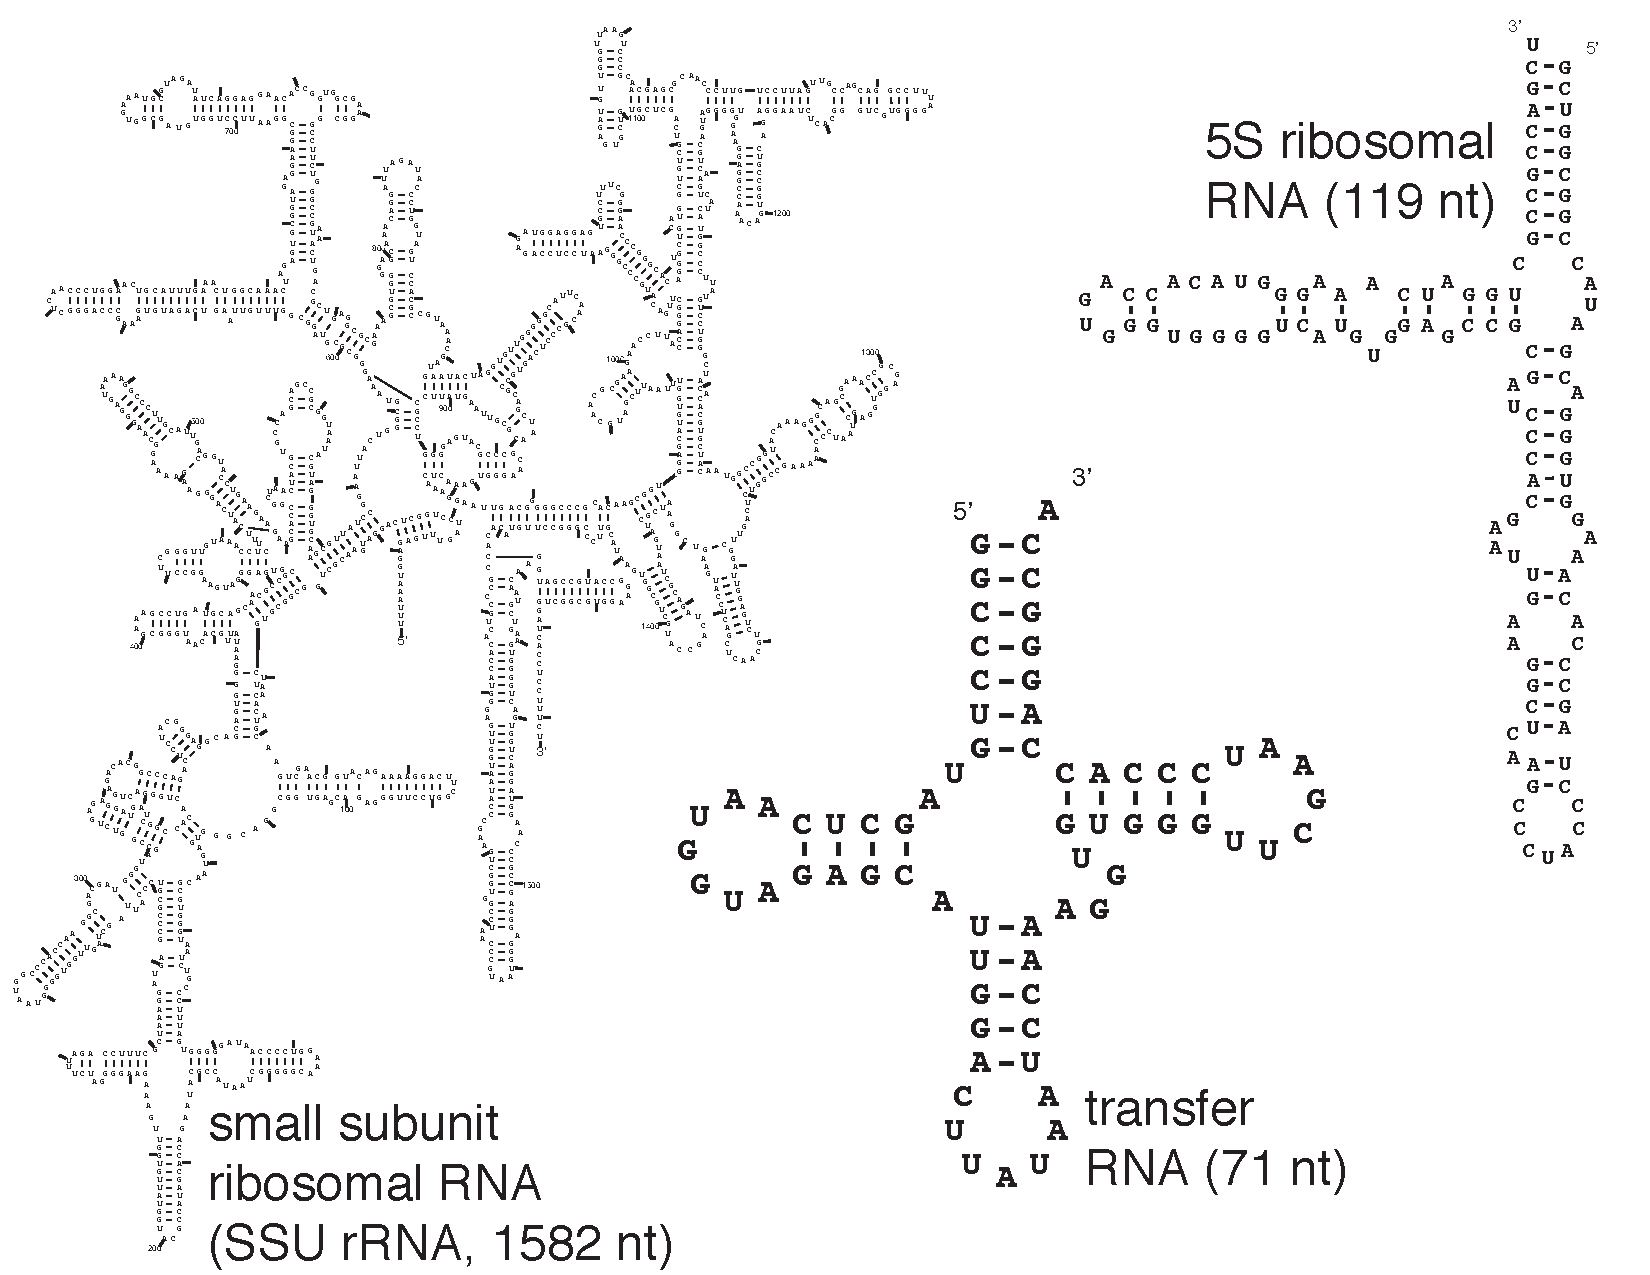
\includegraphics[width=10.5in]{figs/16s-5s-trna-allblack}}
\end{slide}
%%%%%%%%%%%%%%%%%%%%%%%%%%%%%%%%%%%%%%%%%%%%%%%%%%%%%%%%%%%%%%%%%%%%%%
\begin{slide}
\begin{center}
\textbf{Functional RNAs play many vital roles in the cell}
\end{center}
\medskip

\small
\begin{center}
\begin{tabular}{r|l|ccc}
%\item
%  Noncoding RNA (ncRNA): all RNAs other than mRNA
 & key RNAs involved & archaea & bacteria & eukarya \\ \hline
 & \\ 
translation & ribosomal RNAs & x & x & x \\
            & transfer RNAs  & x & x & x \\
            & RNase P RNA    & x & x & x \\
            & snoRNAs        & x &   & x \\ 
            & SRP RNA        & x & x & x \\ 
            & tmRNA          &   & x &   \\ 
            & RNaseMRP       &   &   & x \\ 
            &  \\ 
gene expression & riboswitches & ? & x & ? \\
                & microRNAs &  & & x \\
                & 6S RNA & & & x\\ 
                & \\ 
splicing        & U1, U2, U4, U5, U6 & & & x \\ 
                & \\
other           & telomerase RNA & & & x \\ 
                & Y RNA          & & & x \\
                & Vault RNA      & & & x \\
                & many more... & & & \\ 
\end{tabular}
\end{center}

\vfill
\end{slide}
%%%%%%%%%%%%%%%%%%%%%%%%%%%%%%%%%%%%%%%%%%%%%%%%%%%%%%%%%%%%%%%%%%%%%%
\begin{slide}
\begin{center}
\textbf{Functional RNAs play many vital roles in the cell}
\end{center}
\medskip

\small
\begin{center}
\begin{tabular}{r|l|ccc}
%\item
%  Noncoding RNA (ncRNA): all RNAs other than mRNA
 & key RNAs involved & archaea & bacteria & eukarya \\ \hline
 & \\ 
translation & ribosomal RNAs & x & x & x \\
            & transfer RNAs  & x & x & x \\
            & RNase P RNA    & x & x & x \\
            & snoRNAs        & x &   & x \\ 
            & SRP RNA        & x & x & x \\ 
            & tmRNA          &   & x &   \\ 
            & RNaseMRP       &   &   & x \\ 
            &  \\ 
gene expression & riboswitches & ? & x & ? \\
                & microRNAs &  & & x \\
                & 6S RNA & & & x\\ 
                & \\ 
splicing        & U1, U2, U4, U5, U6 & & & x \\ 
                & \\
other           & telomerase RNA & & & x \\ 
                & Y RNA          & & & x \\
                & Vault RNA      & & & x \\
                & many more... & & & \\ 
\end{tabular}


\center{
\includegraphics[width=2.5in]{figs/rfam-logo}}

database of more than 2400 non-coding RNA families \\ each represented by a
secondary structure, alignment, and covariance model.
\end{center}

\vfill
\end{slide}
%%%%%%%%%%%%%%%%%%%%%%%%%%%%%%%%%%%%%%%%%%%%%%%%%%%%%%%%%%%%%%%%%%%%%%
\begin{slide}
\begin{center}
\textbf{Outline of talk}

\small
\begin{description}
\item[1.] Motivation: collecting homologs facilitates comparative
  sequence analysis.\\ 1965: Secondary structure determination of
  transfer RNA.
\item[2.] Sequence and sequence+structure profiles
%\item[3.] Benchmarking RNA homology search
\item[3.] Accelerating RNA homology search
\item[4.] Implications for Rfam
\item[5.] New features in latest version of Infernal
\end{description}

\end{center}
\vfill
\end{slide}
%%%%%%%%%%%%%%%%%%%%%%%%%%%%%%%%%%%%%%%%%%%%%%%%%%%%%%%%%%%%%%%%%%%%
\begin{slide}
\center{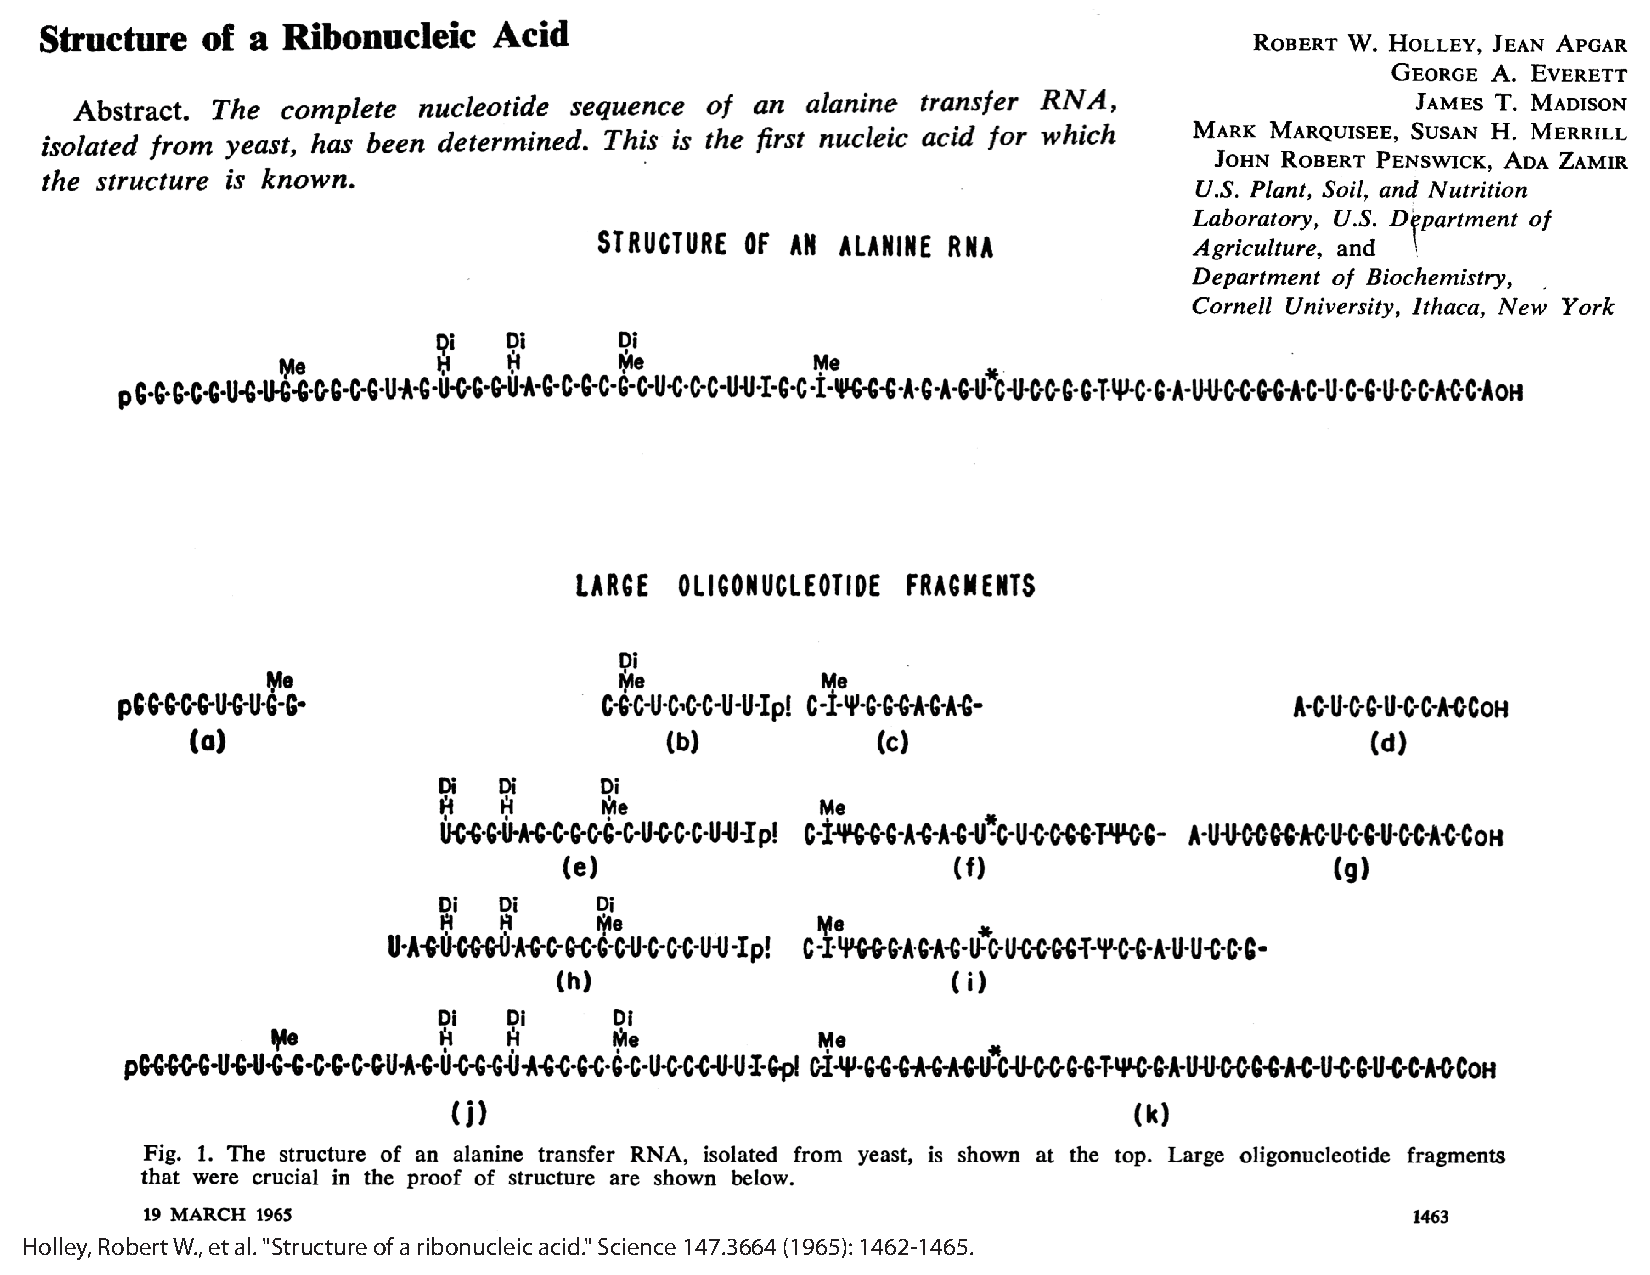
\includegraphics[width=10.5in]{figs/trna-covariation1}}
\end{slide}
%%%%%%%%%%%%%%%%%%%%%%%%%%%%%%%%%%%%%%%%%%%%%%%%%%%%%%%%%%%%%%%%%%%%
\begin{slide}
\center{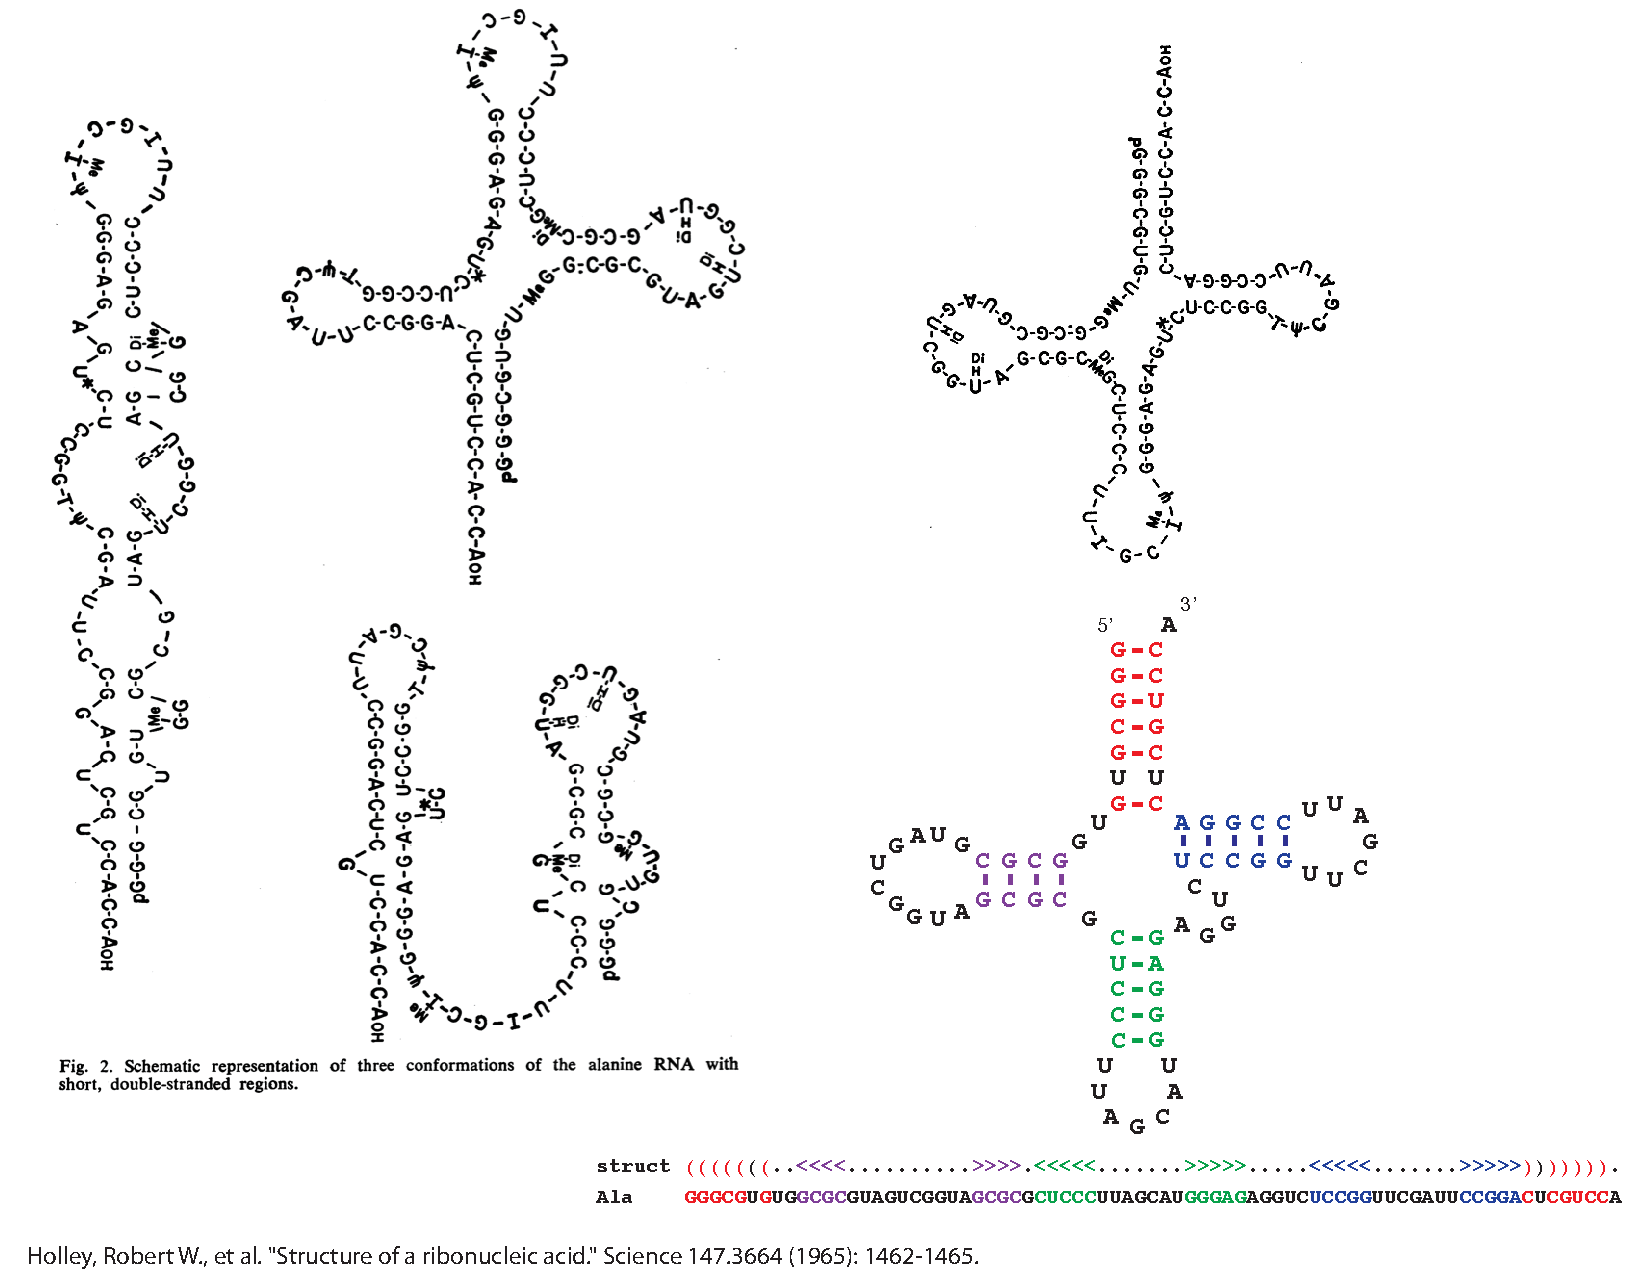
\includegraphics[width=10.5in]{figs/trna-covariation2}}
\end{slide}
%%%%%%%%%%%%%%%%%%%%%%%%%%%%%%%%%%%%%%%%%%%%%%%%%%%%%%%%%%%%%%%%%%%%
%\begin{slide}
%\center{\includegraphics[width=10.5in]{figs/trna-covariation3a}}
%\end{slide}
%%%%%%%%%%%%%%%%%%%%%%%%%%%%%%%%%%%%%%%%%%%%%%%%%%%%%%%%%%%%%%%%%%%%
\begin{slide}
\center{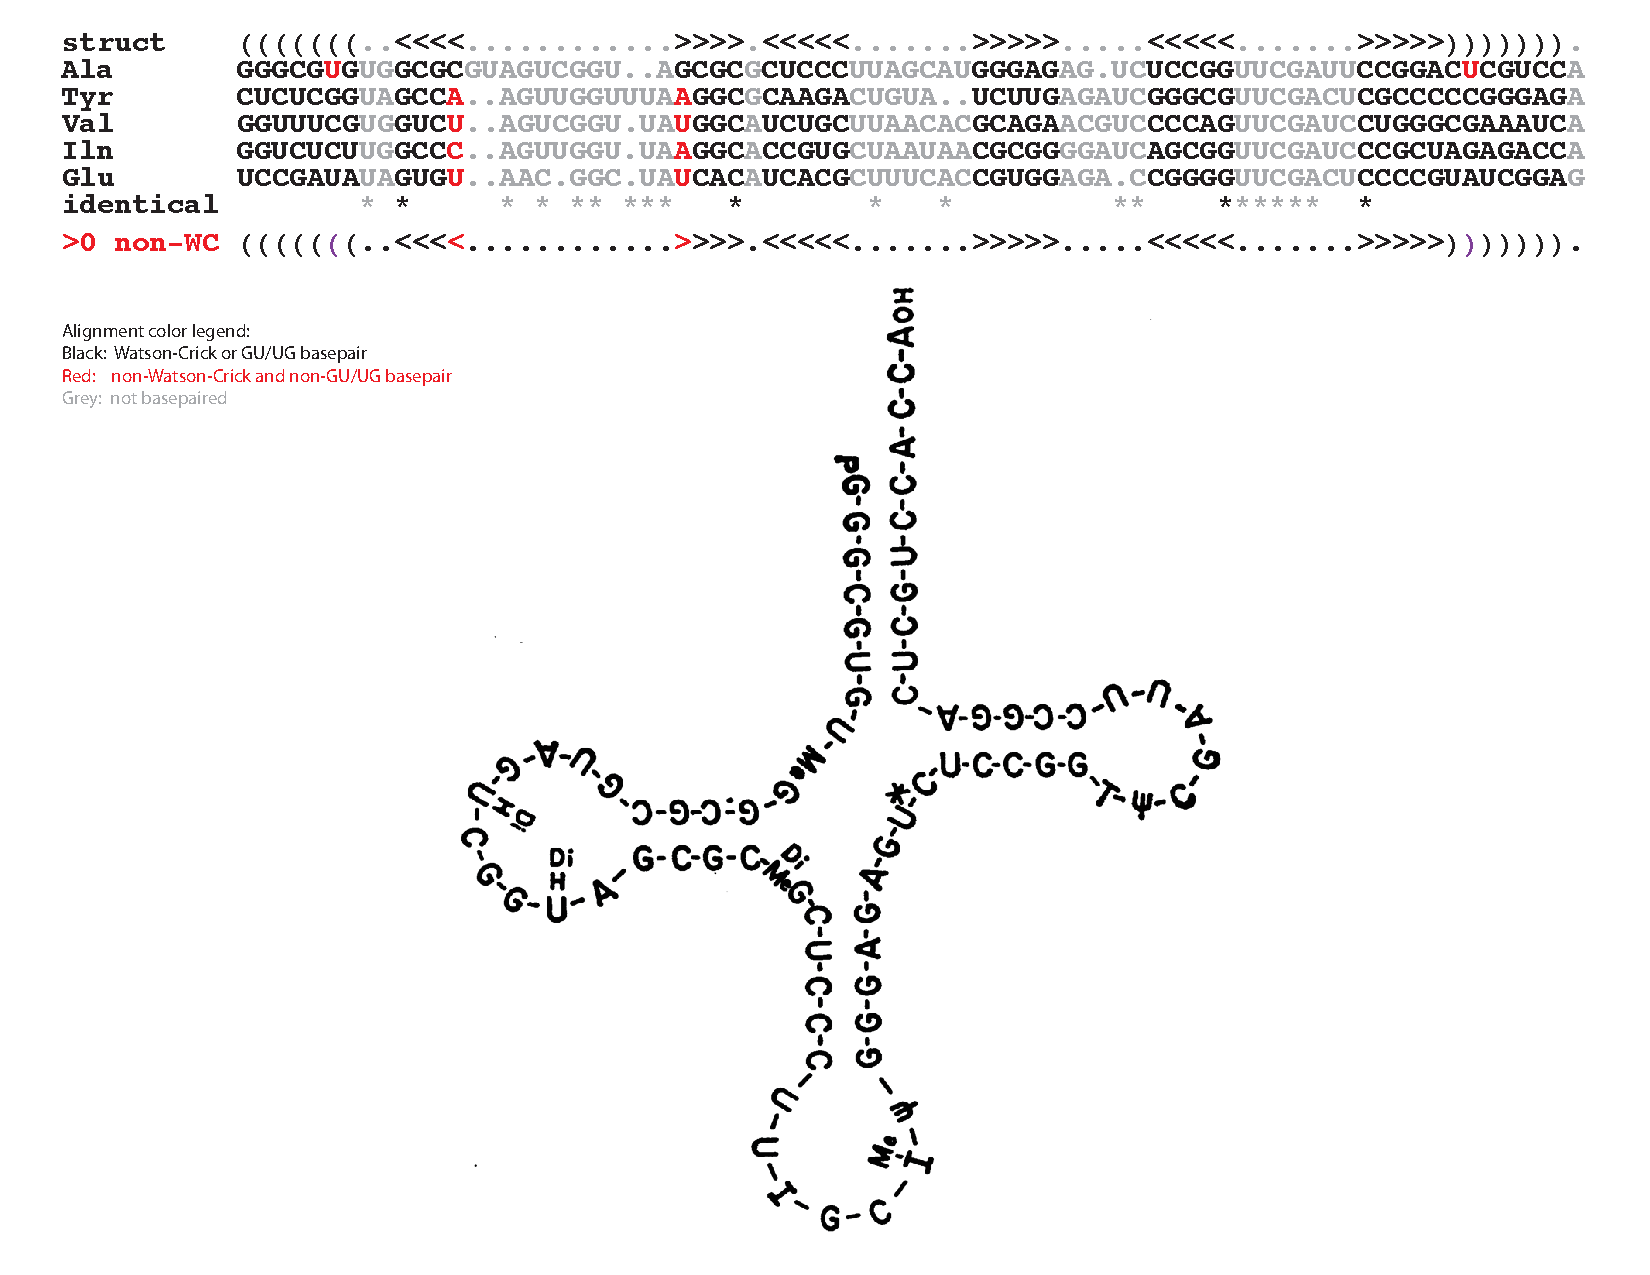
\includegraphics[width=10.5in]{figs/trna-covariation3b}}
\end{slide}
%%%%%%%%%%%%%%%%%%%%%%%%%%%%%%%%%%%%%%%%%%%%%%%%%%%%%%%%%%%%%%%%%%%%
%\begin{slide}
%\center{\includegraphics[width=10.5in]{figs/trna-covariation4a}}
%\end{slide}
%%%%%%%%%%%%%%%%%%%%%%%%%%%%%%%%%%%%%%%%%%%%%%%%%%%%%%%%%%%%%%%%%%%%
\begin{slide}
\center{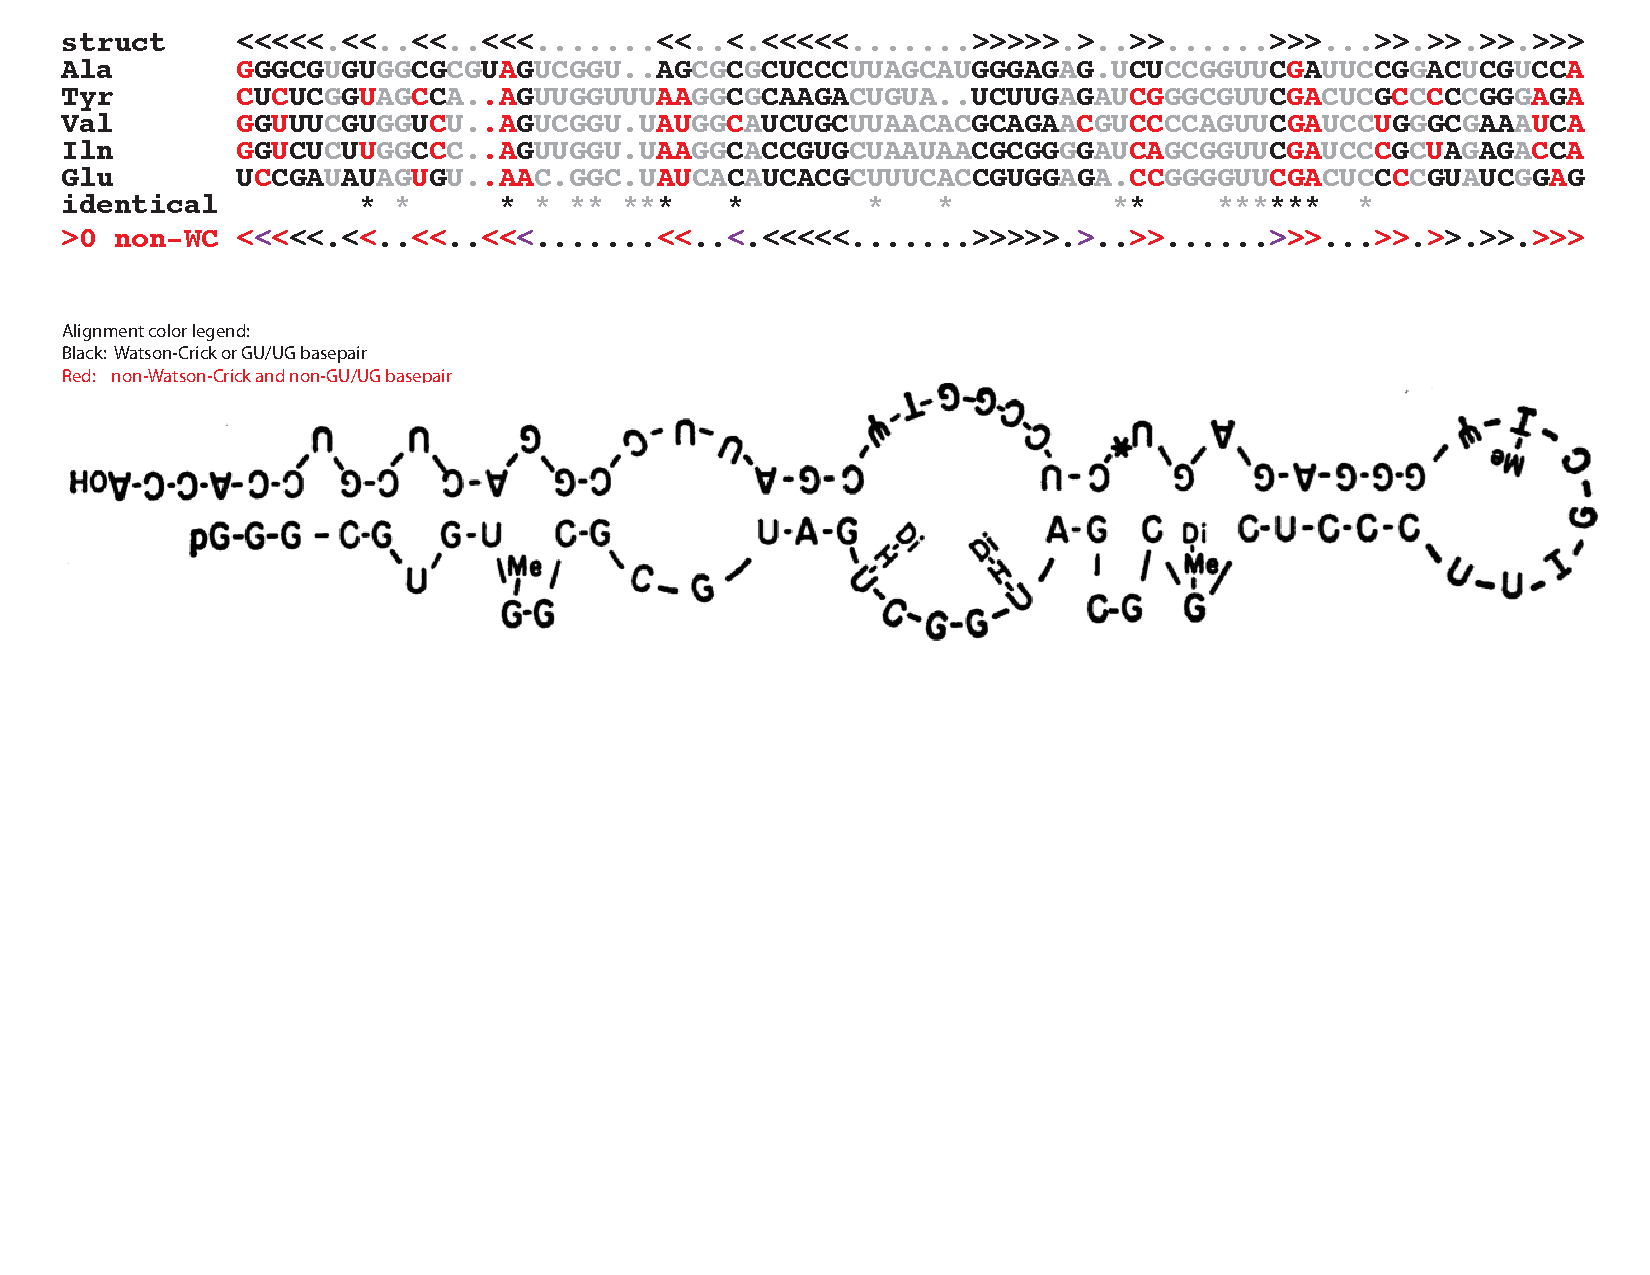
\includegraphics[width=10.5in]{figs/trna-covariation4b}}
\end{slide}
%%%%%%%%%%%%%%%%%%%%%%%%%%%%%%%%%%%%%%%%%%%%%%%%%%%%%%%%%%%%%%%%%%%%
\begin{slide}
\center{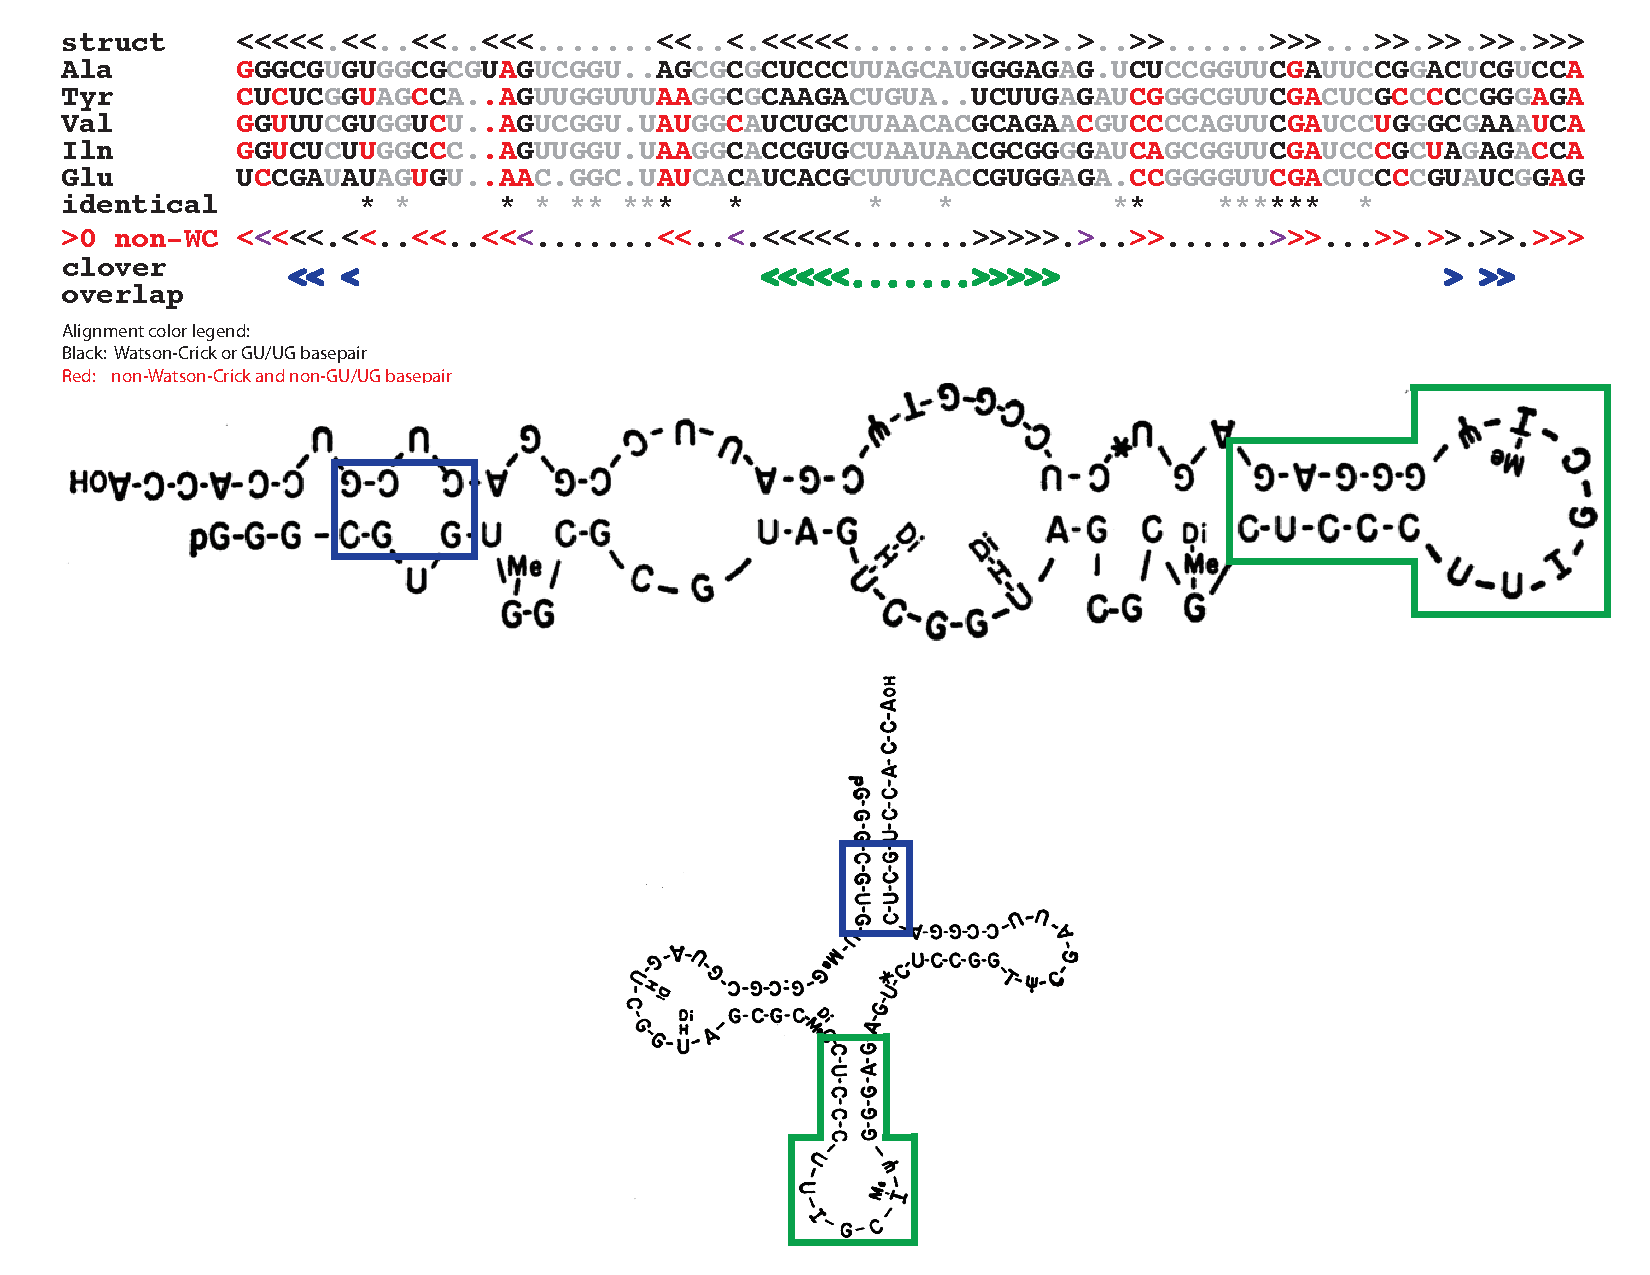
\includegraphics[width=10.5in]{figs/trna-covariation4c}}
\end{slide}
%%%%%%%%%%%%%%%%%%%%%%%%%%%%%%%%%%%%%%%%%%%%%%%%%%%%%%%%%%%%%%%%%%%%
%\begin{slide}
%\center{\includegraphics[width=10.5in]{figs/trna-covariation5a}}
%\end{slide}
%%%%%%%%%%%%%%%%%%%%%%%%%%%%%%%%%%%%%%%%%%%%%%%%%%%%%%%%%%%%%%%%%%%%
\begin{slide}
\center{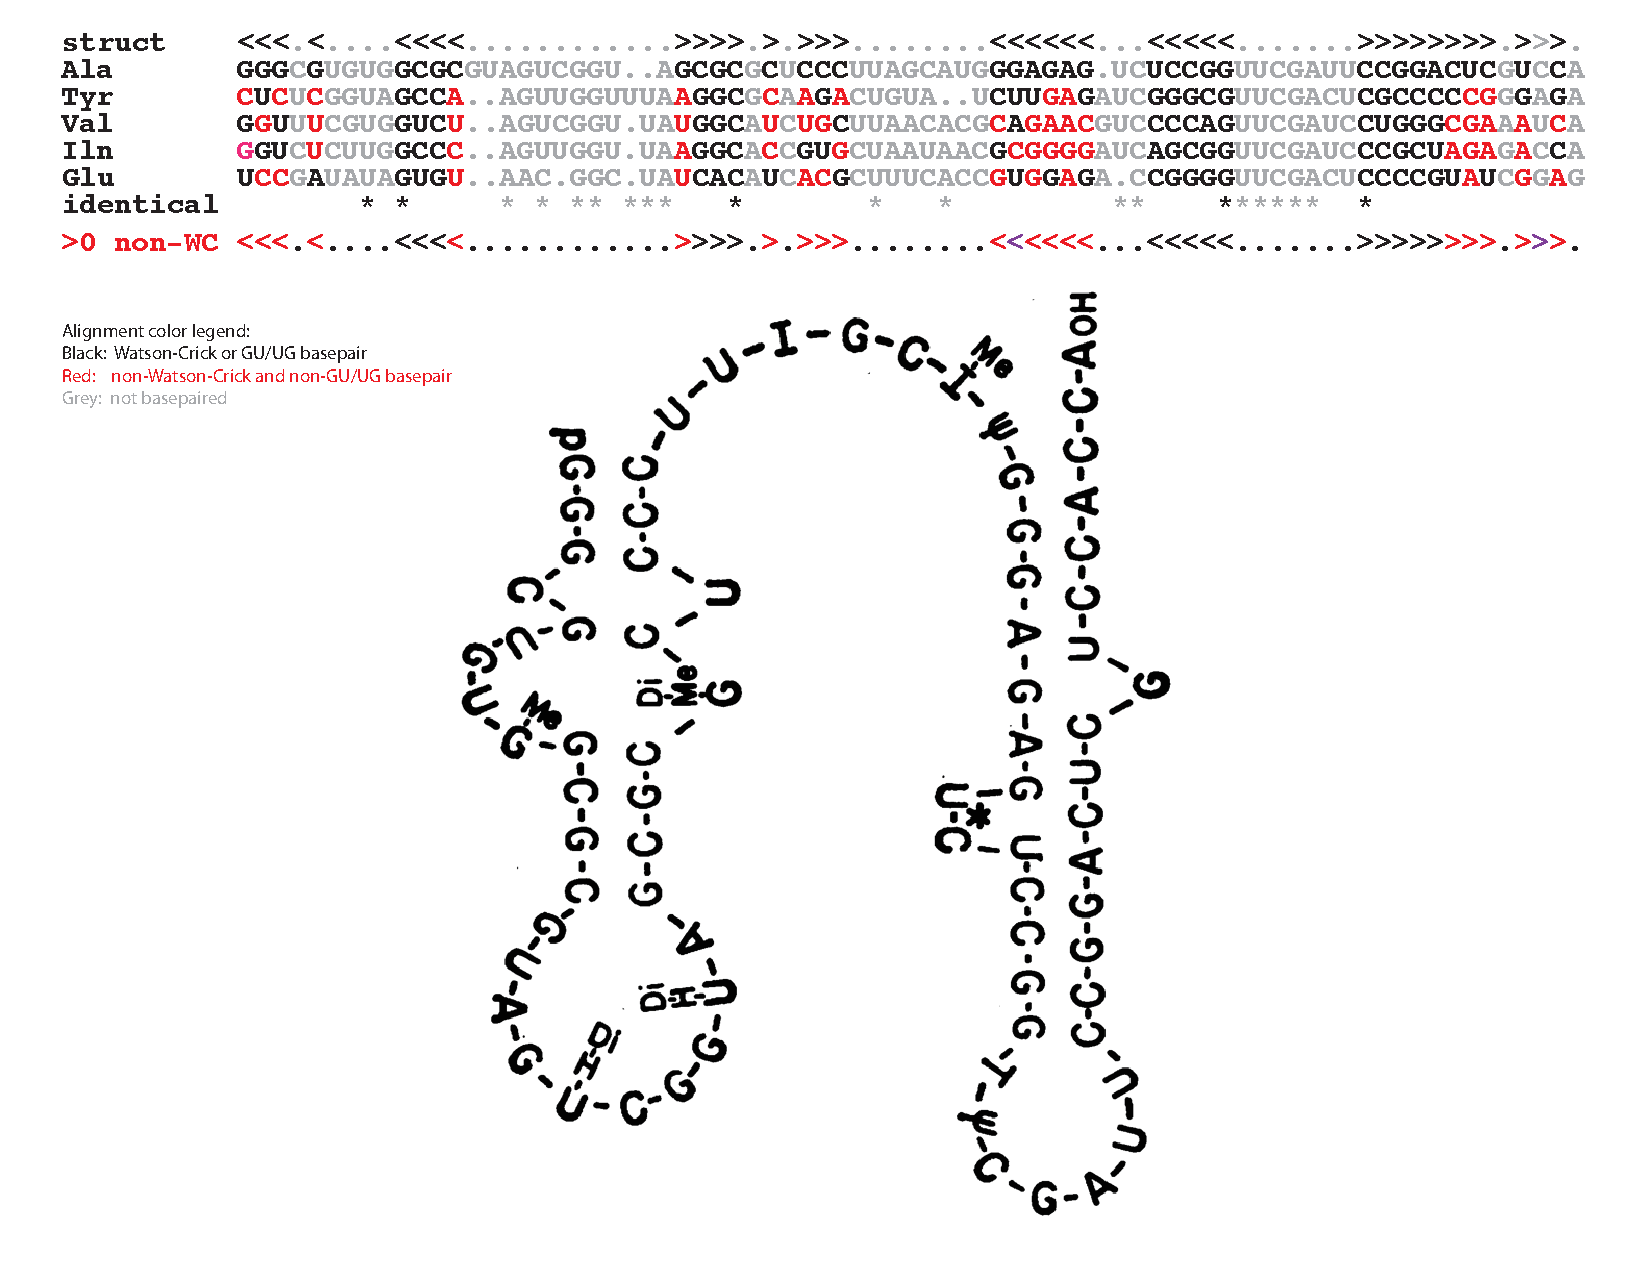
\includegraphics[width=10.5in]{figs/trna-covariation5b}}
\end{slide}
%%%%%%%%%%%%%%%%%%%%%%%%%%%%%%%%%%%%%%%%%%%%%%%%%%%%%%%%%%%%%%%%%%%%
\begin{slide}
\center{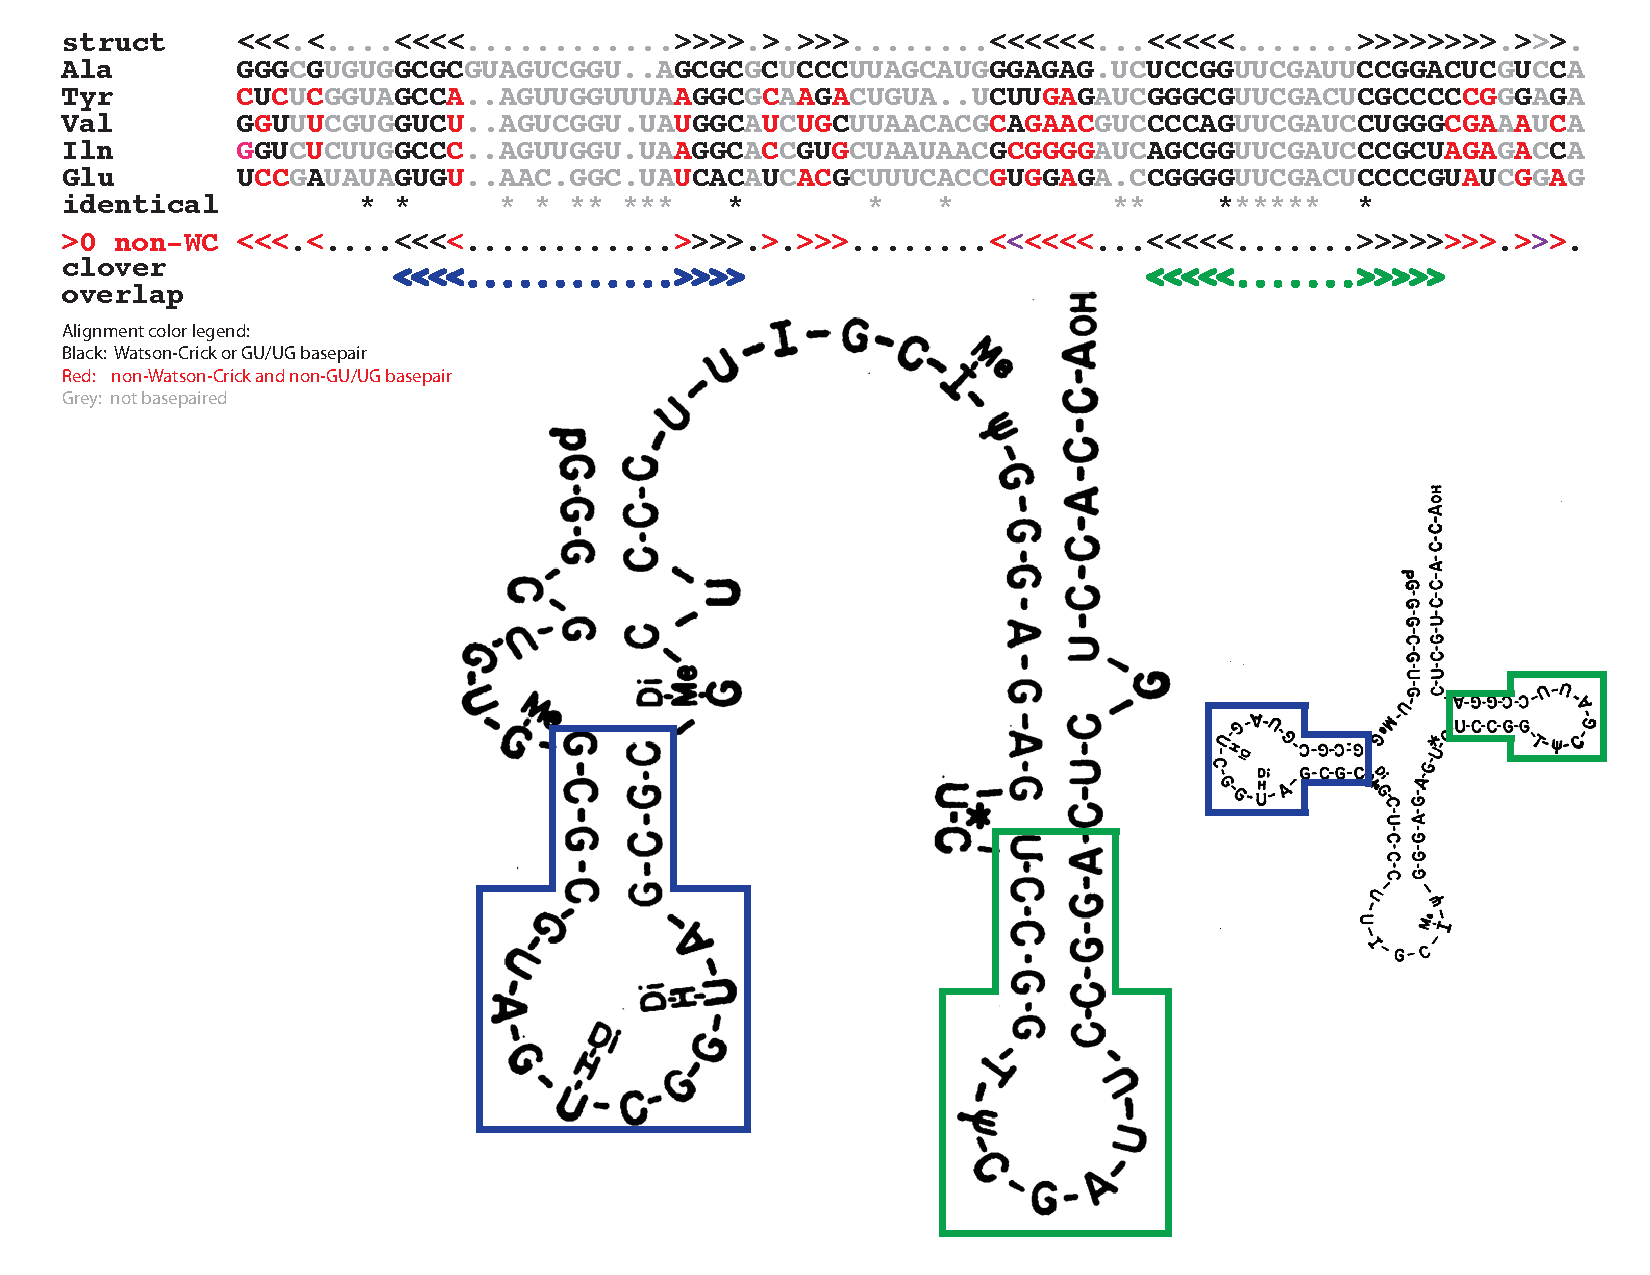
\includegraphics[width=10.5in]{figs/trna-covariation5c}}
\end{slide}
%%%%%%%%%%%%%%%%%%%%%%%%%%%%%%%%%%%%%%%%%%%%%%%%%%%%%%%%%%%%%%%%%%%%
\begin{slide}
\center{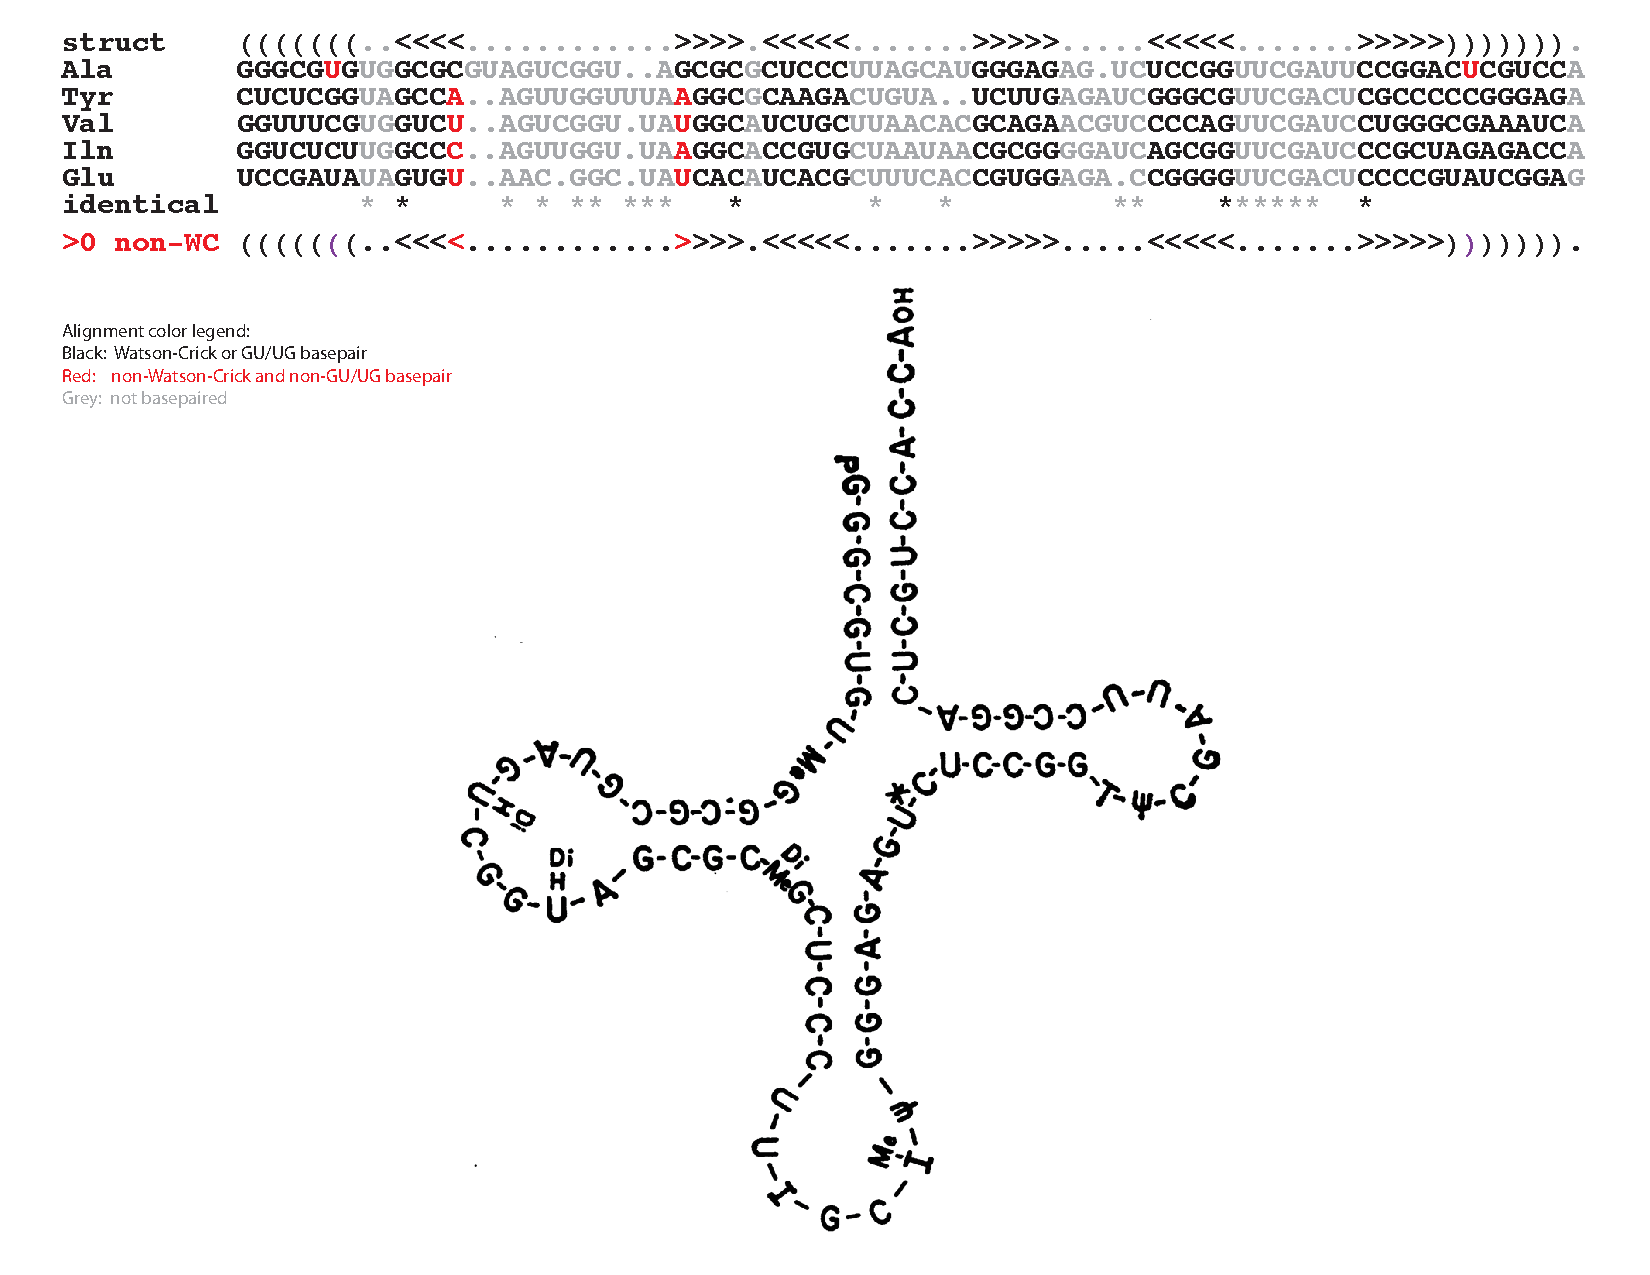
\includegraphics[width=10.5in]{figs/trna-covariation3b}}
\end{slide}
%%%%%%%%%%%%%%%%%%%%%%%%%%%%%%%%%%%%%%%%%%%%%%%%%%%%%%%%%%%%%%%%%%%%
\begin{slide}
\center{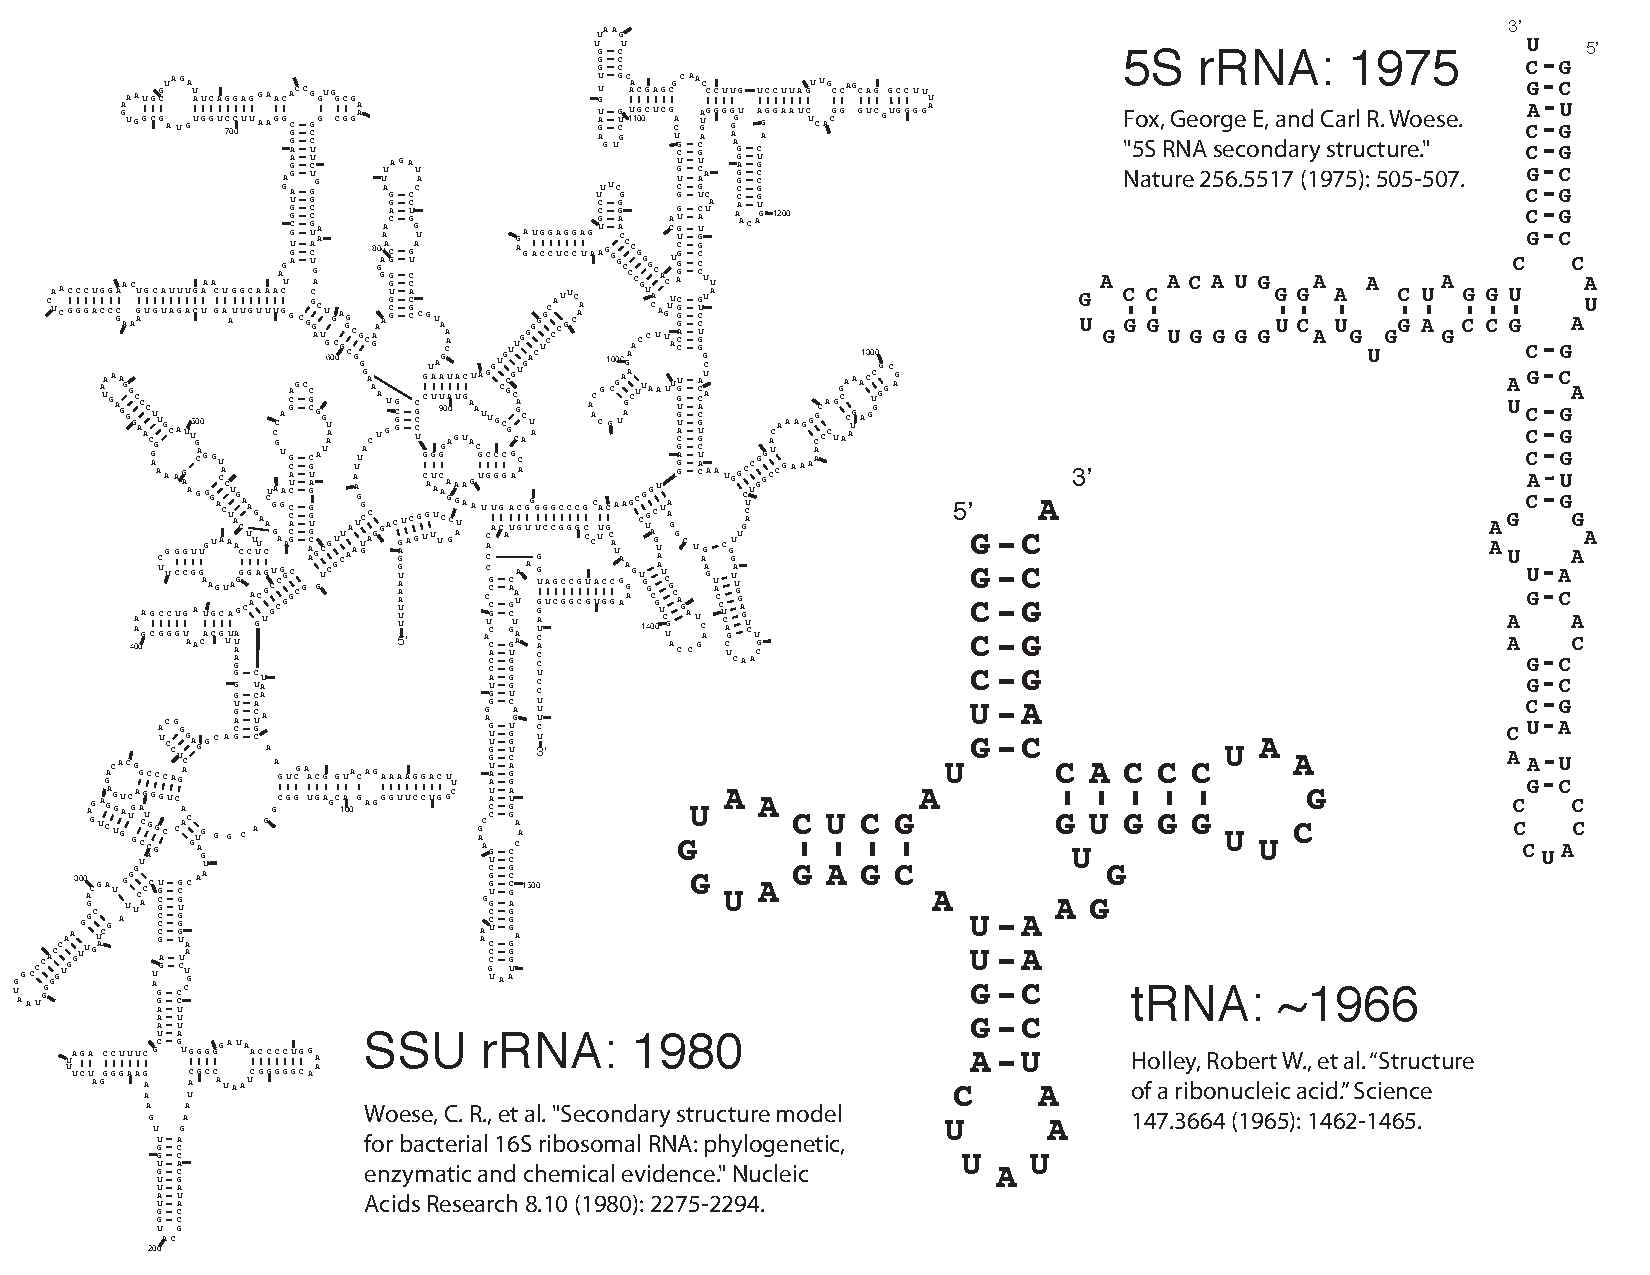
\includegraphics[width=10.5in]{figs/16s-5s-trna-allblack-dates-refs}}
\end{slide}
%%%%%%%%%%%%%%%%%%%%%%%%%%%%%%%%%%%%%%%%%%%%%%%%%%%%%%%%%%%%%%%%%%%%
%\begin{slide}
%\center{\includegraphics[width=10.5in]{figs/16s-5s-trna-bpcolored}}
%\end{slide}
%%%%%%%%%%%%%%%%%%%%%%%%%%%%%%%%%%%%%%%%%%%%%%%%%%%%%%%%%%%%%%%%%%%%
%%%%%%%%%%%%%%%%%%%%%%%%%%%%%%%%%%%%%%%%%%%%%%%%%%%%%%%%%%%%%%%%%%%%
% RAN OUT OF TIME, COULDN'T MAKE THIS SLIDE:
\begin{comment}
\begin{slide}

\center{\textbf{TODO: Slide showing which conserved parts of 16S do what}}

\vfill
\end{slide}
\end{comment}
%%%%%%%%%%%%%%%%%%%%%%%%%%%%%%%%%%%%%%%%%%%%%%%%%%%%%%%%%%%%%%%%%%%%
\begin{slide}

\center{\textbf{Comparative sequence analysis \\
    of homologs informs biologists}}

%\small
\begin{itemize}
\item Inference of  structure
%  \begin{itemize}
%  \item tRNA (Holley, 1965)
%  \item SSU rRNA (Woese, 1980)
%  \end{itemize}
\item Inference of phylogeny of organisms
%\item Inference of which biological processes are being carried out
\item Inference of functional regions based on conservation levels
\end{itemize}

\vfill
\end{slide}
%%%%%%%%%%%%%%%%%%%%%%%%%%%%%%%%%%%%%%%%%%%%%%%%%%%%%%%%%%%%%%%%%%%%%%
\begin{slide}
\center{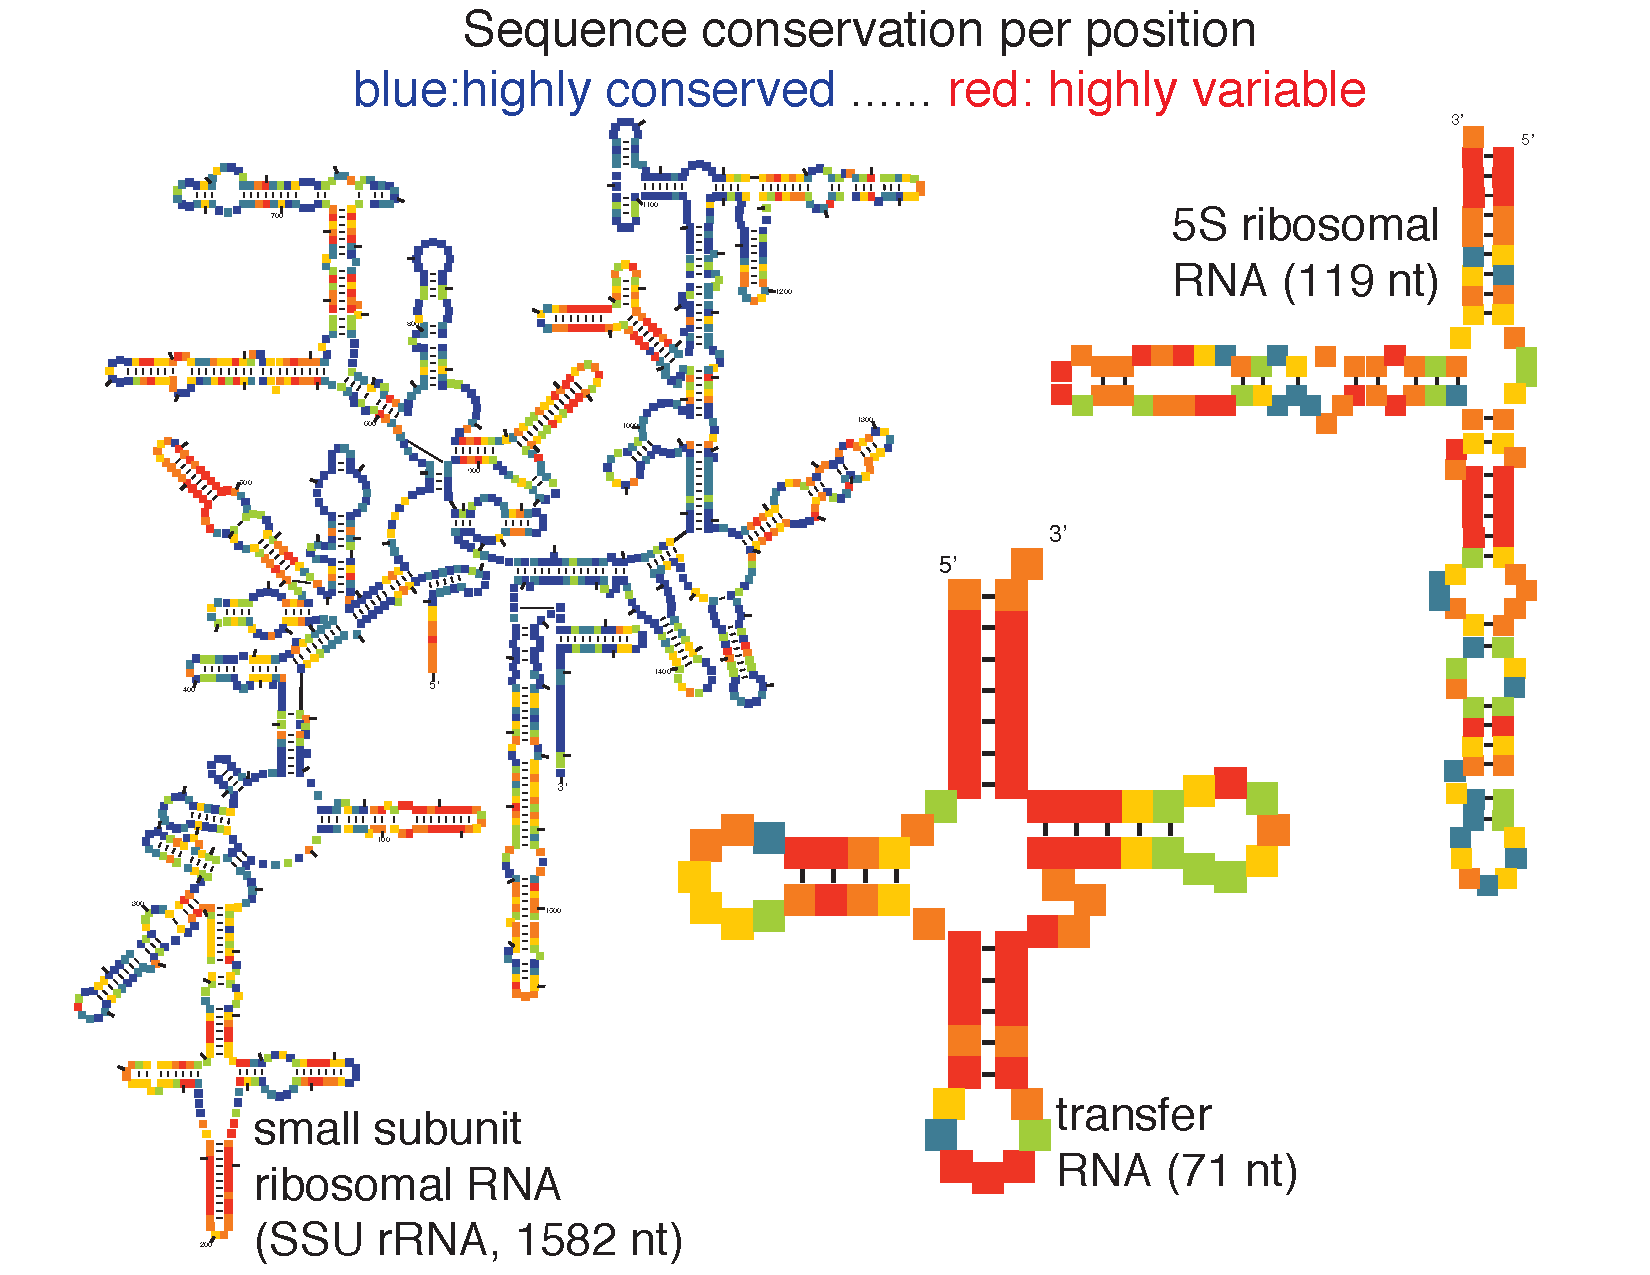
\includegraphics[width=10.5in]{figs/16s-5s-trna-info}}
\end{slide}
%%%%%%%%%%%%%%%%%%%%%%%%%%%%%%%%%%%%%%%%%%%%%%%%%%%%%%%%%%%%%%%%%%%%
\begin{slide}

\center{\textbf{Comparative sequence analysis \\
    of homologs informs biologists}}

%\small
\begin{itemize}
\item Inference of  structure
%  \begin{itemize}
%  \item tRNA (Holley, 1965)
%  \item SSU rRNA (Woese, 1980)
%  \end{itemize}
\item Inference of phylogeny of organisms
%\item Inference of which biological processes are being carried out
\item Inference of functional regions based on conservation levels
\end{itemize}

\medskip
\medskip
\normalsize
\begin{center}
\textbf{Computational homology search methods use \\ one or more known
family members to find additional homologs.}
\end{center}

\vfill
\end{slide}
%%%%%%%%%%%%%%%%%%%%%%%%%%%%%%%%%%%%%%%%%%%%%%%%%%%%%%%%%%%%%%%%%%%%
\begin{slide}
\begin{center}
\textbf{Outline of talk}

\begin{description}
\item[1.] Motivation: collecting homologs facilitates comparative
  sequence analysis.\\ 1965: Secondary structure determination of
  transfer RNA.
\item[\textcolor{red}{2.}] \textcolor{red}{Sequence and sequence+structure profiles}
%\item[3.] Benchmarking RNA homology search
\item[3.] Accelerating RNA homology search
\item[4.] Implications for Rfam
\item[5.] New features in latest version of Infernal
\end{description}

\end{center}
\vfill
\end{slide}
%%%%%%%%%%%%%%%%%%%%%%%%%%%%%%%%%%%%%%%%%%%%%%%%%%%%%%%%%%%%%%%%%%%%
\begin{slide}
\begin{center}
%\textbf{Comparative analysis of sequence families}: \\
\textbf{Sequence conservation provides \\ information for homology searches}

\medskip
Conservation levels vary across alignment columns.

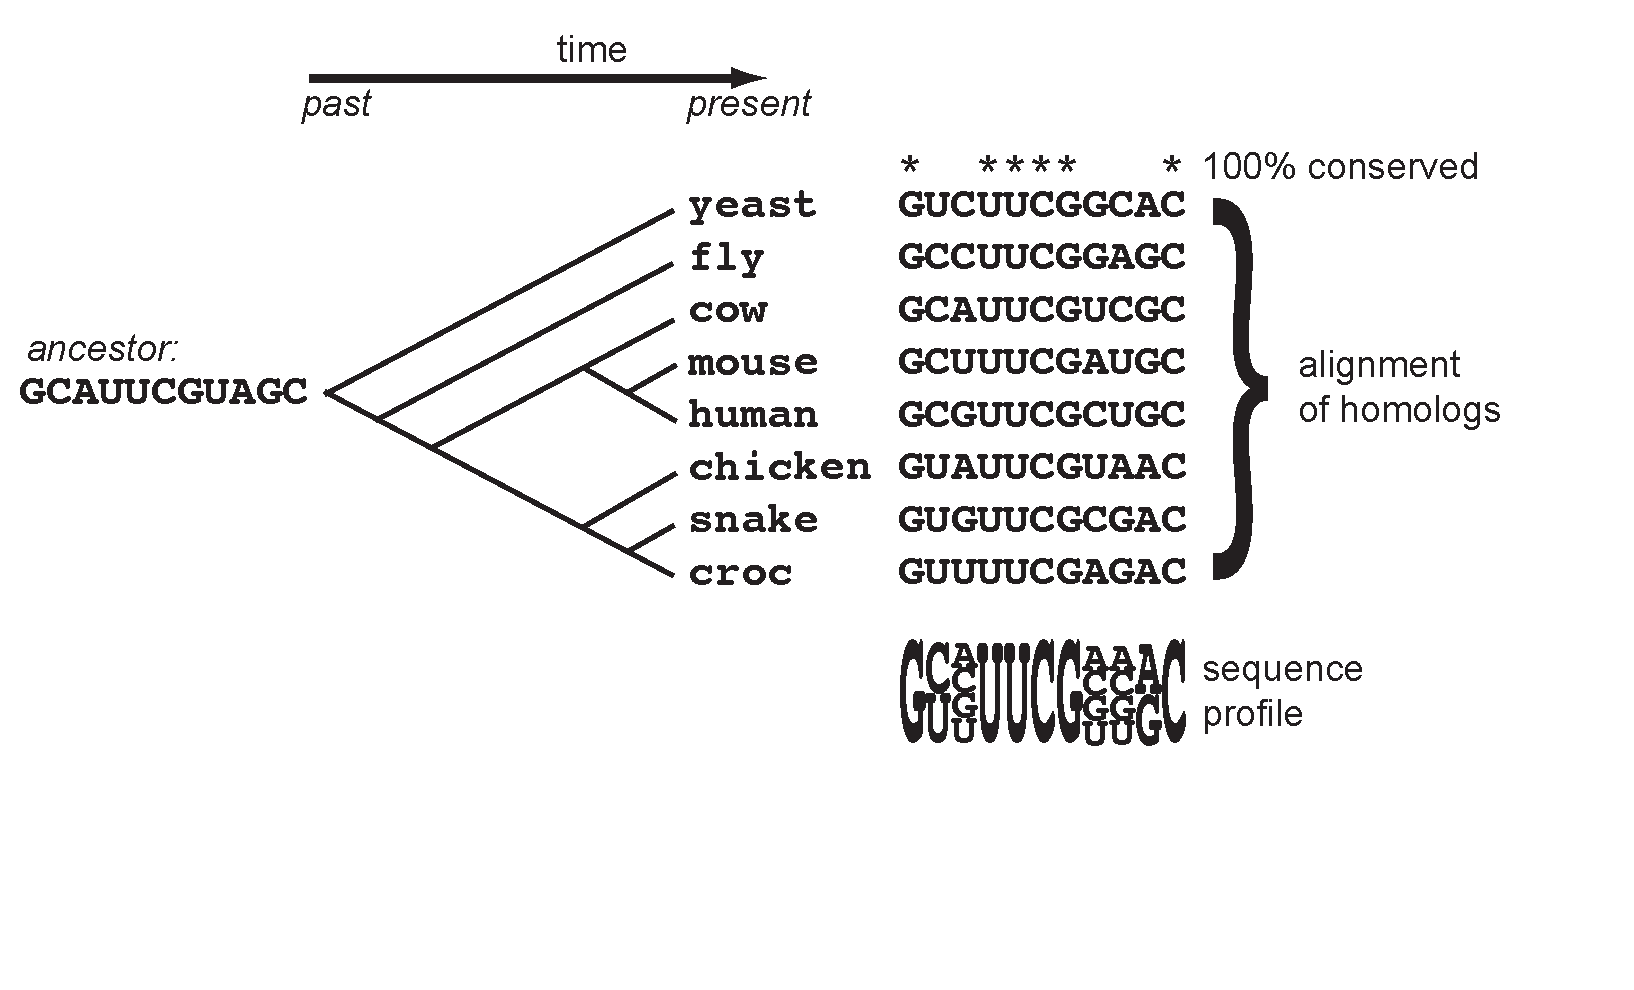
\includegraphics[width=10in]{figs/seqstructprofiles-seq1}
\end{center}

\vfill
\end{slide}
%%%%%%%%%%%%%%%%%%%%%%%%%%%%%%%%%%%%%%%%%%%%%%%%%%%%%%%%%%%%%%%%%%%%%%
\begin{slide}
\begin{center}
\textbf{Structure conservation provides additional information}
\medskip

Base-paired positions covary \\ to maintain Watson-Crick complementarity.

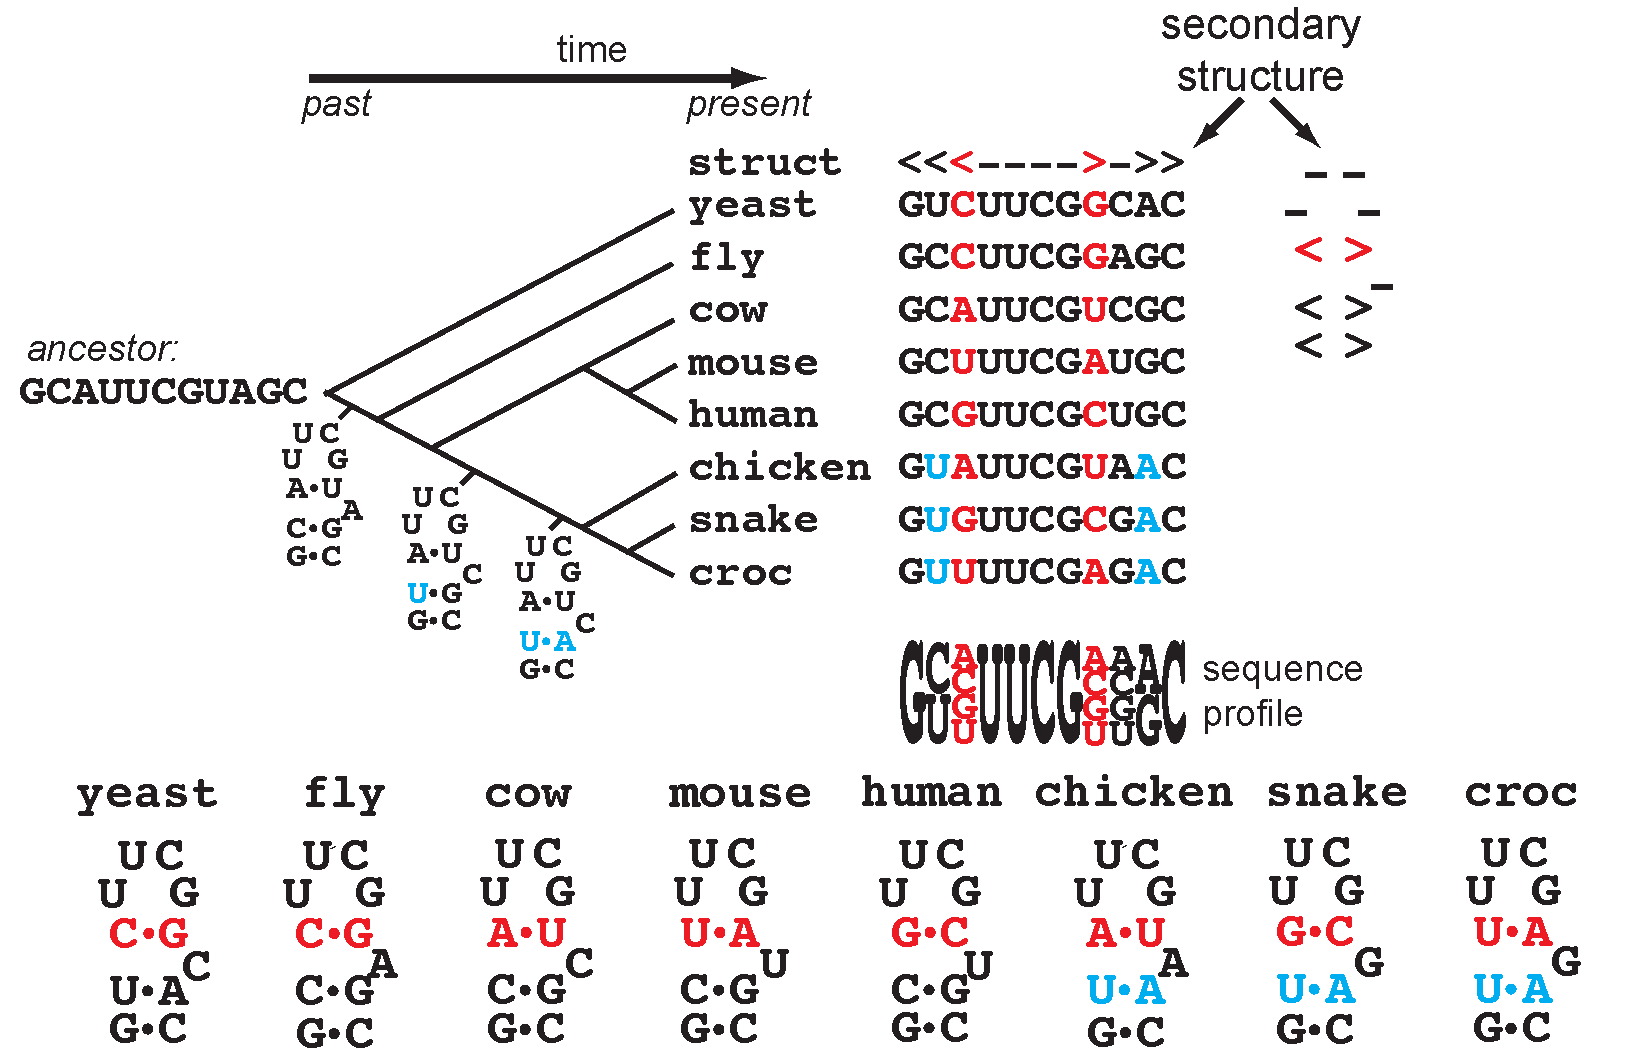
\includegraphics[width=10in]{figs/seqstructprofiles-struct2}
\end{center}

\vfill
\end{slide}
%%%%%%%%%%%%%%%%%%%%%%%%%%%%%%%%%%%%%%%%%%%%%%%%%%%%%%%%%%%%%%%%%%%%%%%%%%
\begin{slide}
\begin{center}
\textbf{Amount of information in a profile can be measured in bits}
\medskip

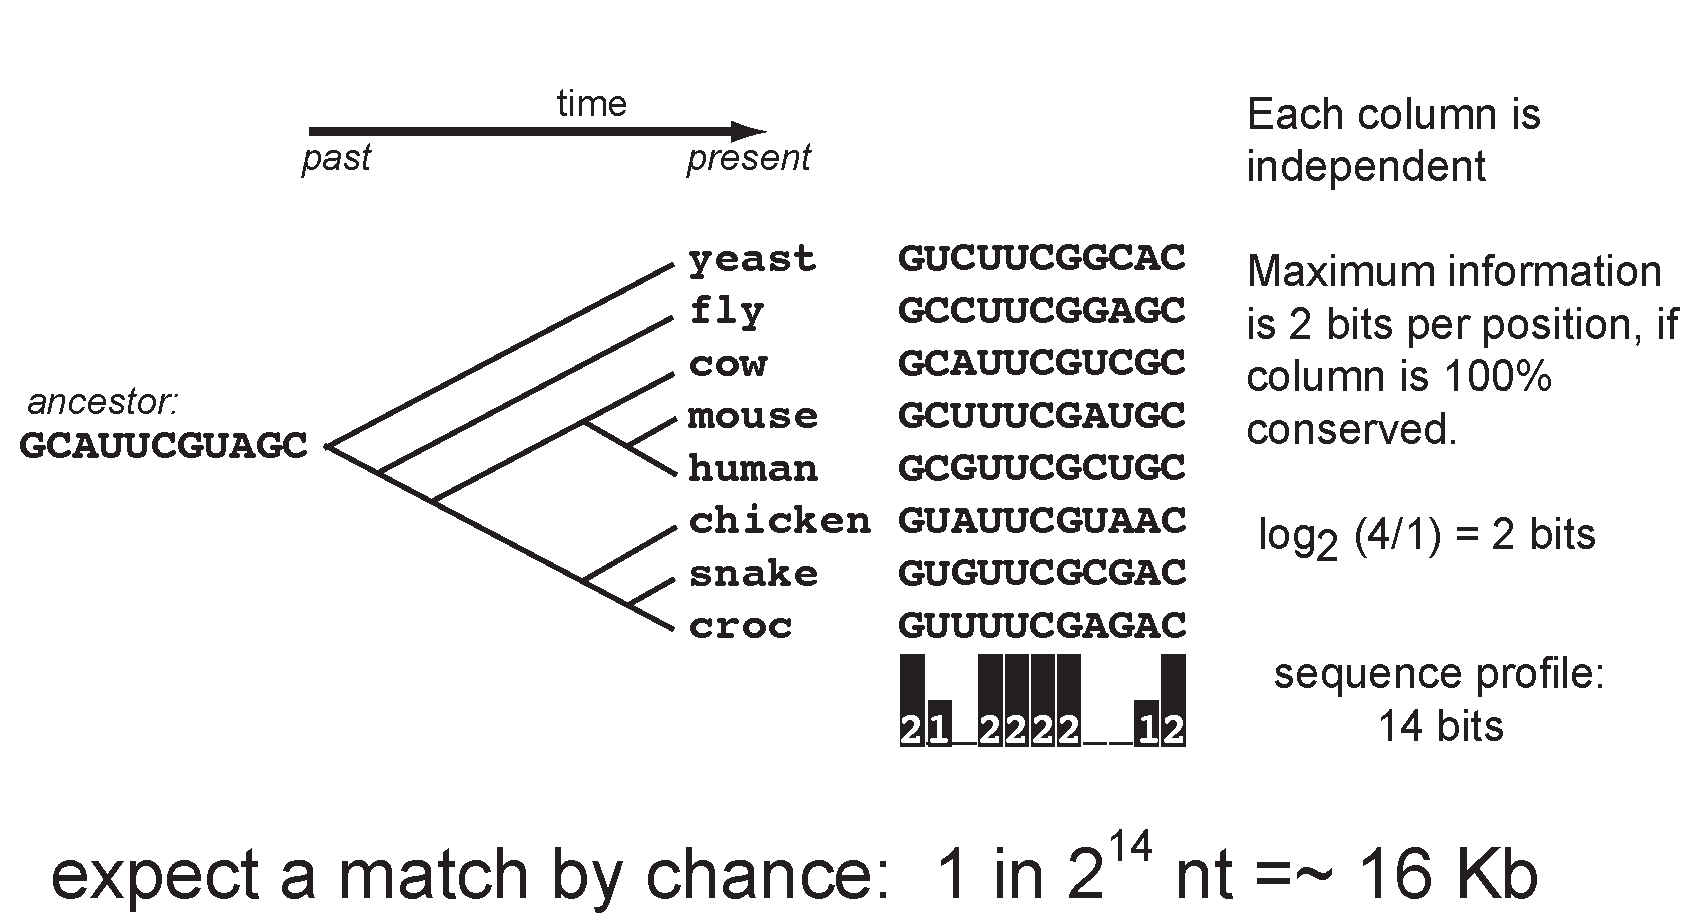
\includegraphics[width=9in]{figs/seqstructprofiles-2014-seqinfo}
\end{center}

\vfill
\end{slide}
%%%%%%%%%%%%%%%%%%%%%%%%%%%%%%%%%%%%%%%%%%%%%%%%%%%%%%%%%%%%%%%%%%%%%%%%%%
\begin{slide}
\begin{center}
\textbf{Structure contributes additional information from covariation}
\medskip

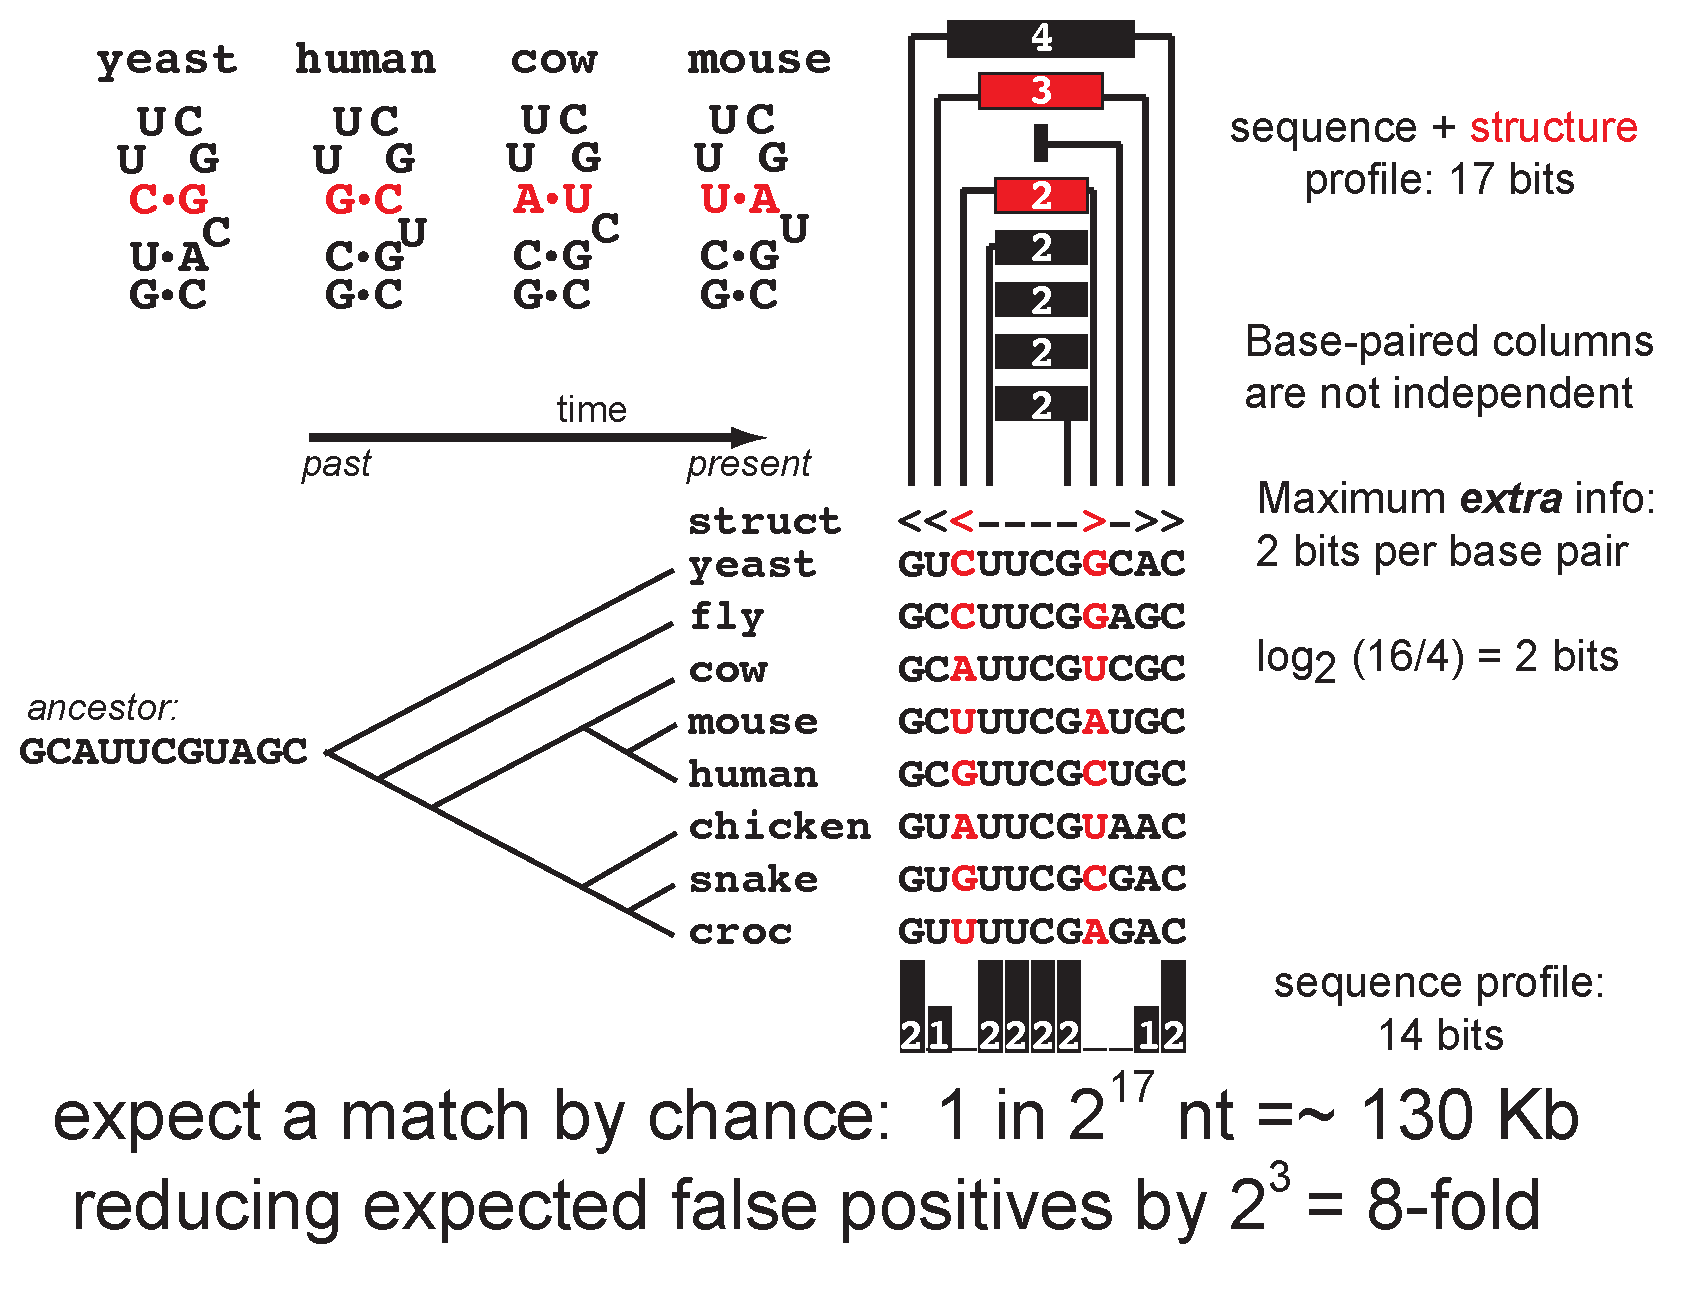
\includegraphics[width=9in]{figs/seqstructprofiles-2014-structinfo}
\end{center}

\vfill
\end{slide}
%%%%%%%%%%%%%%%%%%%%%%%%%%%%%%%%%%%%%%%%%%%%%%%%%%%%%%%%%%%%%%%%%%%%%%%%%%
\begin{slide}
\begin{center}
\textbf{Levels of sequence and structure conservation in RNA families}
\end{center}
\medskip

\begin{center}
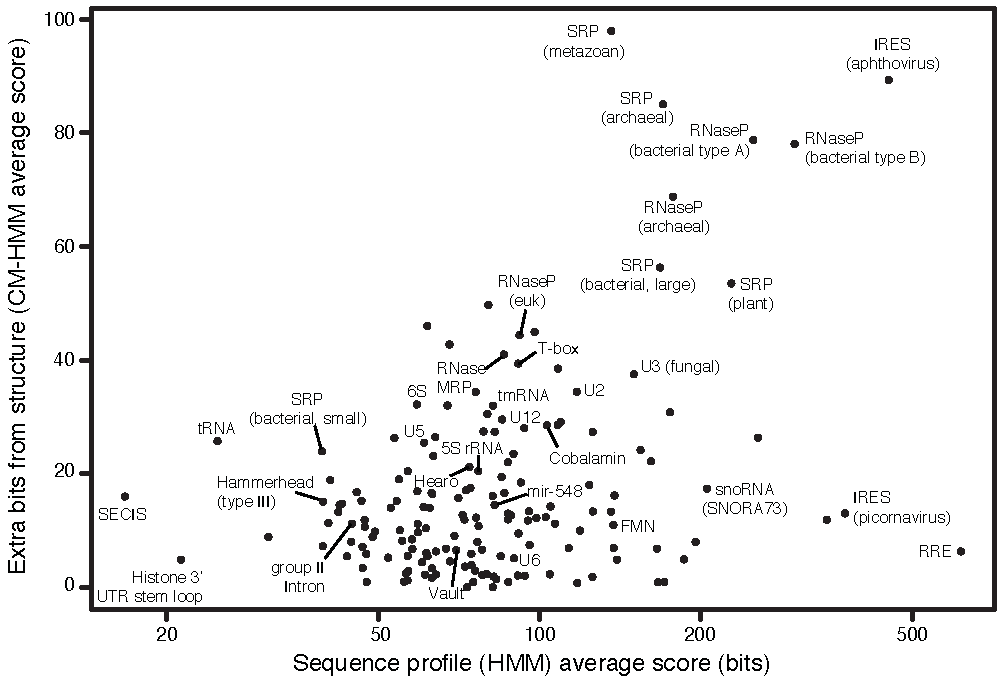
\includegraphics[height=6.5in]{figs/avgscores-rfam11}
\end{center}

\vfill

\end{slide}
%%%%%%%%%%%%%%%%%%%%%%%%%%%%%%%%%%%%%%%%%%%%%%%%%%%%%%%%%%%%%%%%%%%
\begin{slide}
\begin{center}
%\textbf{profile HMMs and covariance models}
\textbf{Eddy lab software for profile probabilistic models } (since 1994)
\end{center}
\medskip

\begin{center}
\small
\begin{tabular}{r|cc} 
%             &         & sequence \\
%             & sequence& and structure \\
%             & profiles& profiles \\ \hline
             & sequence & sequence and \\
             & profiles & structure profiles \\ \hline
  \\
  models     & profile HMMs     & {\color{red} covariance models (CMs)} \\ 
  \\
  software   & {\sc HMMER}      & {\sc Infernal} \\ 
  \\
  main use   & proteins,         & structural RNAs \\ 
             & repetitive DNA elements &  \\
  \\
  databases  & {\sc Pfam} and \sc{Dfam}       & {\sc Rfam} \\
             & (16306 and 4150 entries) & (2474 families) \\
  \\
%  primary sequence & yes & yes \\
%  \\
%  secondary structure & no & yes \\
%  \\
%  algorithms & Viterbi, Forward & CYK, Inside \\
%%             & Forward & Inside \\
%             &         & \\
%  complexity & $O(LN)$ & $O(LN^{2} log N)$ \\
%  \\
  performance& faster but    & slower but    \\
  for RNAs   & less accurate & more accurate \\
\end{tabular}

%\hspace{1.2in}\includegraphics[height=2in]{figs/hmmer_logo}\hspace{1.05in}\includegraphics[height=2.6in]{figs/infernal_logo}
\hspace{2.2in}
\includegraphics[height=3.5in]{figs/hmmer-infernal-refs-2015}

\end{center}

\vfill

\end{slide}
%%%%%%%%%%%%%%%%%%%%%%%%%%%%%%%%%%%%%%%%%%%%%%%%%%%%%%%%%%%%%%%
%%%%%%%%%%%%%%%%%%%%%%%%%%%%%%%%%%%%%%%%%%%%%%%%%%%%%%%%%%%%%%%%%%%%%%
%%%%%%%%%%%%%%%%%%%%%%%%%%%%%%%%%%%%%%%%%%%%%%%%%%%%%%%%%%%%%%%
%%%%%%%%%%%%%%%%%%%%%%%%%%%%%%%%%%%%%%%%%%%%%%%%%%%%%%%%%%%%%%%
%%%%%%%%%%%%%%%%%%%%%%%%%%%%%%%%%%%%%%%%%%%%%%%%%%%%%%%%%%%%%%%
%%%%%%%%%%%%%%%%%%%%%%%%%%%%%%%%%%%%%%%%%%%%%%%%%%%%%%%%%%%%%%%
%%%%%%%%%%%%%%%%%%%%%%%%%%%%%%%%%%%%%%%%%%%%%%%%%%%%%%%%%%%%%%%
%%%%%%%%%%%%%%%%%%%%%%%%%%%%%%%%%%%%%%%%%%%%%%%%%%%%%%%%%%%%%%%%%%%%
\begin{slide}
\begin{center}
%\textbf{profile HMMs and covariance models}
\textbf{Profile HMMs: sequence family models built from alignments}
\end{center}

\center{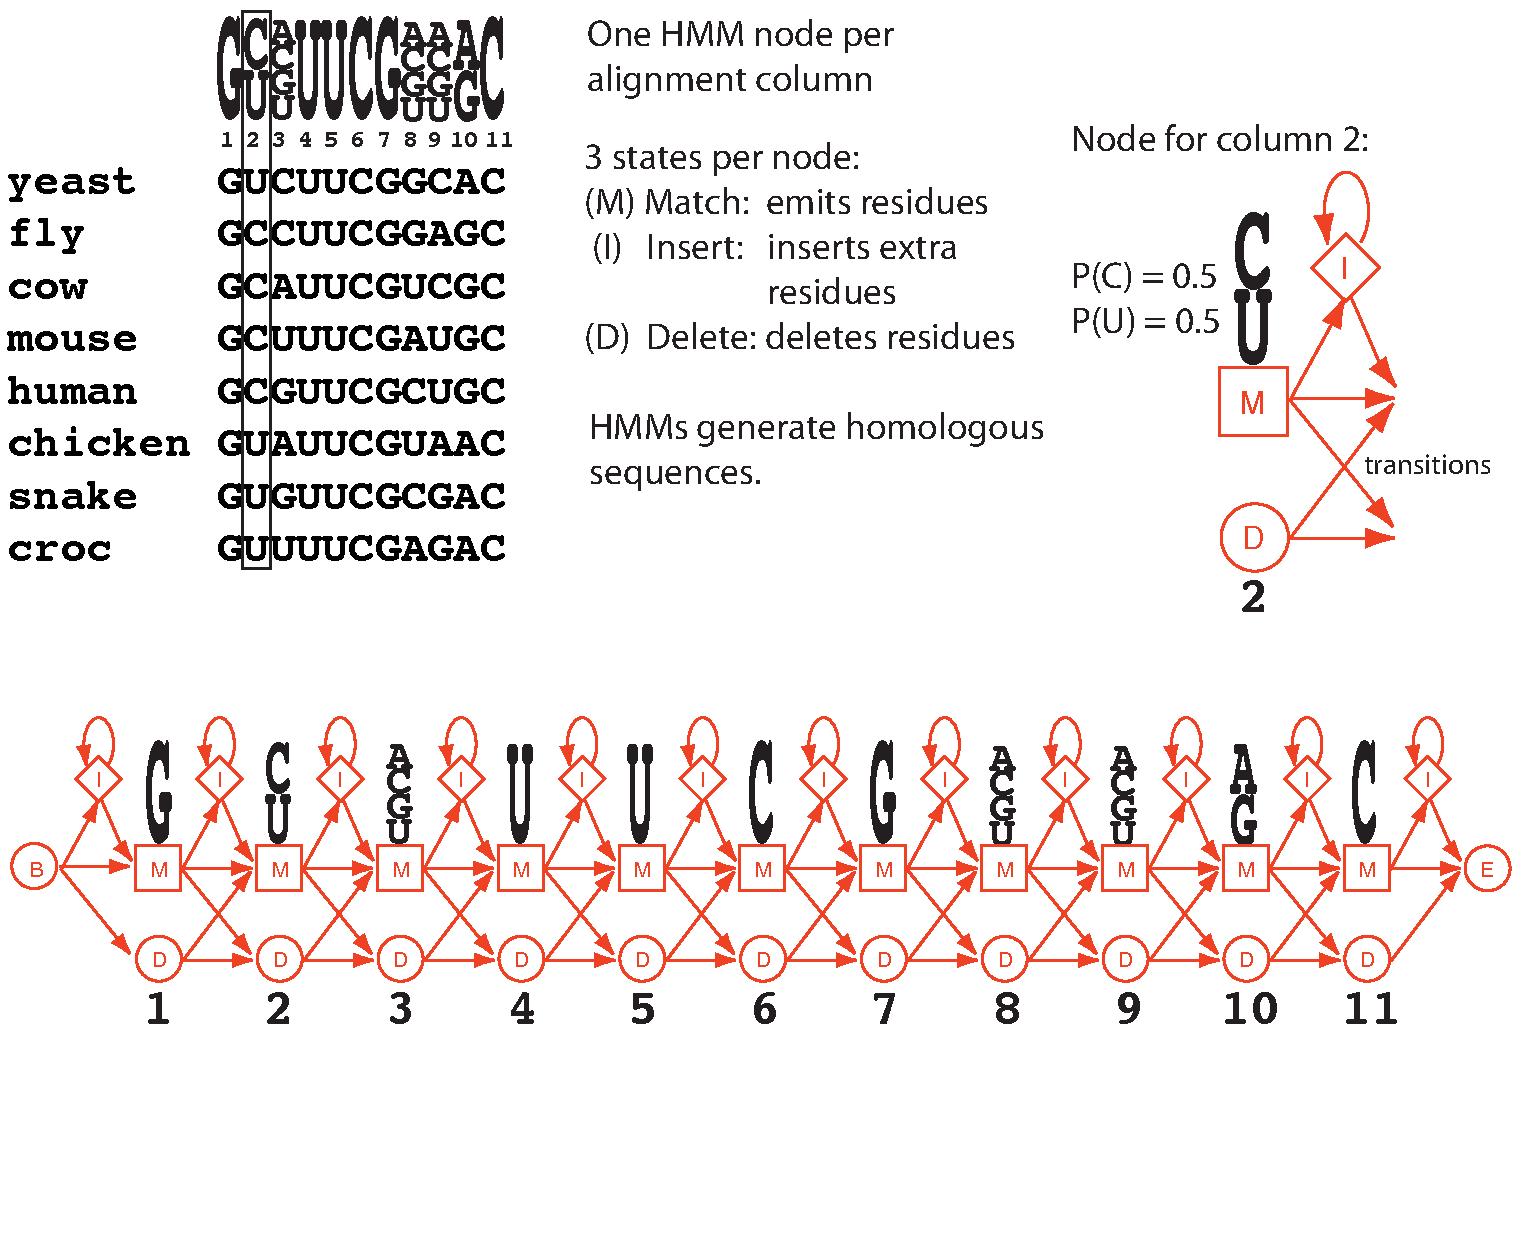
\includegraphics[height=6.625in]{figs/hmm}}

%An HMM generates ``homologous'' sequences.

\end{slide}
%%%%%%%%%%%%%%%%%%%%%%%%%%%%%%%%%%%%%%%%%%%%%%%%%%%%%%%%%%%%%%%
\begin{slide}
\begin{center}
%\textbf{profile HMMs and covariance models}
\textbf{Profile HMMs: sequence family models built from alignments}
\end{center}

\center{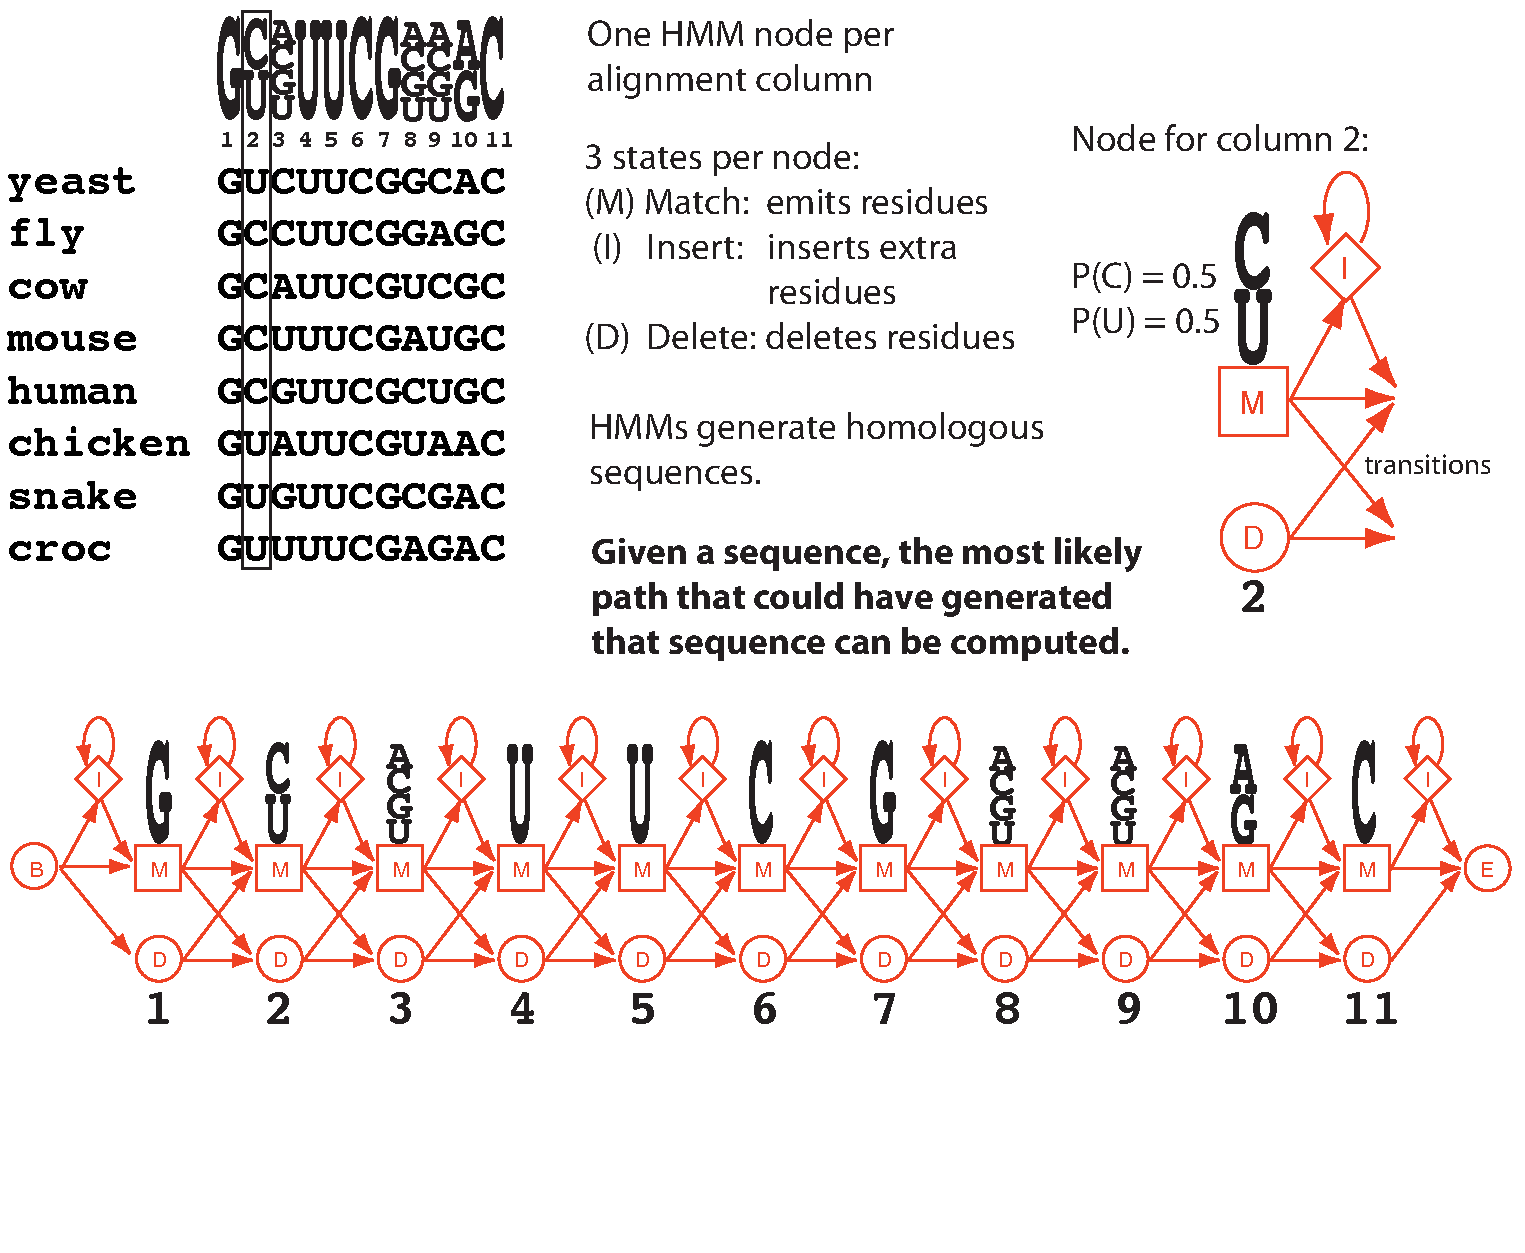
\includegraphics[height=6.625in]{figs/hmm-given}}
\end{slide}
%%%%%%%%%%%%%%%%%%%%%%%%%%%%%%%%%%%%%%%%%%%%%%%%%%%%%%%%%%%%%%%
\begin{slide}
\begin{center}
%\textbf{profile HMMs and covariance models}
\textbf{Profile HMMs: sequence family models built from alignments}
\end{center}

\center{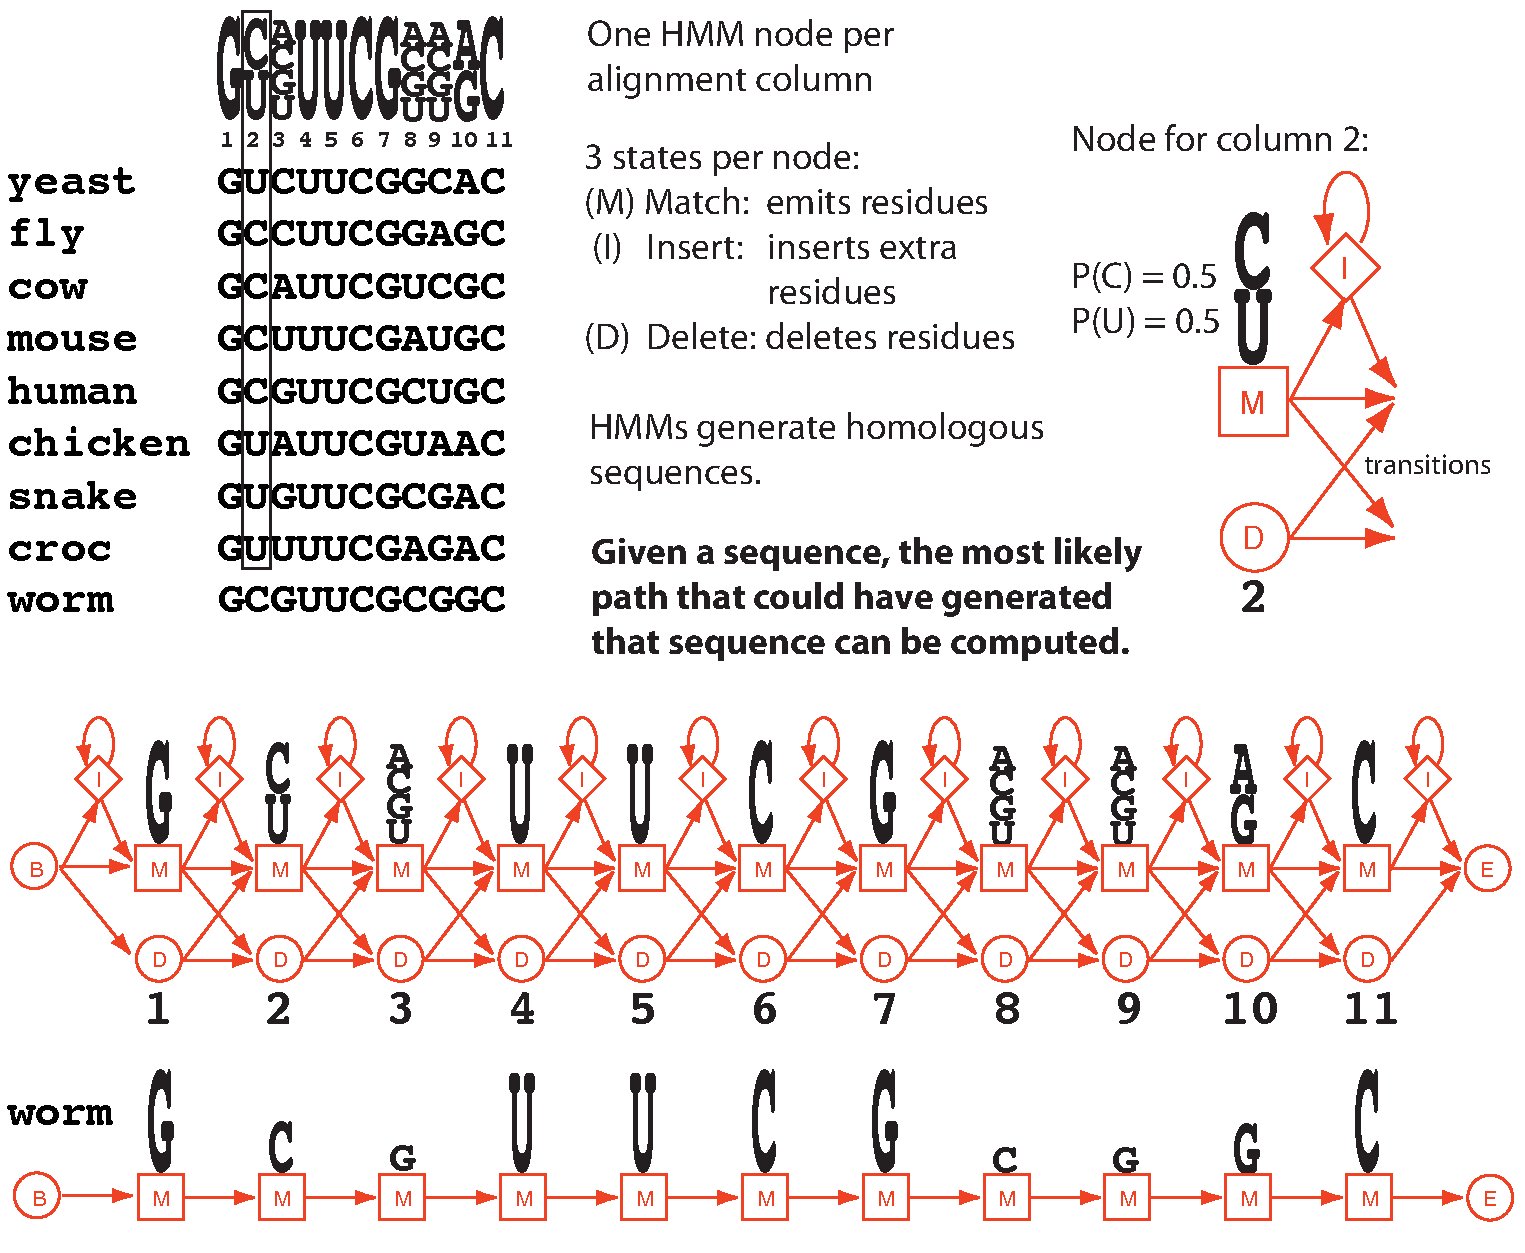
\includegraphics[height=6.625in]{figs/hmm-worm}}
\end{slide}
%%%%%%%%%%%%%%%%%%%%%%%%%%%%%%%%%%%%%%%%%%%%%%%%%%%%%%%%%%%
\begin{slide}
\begin{center}
%\textbf{profile HMMs and covariance models}
\textbf{Profile HMMs: sequence family models built from alignments}
\end{center}

\center{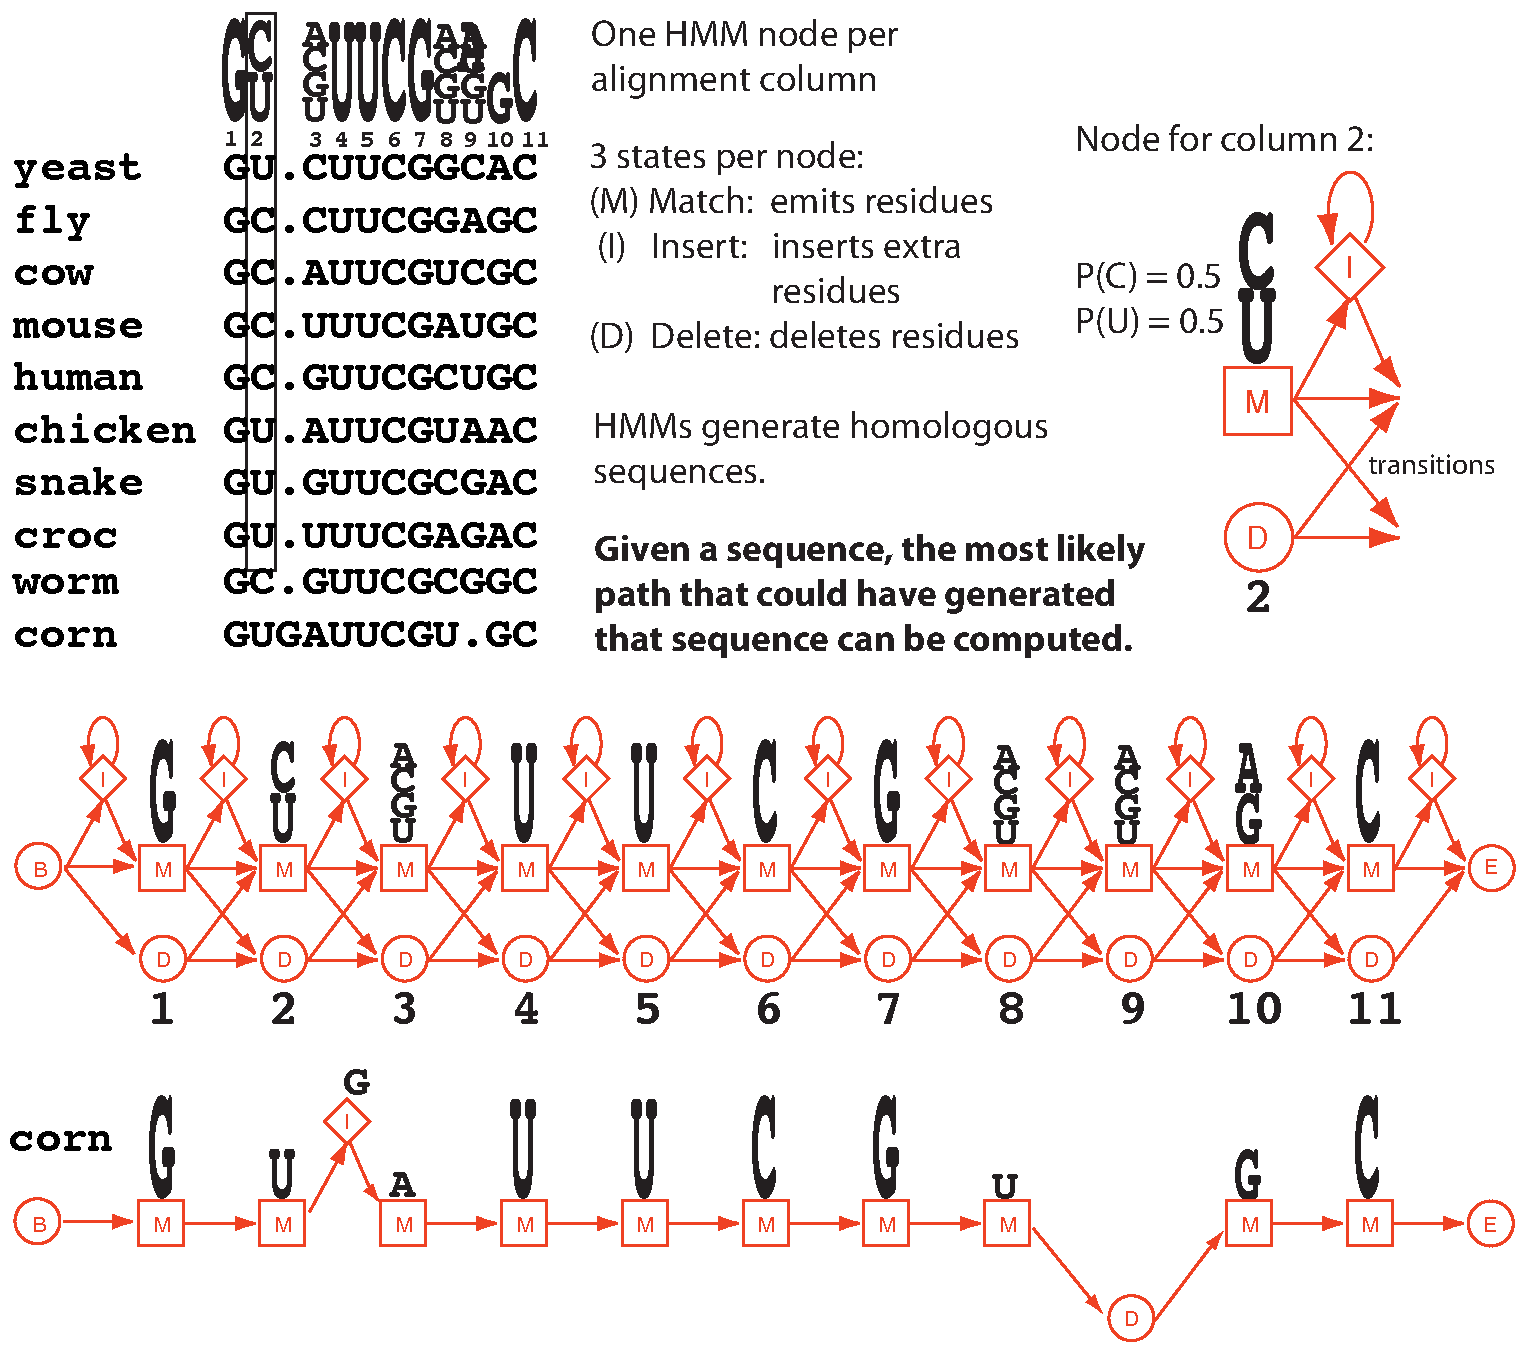
\includegraphics[height=6.625in]{figs/hmm-corn}}
\end{slide}
%%%%%%%%%%%%%%%%%%%%%%%%%%%%%%%%%%%%%%%%%%%%%%%%%%%%%%%%%%%%%%%
\begin{slide}
\begin{center}
%\textbf{profile HMMs and covariance models}
\textbf{Covariance models (CMs) are built \\ from structure-annotated alignments}
\end{center}

\center{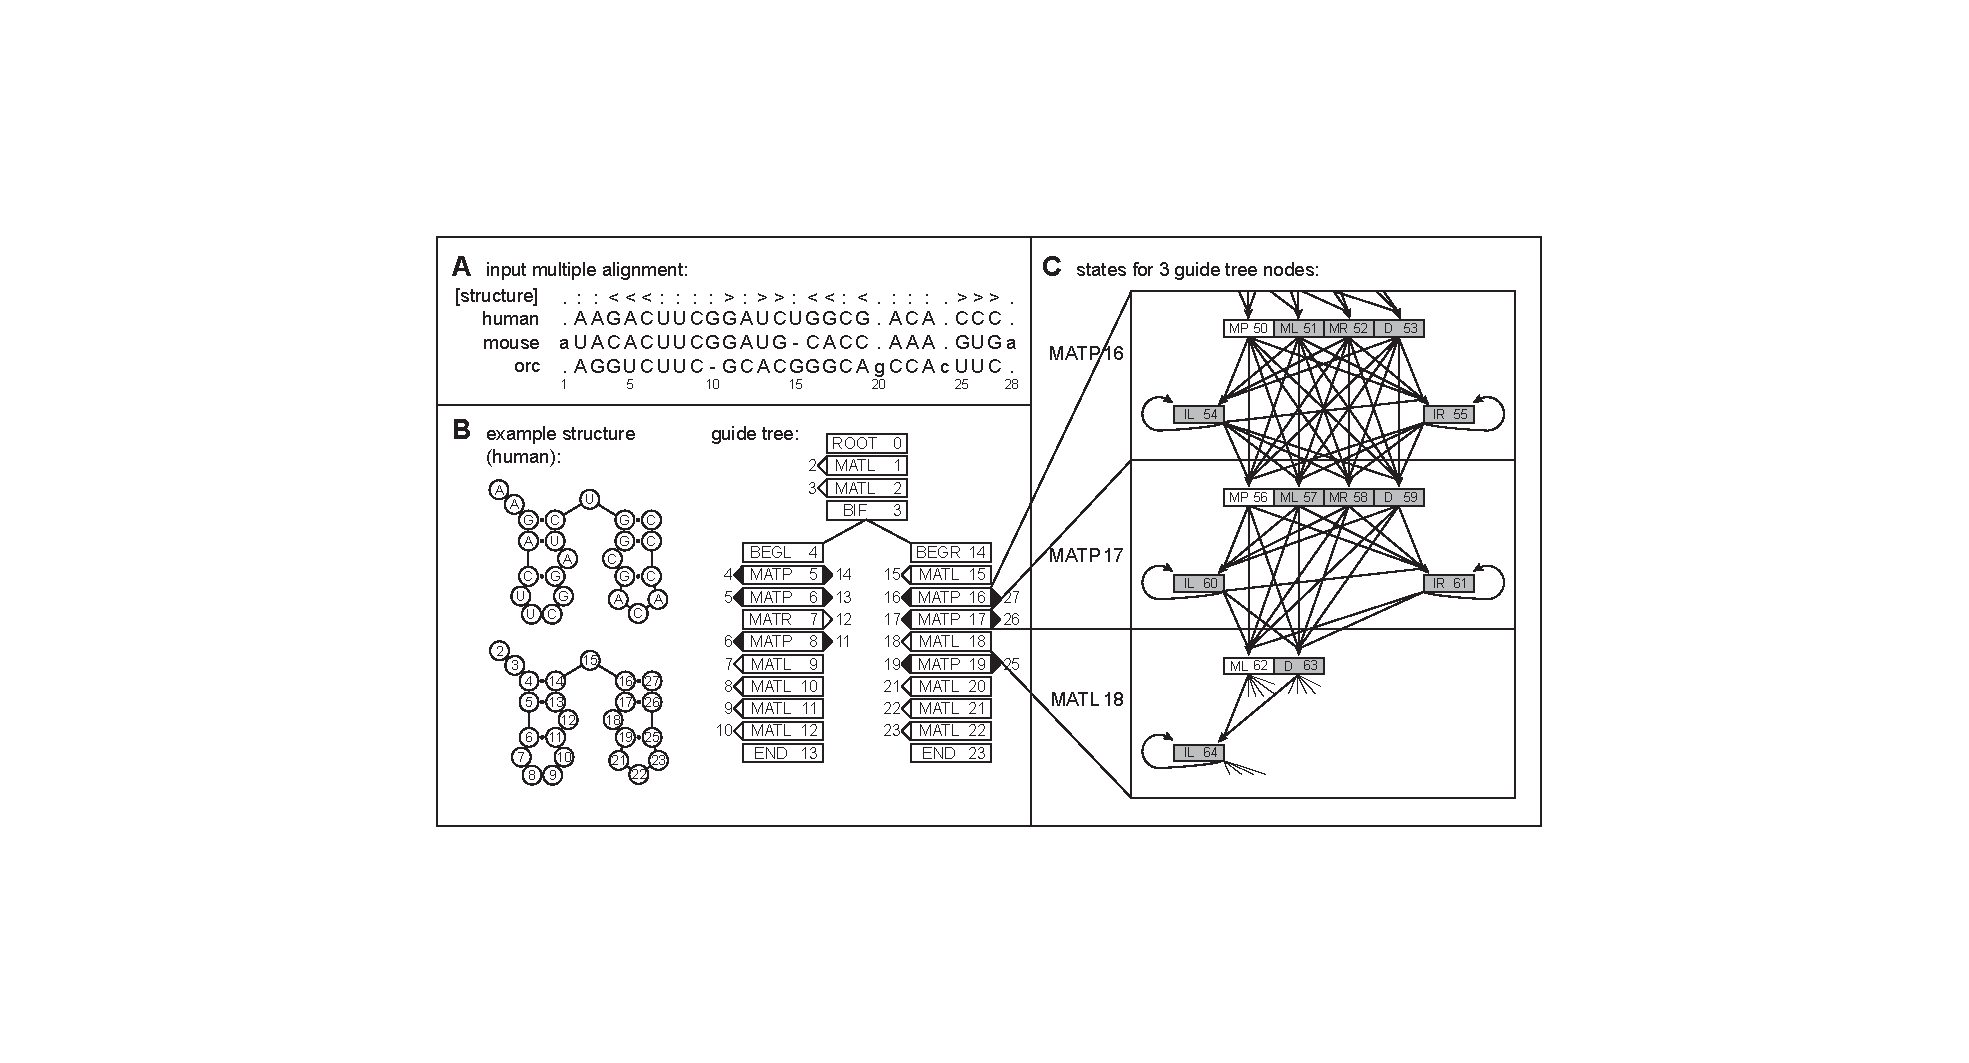
\includegraphics[width=7in]{figs/cmintro_bandcyk}}

\center{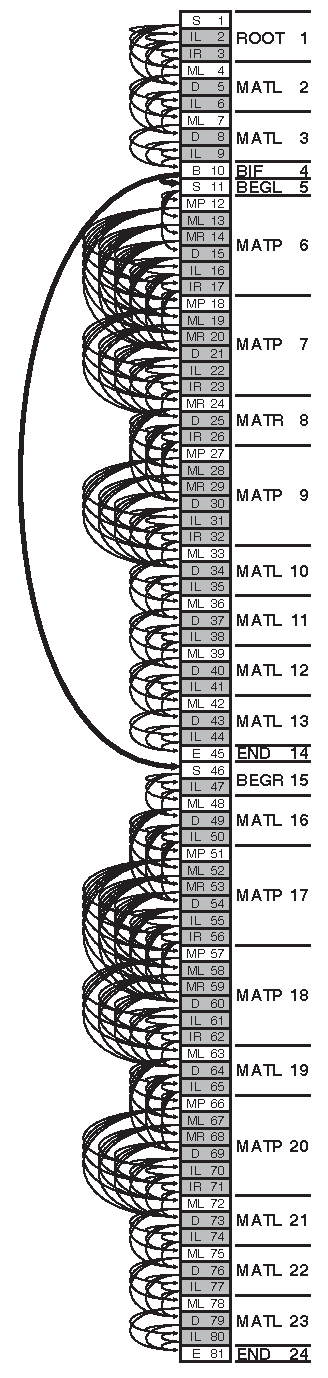
\includegraphics[width=2in,angle=270]{figs/cm-graph-small}}

\vfill

\end{slide}
%%%%%%%%%%%%%%%%%%%%%%%%%%%%%%%%%%%%%%%%%%%%%%%%%%%%%%%%%%%%%%%%%%

%%%%%%%%%%%%%%%%%%%%%%%%%%%%%%%%%%%%%%%%%%%%%%%%%%%%%%%%%%%%%%%
%%%%%%%%%%%%%%%%%%%%%%%%%%%%%%%%%%%%%%%%%%%%%%%%%%%%%%%%%%%%%%%
%%%%%%%%%%%%%%%%%%%%%%%%%%%%%%%%%%%%%%%%%%%%%%%%%%%%%%%%%%%%%%%
%%%%%%%%%%%%%%%%%%%%%%%%%%%%%%%%%%%%%%%%%%%%%%%%%%%%%%%%%%%%%%%
%%%%%%%%%%%%%%%%%%%%%%%%%%%%%%%%%%%%%%%%%%%%%%%%%%%%%%%%%%%%%%%
\begin{slide}
\begin{center}
\textbf{Is the added complexity worth it? \\
  RMARK: a challenging \underline{internal} RNA homology search
  benchmark}

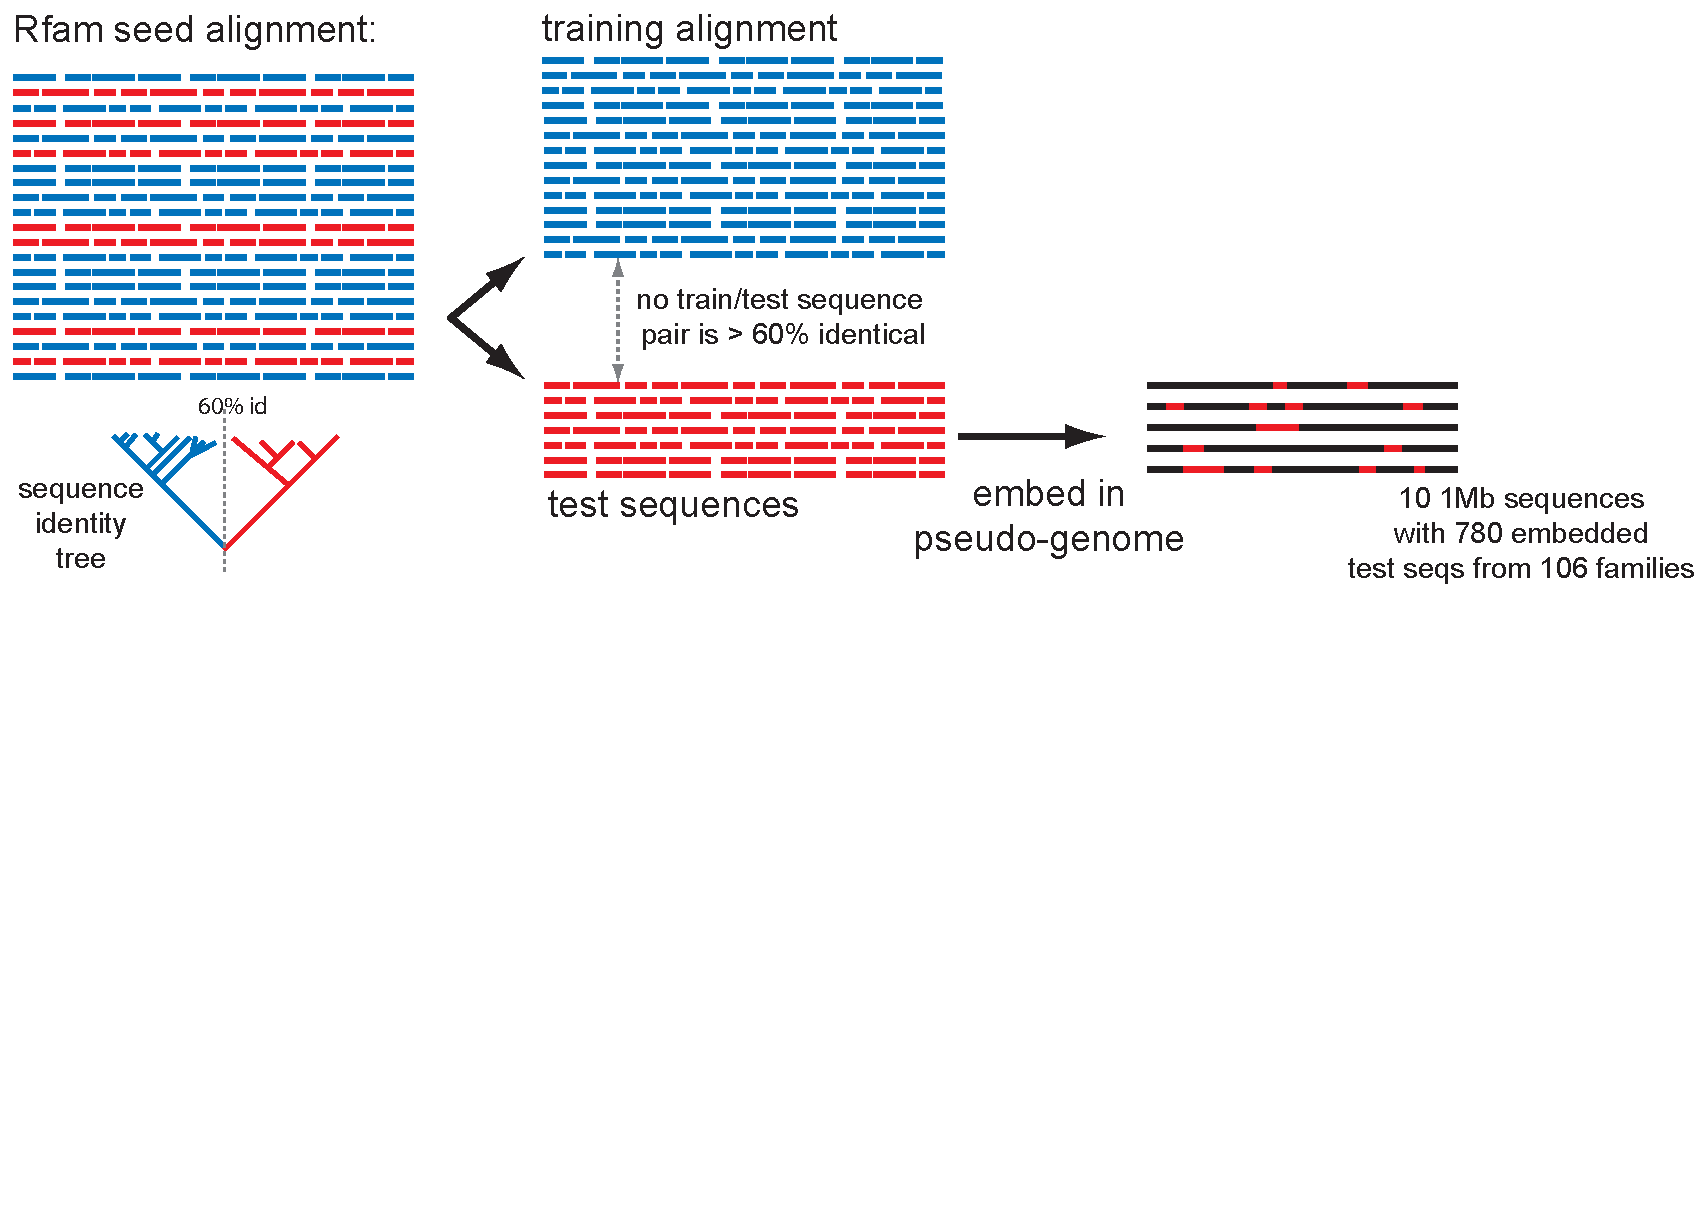
\includegraphics[width=10in]{figs/rmark-tree-1}
\end{center}

\vfill
\end{slide}
%%%%%%%%%%%%%%%%%%%%%%%%%%%%%%%%%%%%%%%%%%%%%%%%%%%%%%%%%%%%%%%%%%%%%%
\begin{slide}
\begin{center}
\textbf{Is the added complexity worth it? \\
  RMARK: a challenging \underline{internal} RNA homology search
  benchmark}

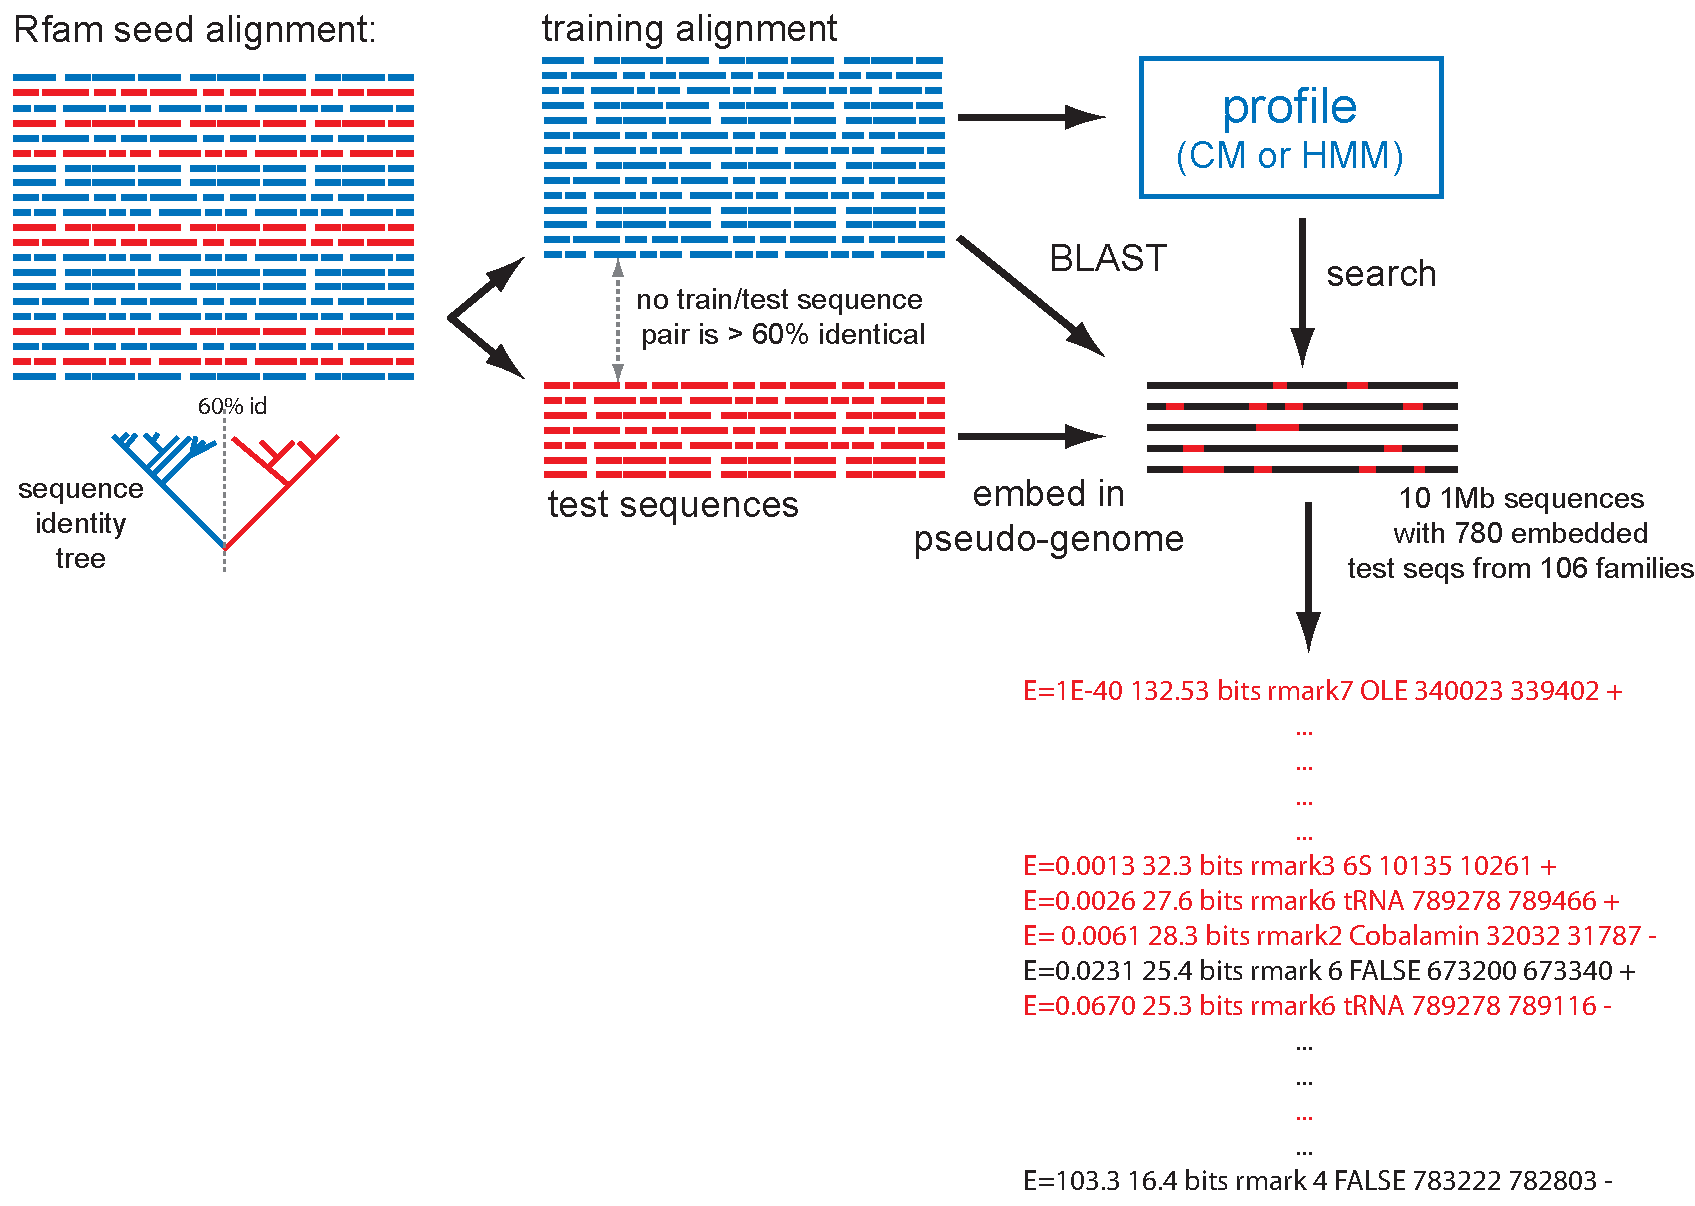
\includegraphics[width=10in]{figs/rmark-tree-2}
\end{center}

\vfill
\end{slide}
%%%%%%%%%%%%%%%%%%%%%%%%%%%%%%%%%%%%%%%%%%%%%%%%%%%%%%%%%%%%%%%
\begin{slide}
\begin{center}

\textbf{Infernal outperforms primary-sequence based methods on our
  benchmark (and others\footnote{Freyhult EK, Bollback JP, Gardner
    PP. Genome Res. 2007 17: 117-125.}, not shown)}

\end{center}
\medskip

\center{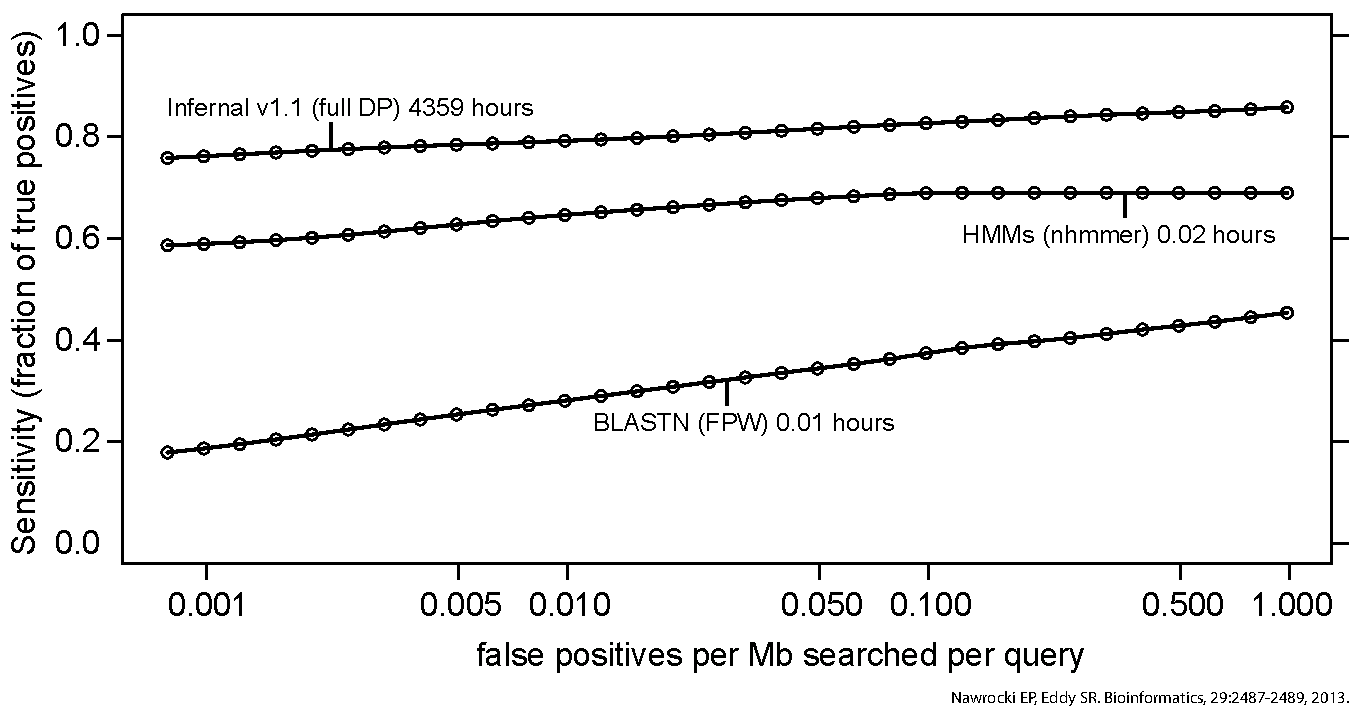
\includegraphics[width=10in]{figs/roc-talk-rcb-2014-1}}

\vfill 
\end{slide}
%%%%%%%%%%%%%%%%%%%%%%%%%%%%%%%%%%%%%%%%%%%%%%%%%%%%%%%%%%%%%%%%%%%%%%
%%%%%%%%%%%%%%%%%%%%%%%%%%%%%%%%%%%%%%%%%%%%%%%%%%%%%%%%%%%%%%%%%%%%%%
\begin{slide}
\begin{center}
\textbf{Outline of talk}

\begin{description}
\item[1.] Motivation: collecting homologs facilitates comparative
  sequence analysis.\\ 1965: Secondary structure determination of
  transfer RNA.
\item[2.] Sequence and sequence+structure profiles
%\item[3.] Benchmarking RNA homology search
\item[\textcolor{red}{3.}] \textcolor{red}{Accelerating RNA homology search}
\item[4.] Implications for Rfam
\item[5.] New features in latest version of Infernal
\end{description}

\end{center}
\vfill
\end{slide}
%%%%%%%%%%%%%%%%%%%%%%%%%%%%%%%%%%%%%%%%%%%%%%%%%%%%%%%%%%%%%%%%%%%%
\begin{slide}
\begin{center}
\large
\textbf{Filter target database using profile HMMs\footnote{Weinberg,
    Ruzzo, RECOMB, 243-251, 2004; Weinberg, Ruzzo, Bioinformatics,
    22(1) 35-39 2006.}}
\end{center}

\center{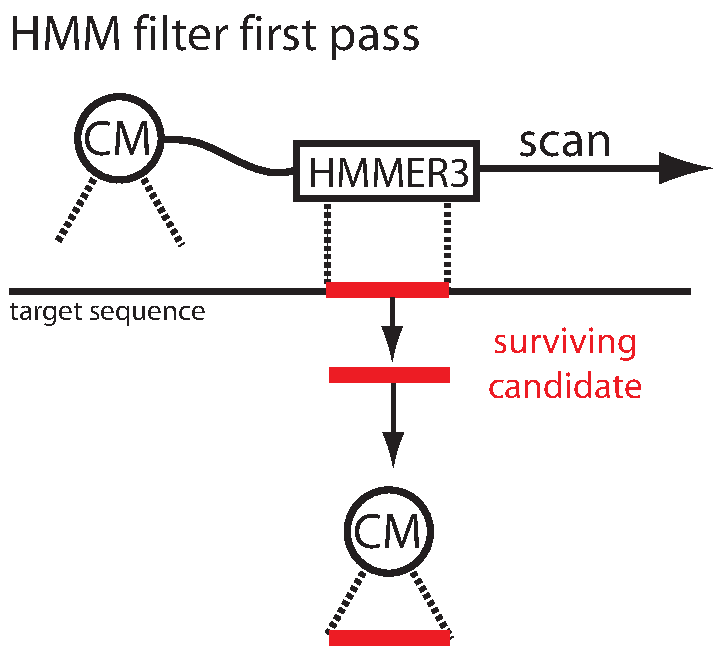
\includegraphics[height=4in]{figs/filter-2014-1}}

\vfill
\end{slide}
%%%%%%%%%%%%%%%%%%%%%%%%%%%%%%%%%%%%%%%%%%%%%%%%%%%%%%%%%%%%%%%%%%%%%%%%%%
\begin{slide}
\begin{center}
\large
\textbf{Filter target database using profile HMMs\footnote{Weinberg,
    Ruzzo, RECOMB, 243-251, 2004; Weinberg, Ruzzo, Bioinformatics,
    22(1) 35-39 2006.}}
\end{center}

\center{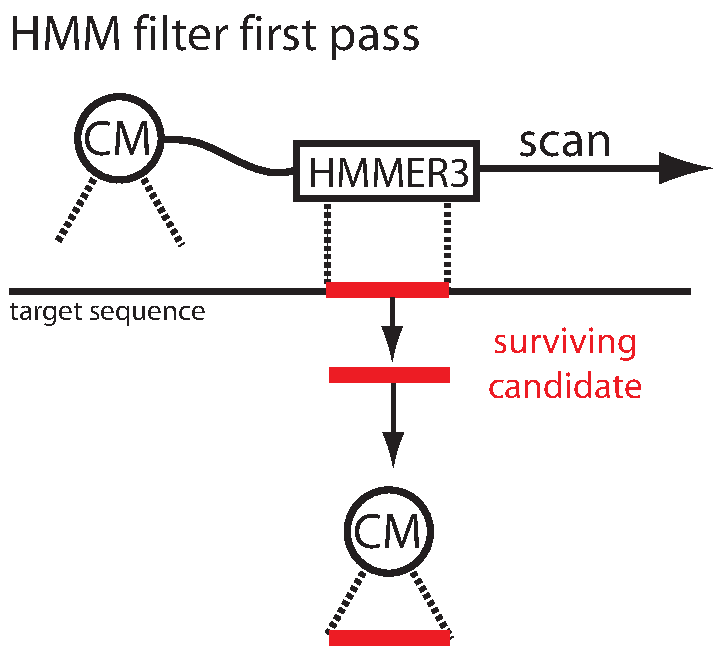
\includegraphics[height=4in]{figs/filter-2014-1}}

\begin{itemize}
\item Even if we filter out 99\% of the database (for up to 100X
  acceleration), searches will still be too slow.
\item CM step needs to be accelerated. 
\end{itemize}

\vfill
\end{slide}
%%%%%%%%%%%%%%%%%%%%%%%%%%%%%%%%%%%%%%%%%%%%%%%%%%%%%%%%%%%%%%%%%%%%%%%%%%
%\begin{slide}
%\begin{center}
%
%\textbf{Accelerating CM alignment step 1: \\ align sequence with HMM}
%
%\includegraphics[height=6in]{figs/hmm_alignment2_layer2}
%\end{center}
%
%\vfill
%\end{slide}
%%%%%%%%%%%%%%%%%%%%%%%%%%%%%%%%%%%%%
%%%%%%%%%%%%%%%%%%%%%%%%%%%%%%%%%%%%%%%%%%%%%%%%%%%%%%%%%%%%%%%%%%%%%%%%%%
\begin{slide}
\begin{center}

%\textbf{Accelerating CM alignment step 2: \\ HMM posterior decoding to
%  get confidence estimates}
\textbf{Accelerating CM alignment step 1: \\ HMM posterior decoding to
  get confidence estimates}

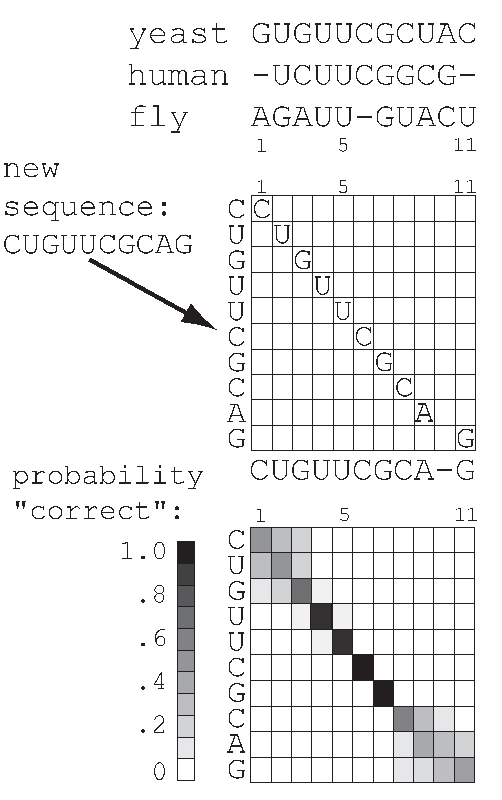
\includegraphics[height=6in]{figs/hmm_alignment2_layer3}
\end{center}

\vfill
\end{slide}
%%%%%%%%%%%%%%%%%%%%%%%%%%%%%%%%%%%%%
\begin{slide}
\begin{center}

\textbf{Accelerating CM alignment step 2: \\ use HMM alignment
  confidence to constrain CM alignment\footnote{M. P. Brown. Proc. Int. Conf. ISMB, 8:57–66, 2000.}}
\end{center}
\medskip
\small
%\begin{itemize}
%\item
%\textbf{main idea:} eliminate potential alignments the HMM tells us are very improbable
%\end{itemize}
\begin{center}
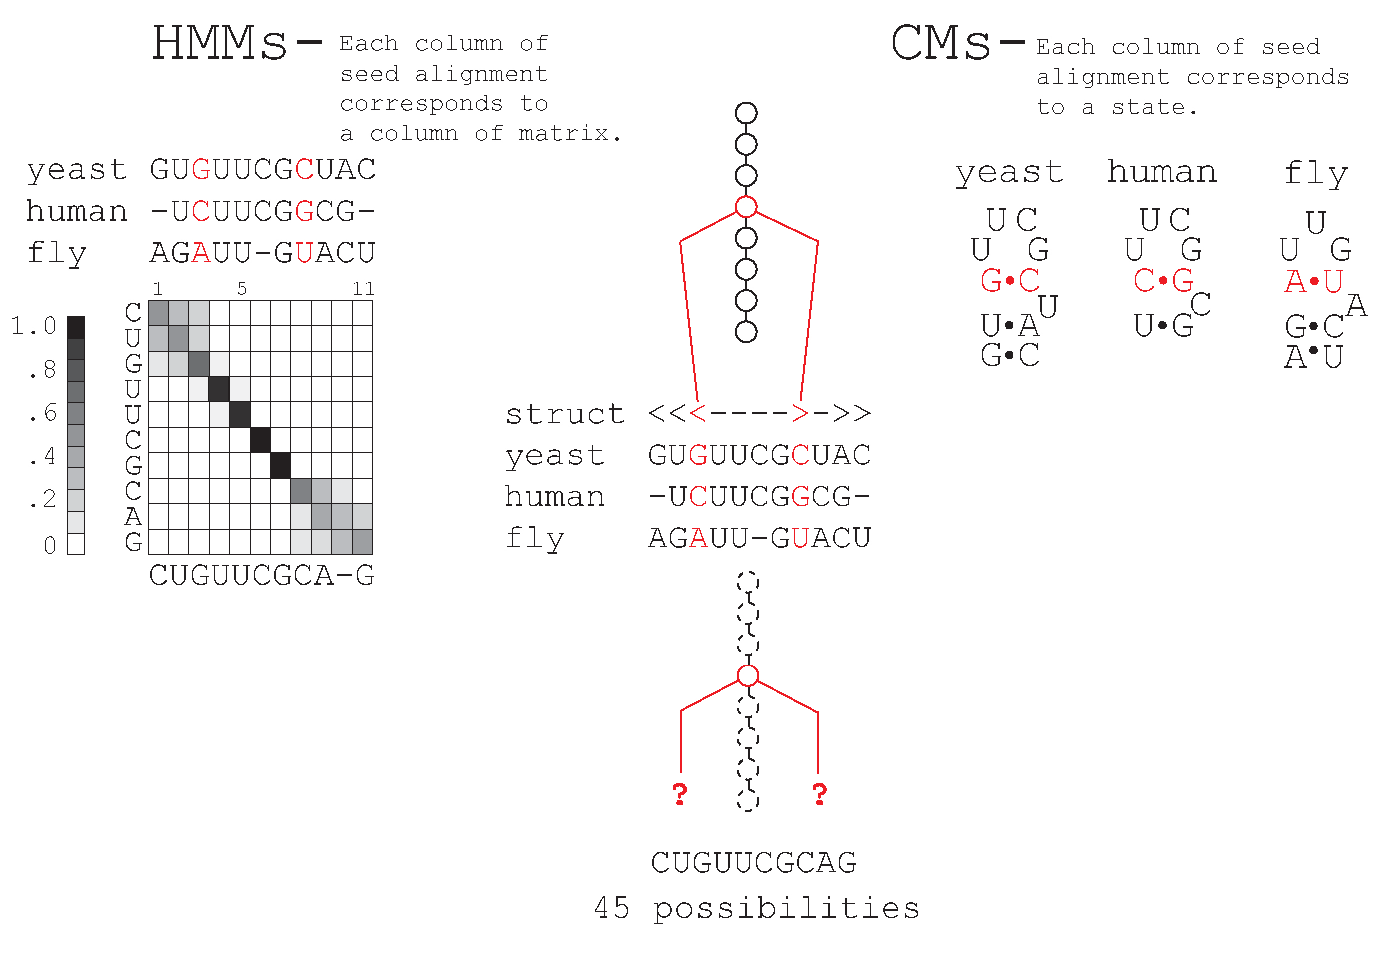
\includegraphics[width=8in]{figs/post_hmm_to_cm_map2_layer14}
\end{center}
\vfill
\end{slide}
%%%%%%%%%%%%%%%%%%%%%%%%%%%%%%%%%%%%%%%%%%%%%%%%%%%%%%%%%%%%%%%%%%%%%%
\begin{slide}
\begin{center}

\textbf{Accelerating CM alignment step 2: \\ use HMM alignment
  confidence to constrain CM alignment\footnote{M. P. Brown. Proc. Int. Conf. ISMB, 8:57–66, 2000.}}
\end{center}
\medskip
\small
%\begin{itemize}
%\item
%\textbf{main idea:} eliminate potential alignments the HMM tells us are very improbable
%\end{itemize}
\begin{center}
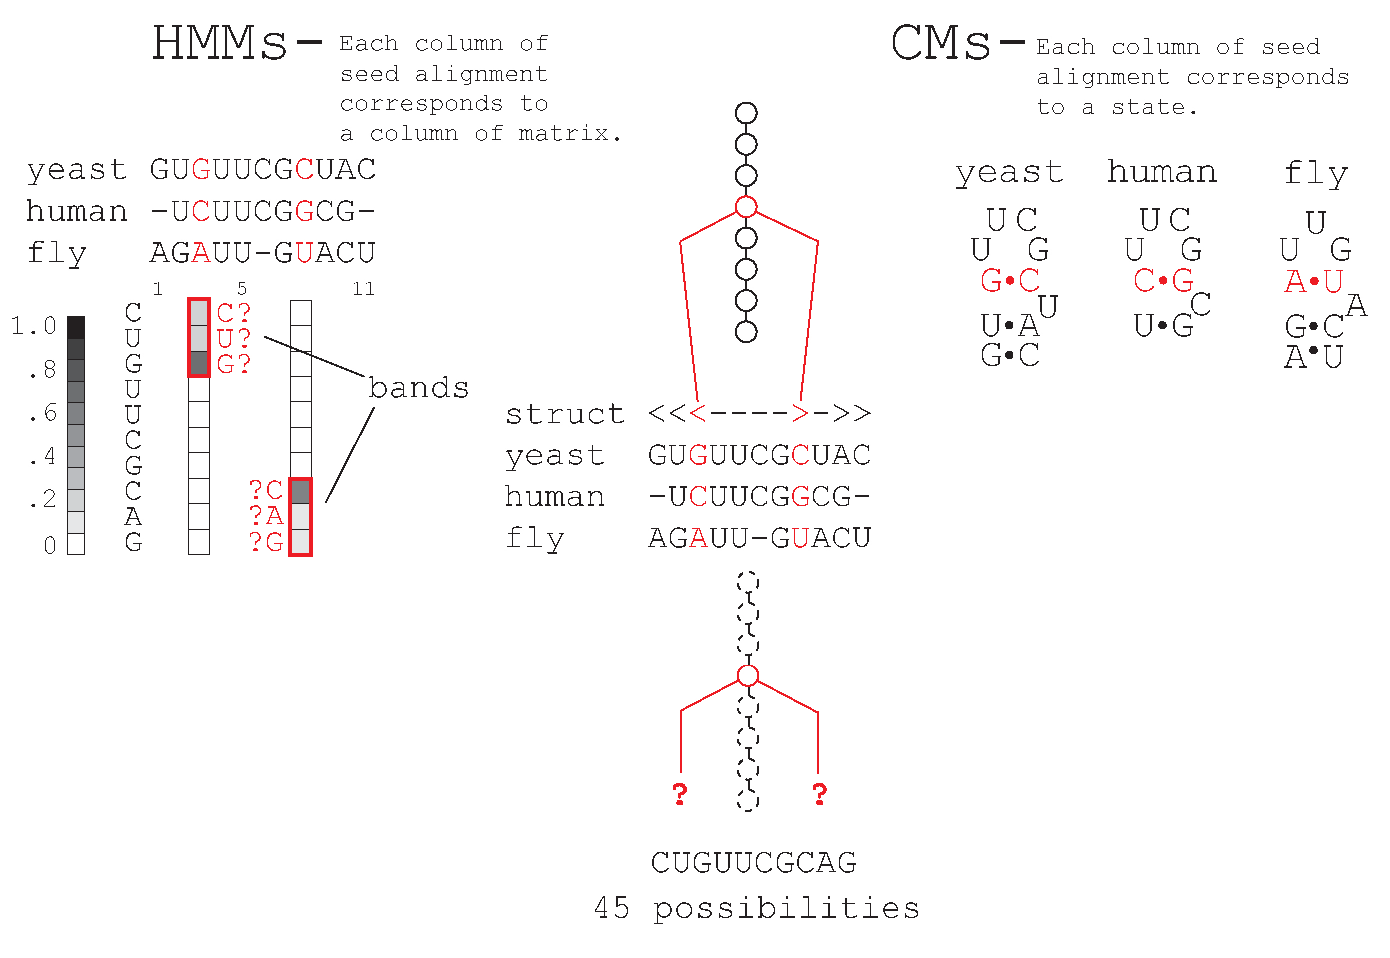
\includegraphics[width=8in]{figs/post_hmm_to_cm_map2_layer15}
\end{center}
\vfill
\end{slide}
%%%%%%%%%%%%%%%%%%%%%%%%%%%%%%%%%%%%%%%%%%%%%%%%%%%%%%%%%%%%%%%%%%%%%%%%%%
\begin{slide}
\begin{center}

\textbf{Accelerating CM alignment step 3: \\ use HMM alignment
  confidence to constrain CM alignment\footnote{M. P. Brown. Proc. Int. Conf. ISMB, 8:57–66, 2000.}}
\end{center}
\medskip
\small
%\begin{itemize}
%\item
%\textbf{main idea:} eliminate potential alignments the HMM tells us are very improbable
%\end{itemize}
\begin{center}
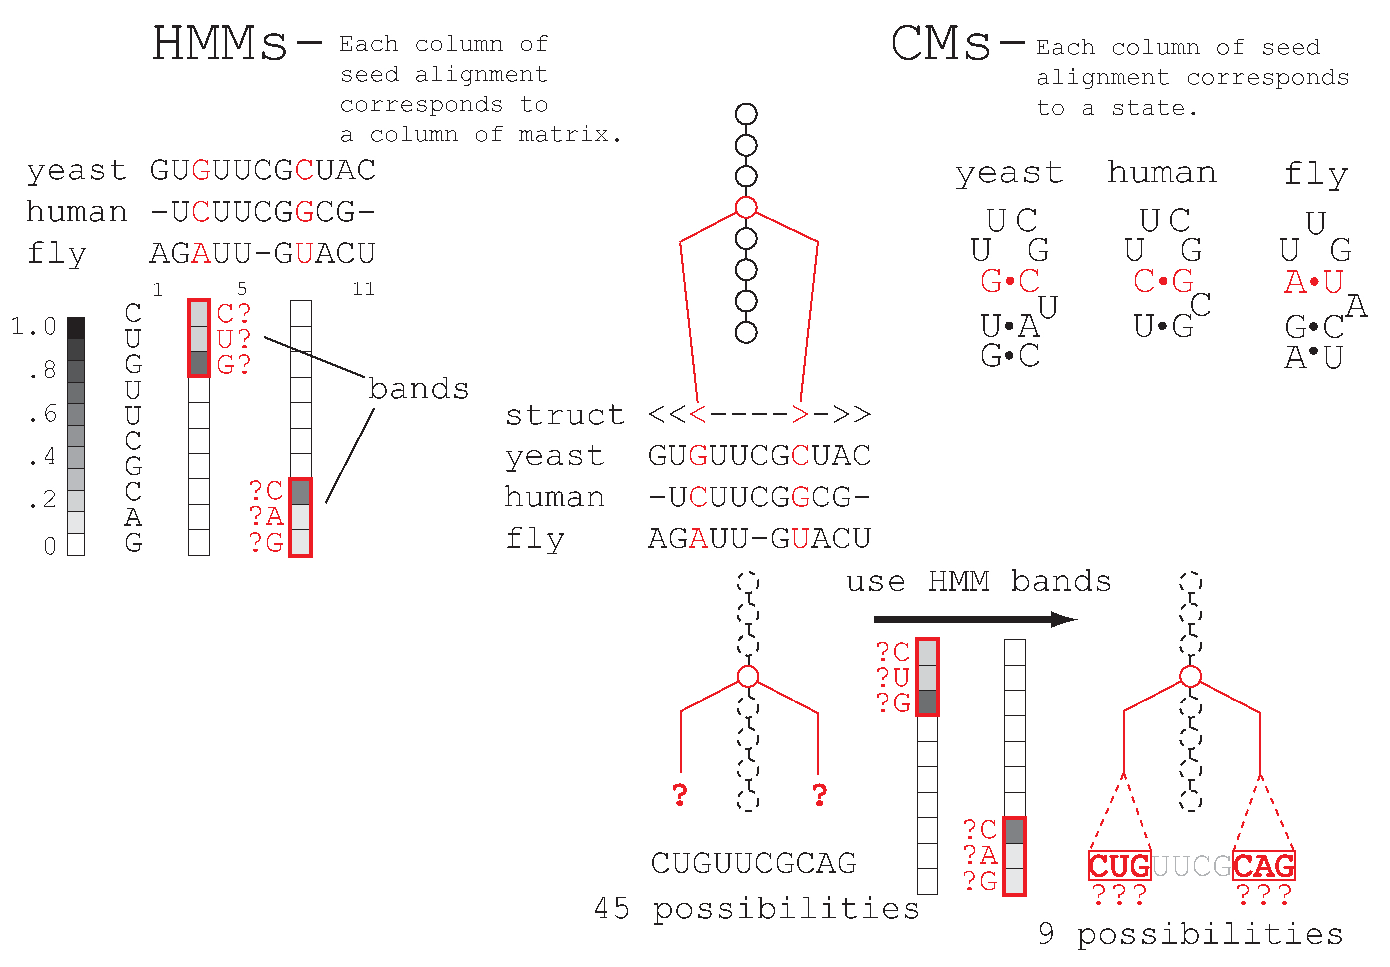
\includegraphics[width=8in]{figs/post_hmm_to_cm_map2_layer16}
\end{center}
\vfill
\end{slide}
%%%%%%%%%%%%%%%%%%%%%%%%%%%%%%%%%%%%%%%%%%%%%%%%%%%%%%%%%%%%%%%%%%%%%%
%\begin{slide}
%\center{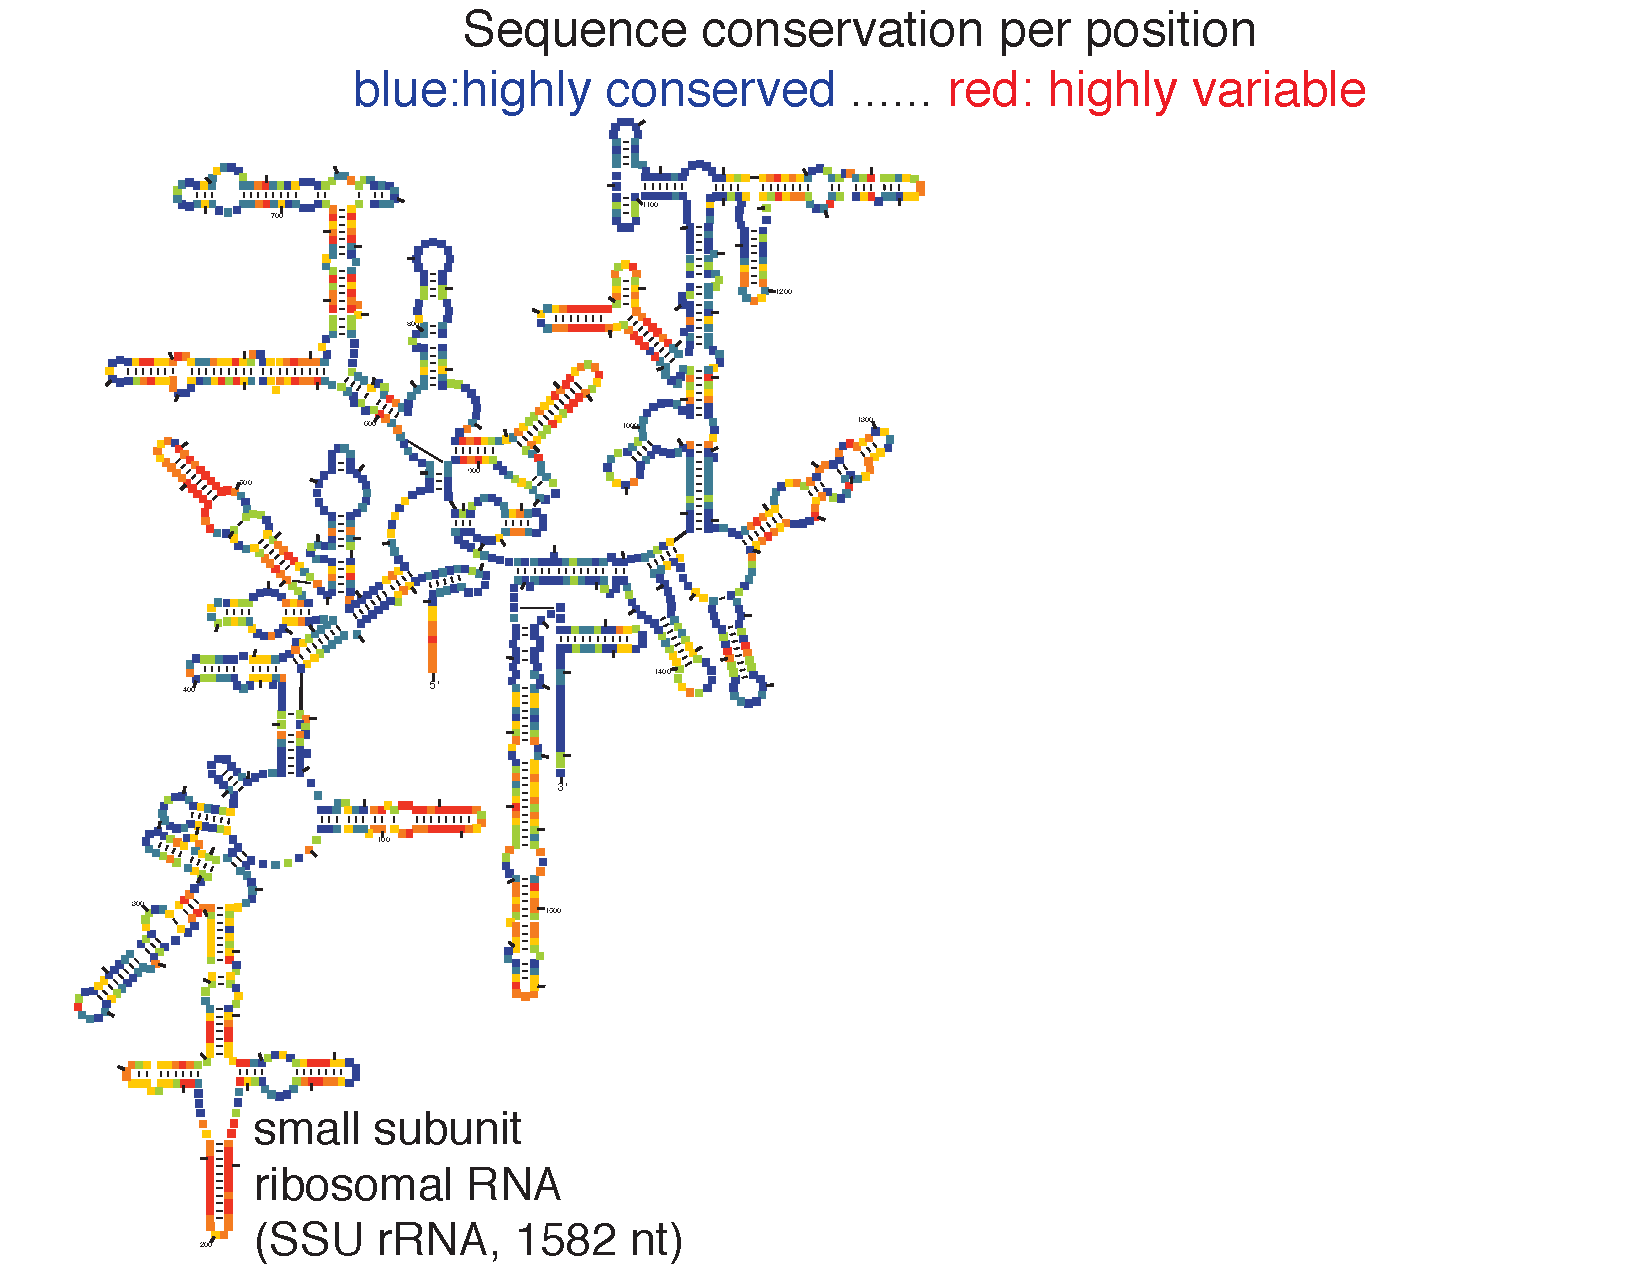
\includegraphics[width=10.5in]{figs/16s-5s-trna-info-16sonly}}
%\end{slide}
%%%%%%%%%%%%%%%%%%%%%%%%%%%%%%%%%%%%%%%%%%%%%%%%%%%%%%%%%%%%%%%%%%%%%%
\begin{slide}
\center{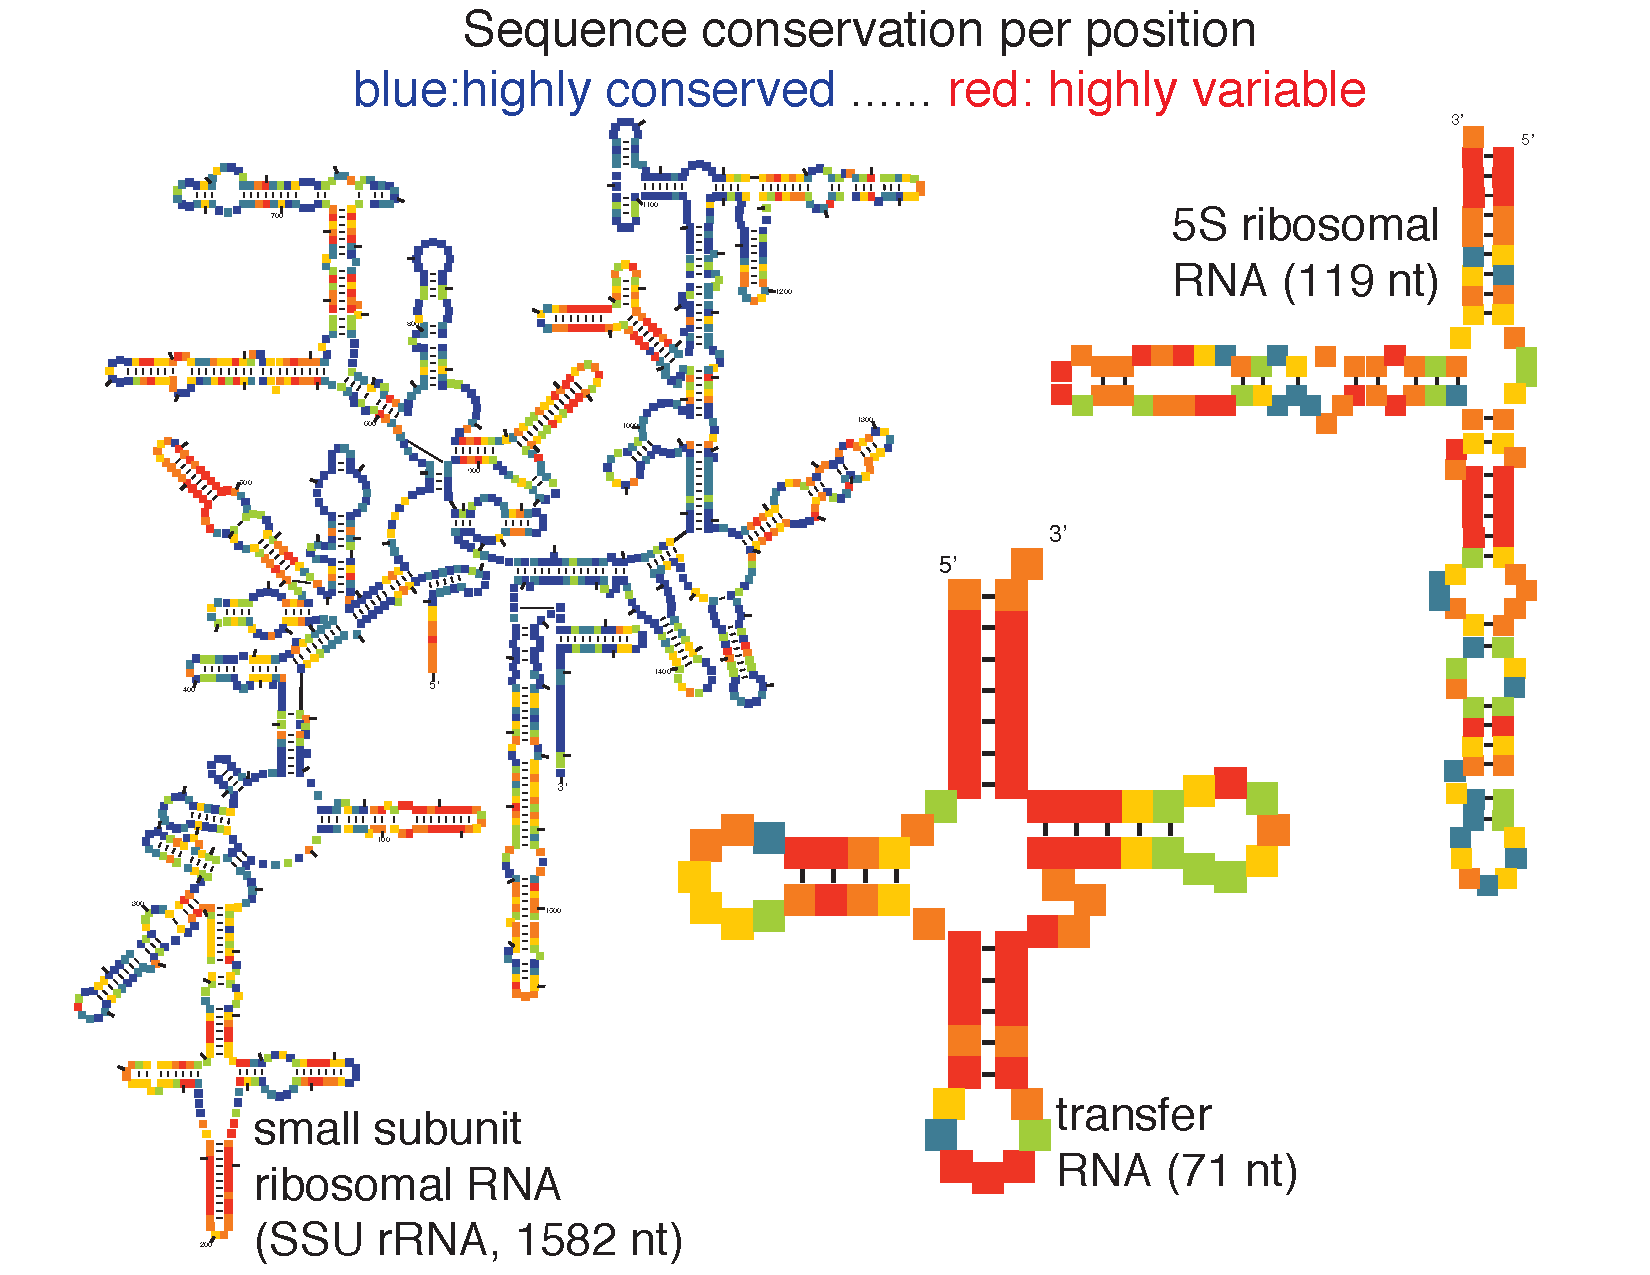
\includegraphics[width=10.5in]{figs/16s-5s-trna-info}}
\end{slide}
%%%%%%%%%%%%%%%%%%%%%%%%%%%%%%%%%%%%%%%%%%%%%%%%%%%%%%%%%%%%%%%%%%%%
\begin{slide}
\begin{center}
\large
\textbf{Use HMMs as filters and to constrain CM alignment}
\end{center}

\center{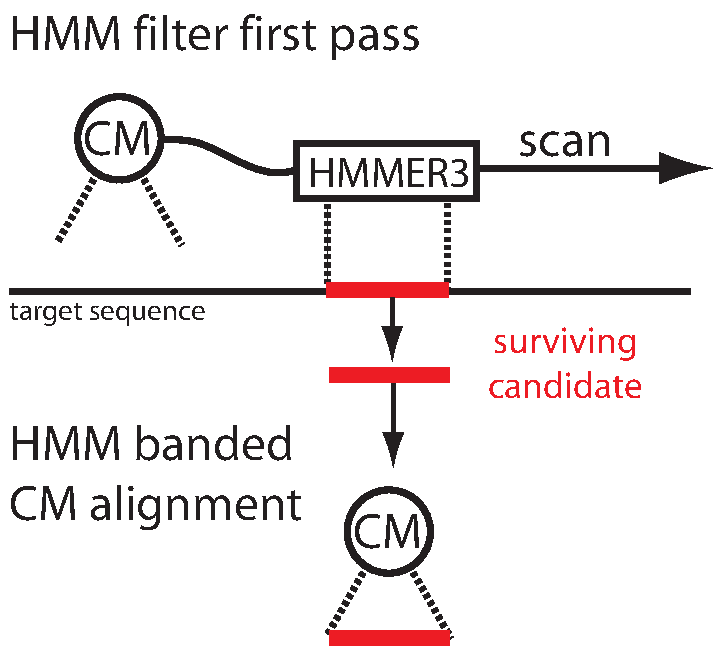
\includegraphics[height=5in]{figs/filter-2014-2}}

\vfill
\end{slide}
%%%%%%%%%%%%%%%%%%%%%%%%%%%%%%%%%%%%%%%%%%%%%%%%%%%%%%%%%%%%%%%%%%%%%%%%%%
\begin{slide}
\begin{center}

\textbf{HMM-based acceleration makes Infernal 10,000 times faster}

\end{center}
\medskip

\center{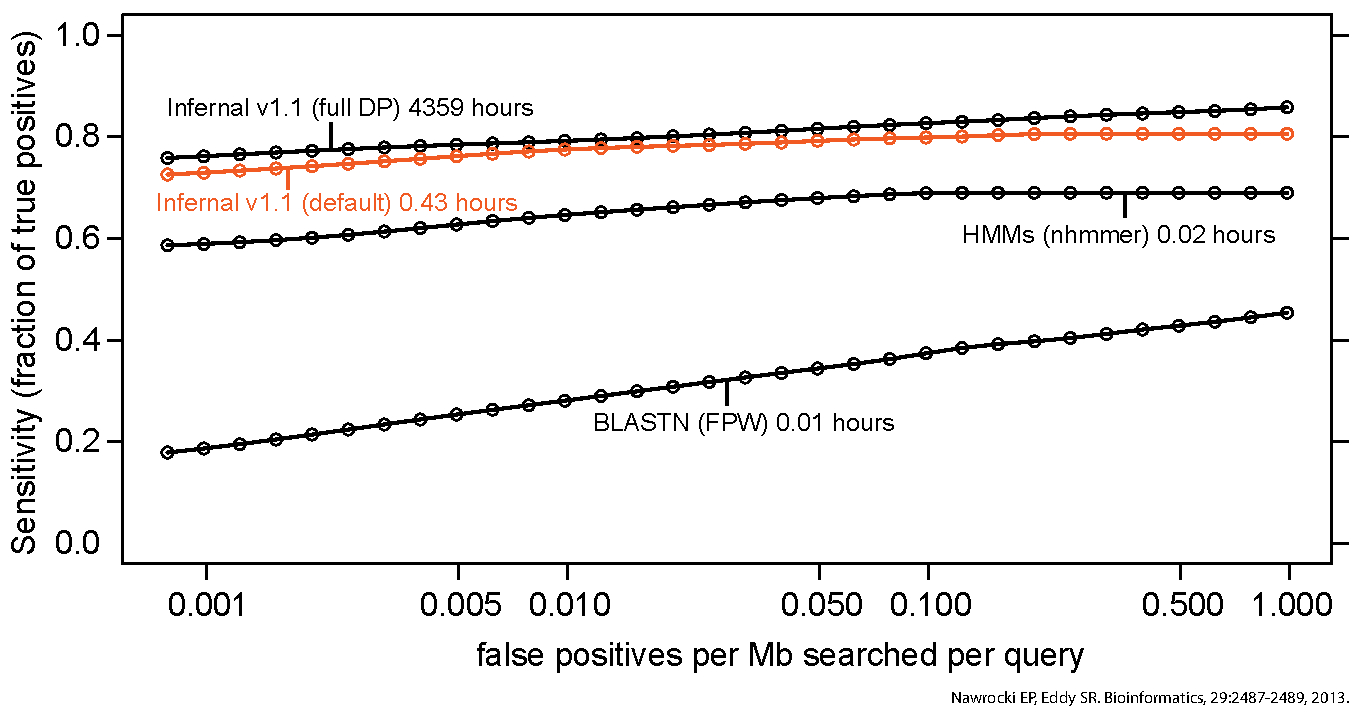
\includegraphics[width=10in]{figs/roc-talk-rcb-2014-2}}

\vfill 
\end{slide}


%%%%%%%%%%%%%%%%%%%%%%%%%%%%%%%%%%%%%%%%%%%%%%%%%%%%%%%%%%%%%%%%%%%%%%
%%%%%%%%%%%%%%%%%%%%%%%%%%%%%%%%%%%%%%%%%%%%%%%%%%%%%%%%%%%%%%%%%%%%%%
\begin{slide}
\begin{center}
\textbf{Outline of talk}

\begin{description}
\item[1.] Motivation: collecting homologs facilitates comparative
  sequence analysis.\\ 1965: Secondary structure determination of
  transfer RNA.
\item[2.] Sequence and sequence+structure profiles
%\item[3.] Benchmarking RNA homology search
\item[3.] Accelerating RNA homology search
\item[\textcolor{red}{4.}] \textcolor{red}{Implications for Rfam}
\item[5.] New features in latest version of Infernal
\end{description}

\end{center}
\vfill
\end{slide}
%%%%%%%%%%%%%%%%%%%%%%%%%%%%%%%%%%%%%%%%%%%%%%%%%%%%%%%%%%%%%%%%%%%%%%%%%%%
\begin{slide}
\begin{center}

\textbf{Rfam used BLAST filters from 2003 to 2012}

\end{center}

\begin{itemize}
\item Rfam includes $>$ 2400 RNA families, each represented by an
  alignment, CM and set of predicted homologs in a large database (Rfamseq).
\end{itemize}

\center{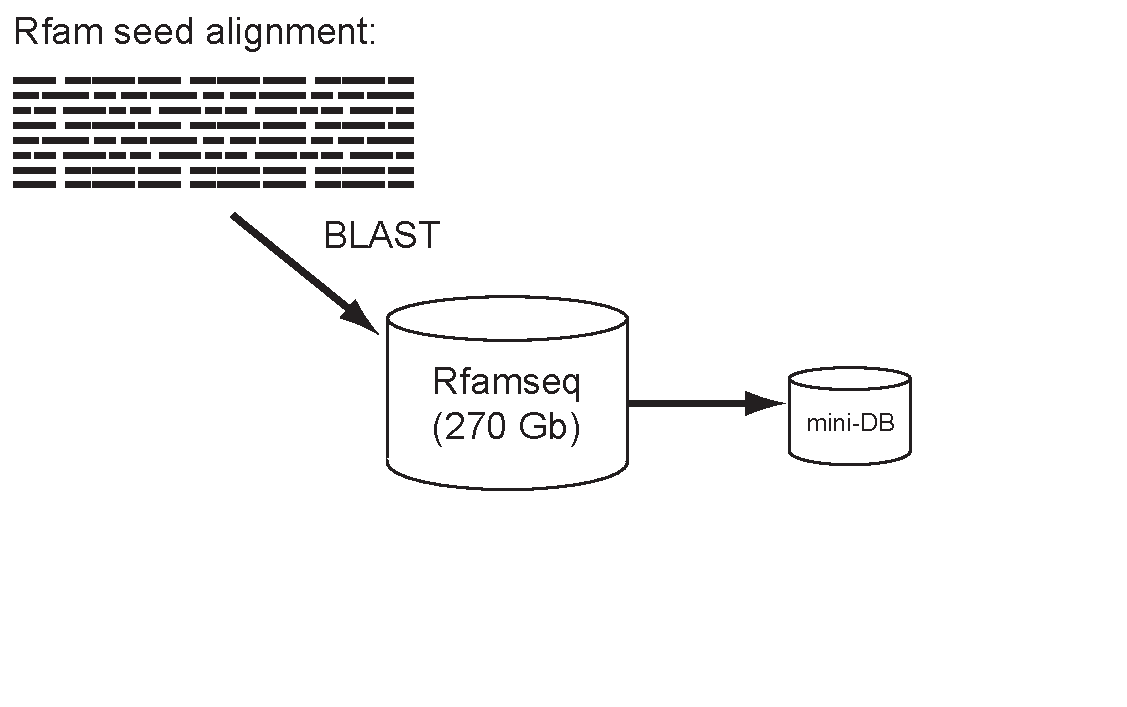
\includegraphics[width=8in]{figs/rfam-search-1}}

\vfill
\end{slide}
%%%%%%%%%%%%%%%%%%%%%%%%%%%%%%%%%%%%%%%%%%%%%%%%%%%%%%%%%%%%%%%%%%%%%%
\begin{slide}
\begin{center}

\textbf{Rfam used BLAST filters from 2003 to 2012}

\end{center}

\begin{itemize}
\item Rfam includes $>$ 2000 RNA families, each represented by an
  alignment, CM and set of predicted homologs in a large database (Rfamseq).
\end{itemize}

\center{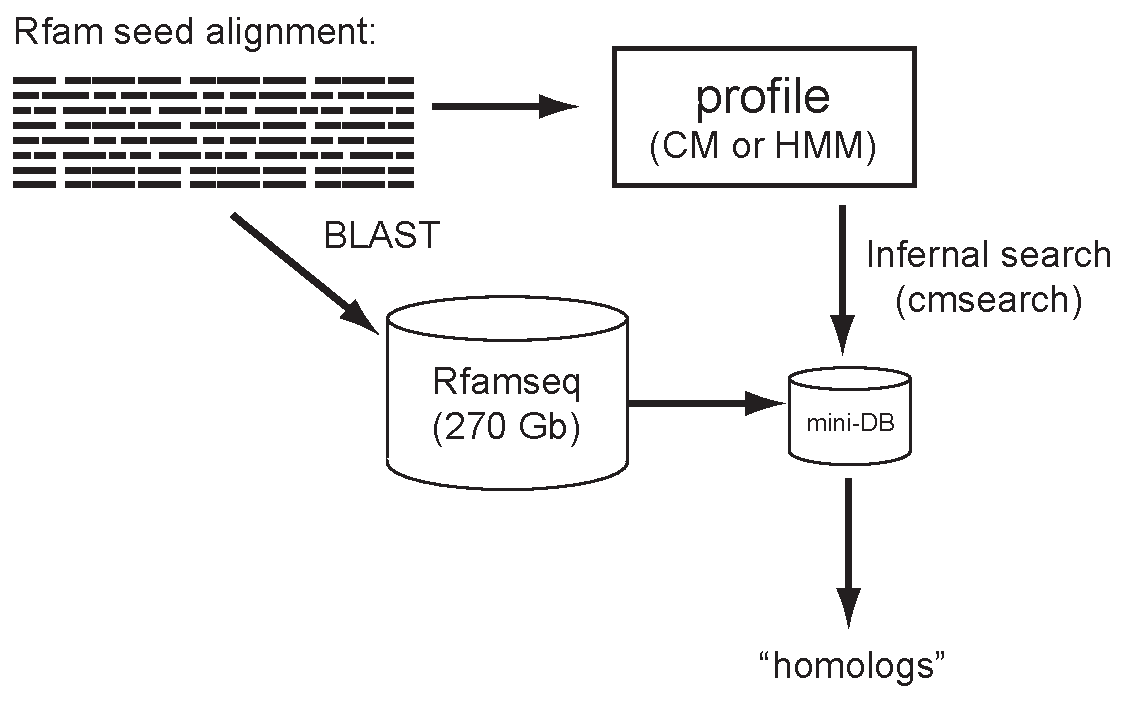
\includegraphics[width=8in]{figs/rfam-search-2}}

\vfill
\end{slide}
%%%%%%%%%%%%%%%%%%%%%%%%%%%%%%%%%%%%%%%%%%%%%%%%%%%%%%%%%%%%%%%%%%%%%%
\begin{slide}
\begin{center}

\textbf{Rfam 12.0 (2014)\footnote{Nawrocki, Burge et. al, NAR 43:D130-D137, 2015.}, 
first release without BLAST filtering}
\end{center}

\center{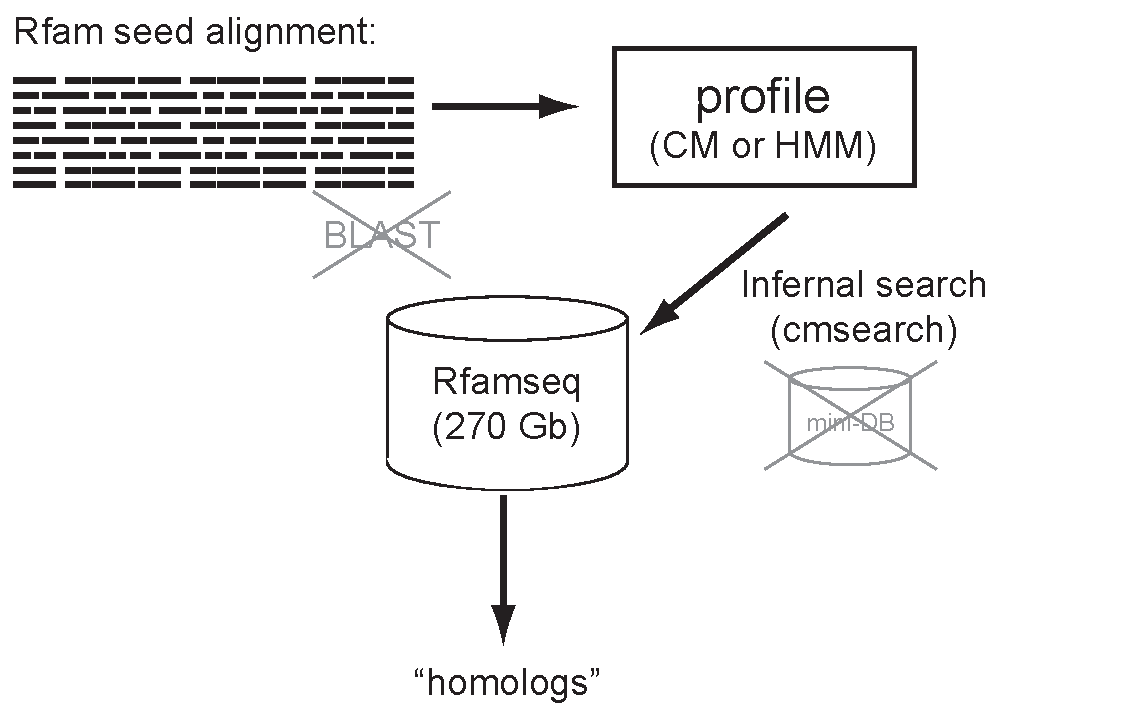
\includegraphics[width=8in]{figs/rfam-search-3}}

%\begin{center}
%\small
%Search results against Rfamseq for 200 random families:
%\begin{tabular}{l|rrr}
%strategy                   & time (h) & \# hits & \# unique hits \\ \hline
%Old (BLAST + Infernal 1.0) & 4069.8   &  179681 & 53 \\
%New (Infernal 1.1)         & 4222.2   &  201814 & 22312 \\
%\end{tabular}
%\end{center}

\vfill
\end{slide}
%%%%%%%%%%%%%%%%%%%%%%%%%%%%%%%%%%%%%%%%%%%%%%%%%%%%%%%%%%%%%%%%%%%%%%
\begin{slide}
\begin{center}

\textbf{Rfam 12.0 (2014)\footnote{Nawrocki, Burge et. al, NAR 43:D130-D137, 2015.}, 
first release without BLAST filtering}

\end{center}

\begin{center}
Search results against Rfamseq for 200 random families:

\medskip

\begin{tabular}{l|r|r|r}
strategy                   & time (h) & \# hits & \# unique hits \\ \hline
& & & \\
Old (BLAST + Infernal 1.0) & 4069.8   &  179,681 & 53 \\
& & & \\
New (Infernal 1.1)         & 4222.2   &  201,814 & 22,312 \\
\end{tabular}
\end{center}

\vfill
\end{slide}
%%%%%%%%%%%%%%%%%%%%%%%%%%%%%%%%%%%%%%%%%%%%%%%%%%%%%%%%%%%%%%%%%%%%%%
%\begin{slide}
%\begin{center}
%\small
%\end{center}
%
%\center{\includegraphics[width=10.5in]{figs/rfam-nar-table1-published}}
%
%\vfill
%\end{slide}
%%%%%%%%%%%%%%%%%%%%%%%%%%%%%%%%%%%%%%%%%%%%%%%%%%%%%%%%%%%%%%%%%%%%%%
\begin{slide}
\begin{center}
\textbf{Infernal 1.1 finds 11,000 new group I intron candidates}
\end{center}

%\center{\includegraphics[width=10.5in]{figs/rfam-nar-table1-published-gp1i-yellow}}
\center{\includegraphics[width=10.5in]{figs/rfam-nar-table1-published-gp1i-yellow-top5only}}

\vfill
\vfill
\small
\flushleft{Nawrocki, Burge et. al, NAR 43:D130-D137, 2015.} 
\end{slide}
%%%%%%%%%%%%%%%%%%%%%%%%%%%%%%%%%%%%%%%%%%%%%%%%%%%%%%%%%%%%%%%%%%%%%%%%%
\begin{slide}
\begin{center}
\textbf{It is now easier to use Rfam/Infernal to annotate your own
  datasets.} \\

\small
\begin{itemize}
\item A bacterial genome takes about 30 minutes for all 2474 models.
\end{itemize}

\end{center}

%\center{\includegraphics[width=10.5in]{figs/rfam-nar-table2-published}}
%\center{\includegraphics[width=10.5in]{figs/rfam-nar-table2-bac-yellow-yescaption}}
\center{\includegraphics[width=10.5in]{figs/rfam-nar-table2-bac-yellow-nocaption}}

\vfill
\small
\flushleft{Nawrocki, Burge et. al, NAR 43:D130-D137, 2015.} 
\end{slide}
%%%%%%%%%%%%%%%%%%%%%%%%%%%%%%%%%%%%%%%%%%%%%%%%%%%%%%%%%%%%%%%%%%%%%%%%%%
\begin{slide}
\begin{center}
\textbf{Outline of talk}

\begin{description}
\item[1.] Motivation: collecting homologs facilitates comparative
  sequence analysis.\\ 1965: Secondary structure determination of
  transfer RNA.
\item[2.] Sequence and sequence+structure profiles
%\item[3.] Benchmarking RNA homology search
\item[3.] Accelerating RNA homology search
\item[4.] Implications for Rfam
\item[\textcolor{red}{5.}] \textcolor{red}{New features in latest version of Infernal}
\end{description}

\end{center}
\vfill
\end{slide}
%%%%%%%%%%%%%%%%%%%%%%%%%%%%%%%%%%%%%%%%%%%%%%%%%%%%%%%%%%%%%%%%%%%%%%%%%%%
\begin{slide}
\begin{center}
\textbf{Infernal version 1.1.2 (July 2016)} \\
\end{center}

\medskip
\begin{itemize}
\item First release after moving to NCBI (without Infernal as my primary project)
\item Main difference is in the \texttt{cmscan} executable program 
\begin{itemize}
  \item faster
  \item annotates overlaps
\end{itemize}
\end{itemize}

%\begin{sreoutput}
%cmsearch:                                | cmscan:
%   for each query \textcolor{blue}{CM}                     |    for each query \textcolor{red}{sequence}
%       for each target \textcolor{red}{sequence}          |        for each target \textcolor{blue}{CM}
%           search for high-scoring hits  |            search for high-scoring hits
%                                         |
%                                         |
% hits reported per model                | - hits reported per sequence
%                                         | - reads as little model
%                                         |   info as possible
%\end{sreoutput}   

\vfill
\end{slide}
%%%%%%%%%%%%%%%%%%%%%%%%%%%%%%%%%%%%%%%%%%%%%%%%%%%%%%%%%%%%%%%%%%%%%%%%%%
\begin{slide}
\begin{center}
\textbf{cmsearch versus cmscan: a subtle but important difference}
\end{center}

\scriptsize
\begin{itemize}
\item cmsearch: hits reported by model
  \begin{itemize}
  \item \textcolor{red}{for each query} \textcolor{red}{CM}
    \begin{itemize}
    \item \textcolor{blue}{for each target} \textcolor{blue}{sequence}
      \begin{itemize}
      \item search for high-scoring hits
      \end{itemize}
    \end{itemize}
  \end{itemize}
\end{itemize}

\begin{itemize}
\item cmscan: hits reported by sequence
  \begin{itemize}
  \item \textcolor{blue}{for each query} \textcolor{blue}{sequence}
    \begin{itemize}
    \item \textcolor{red}{for each target} \textcolor{red}{CM}
      \begin{itemize}
      \item search for high-scoring hits
      \end{itemize}
    \end{itemize}
  \end{itemize}
\end{itemize}

\begin{itemize}
\item cmscan reads each CM for each sequence (all 2474 models)
\item if sequences are short this makes reading CMs a bottleneck
\end{itemize}

\vfill
\end{slide}
%%%%%%%%%%%%%%%%%%%%%%%%%%%%%%%%%%%%%%%%%%%%%%%%%%%%%%%%%%%%%%%%%%%%%%%%%%
\begin{slide}
\begin{center}
\textbf{cmsearch is faster than cmscan \\ for datasets with many short sequences}
\end{center}
\medskip

\small

Three sequence datasets:
\begin{enumerate}
  \item \emph{E. coli} genome: 4.6 Mb, 1 sequence
  \item ERS167139 (human gut microbiome, 454): 166 Mb (avg 423nt) 393K sequences 
%  \item ERS235581 (human gut microbiome, Illumina HiSeq): 53Mb (avg: 120nt), 440K sequences
  \item ERS235581 (human gut microbiome, HiSeq): 53Mb (avg: 120nt), 440K sequences
\end{enumerate}

\begin{center}
%Infernal v1.1.1 timings

\medskip
\medskip

%\tt
%\tiny
\begin{tabular}{l|r|r||r|r||r|r||}
         & \multicolumn{2}{c||}{E.coli}  & \multicolumn{2}{c||}{ERS167139} & \multicolumn{2}{c||}{ERS235581} \\
         & \multicolumn{2}{c||}{(4.6 mb, 1 seq)}  & \multicolumn{2}{c||}{(393K seqs, avg 423nt)} & \multicolumn{2}{c||}{(440K seqs, avg 120nt)} \\ \hline
program  & time & sec/seq & time & sec/seq & time & sec/seq \\ \hline
         &      &  & & & & \\
cmsearch v1.1.1  &     0.5h& 1746.7  & 28.2h   & 0.26    & 9.8h    & 0.08 \\
         &      &  & & & & \\
cmscan v1.1.1   &     0.5h& 1678.6  & 37.3h   & 0.34    & 20.5h   & 0.17 \\
         &      &  & & & & \\ 
\end{tabular}

\end{center}
\vfill
\end{slide}
%%%%%%%%%%%%%%%%%%%%%%%%%%%%%%%%%%%%%%%%%%%%%%%%%%%%%%%%%%%%%%%%%%%%%%%%%%
\begin{slide}
\begin{center}
\textbf{cmscan v1.1.2 stores CM model parameters \\ in memory instead of re-reading them for each sequence}
\end{center}
\medskip

\small

Three sequence datasets:
\begin{enumerate}
  \item \emph{E. coli} genome: 4.6 Mb, 1 sequence
  \item ERS167139 (human gut microbiome, 454): 166 Mb (avg 423nt) 393K sequences 
%  \item ERS235581 (human gut microbiome, Illumina HiSeq): 53Mb (avg: 120nt), 440K sequences
  \item ERS235581 (human gut microbiome, HiSeq): 53Mb (avg: 120nt), 440K sequences
\end{enumerate}

\begin{center}
%Infernal v1.1.1 timings

\medskip
\medskip

%\tt
%\tiny
\begin{tabular}{l|r|r||r|r||r|r||}
         & \multicolumn{2}{c||}{E.coli}  & \multicolumn{2}{c||}{ERS167139} & \multicolumn{2}{c||}{ERS235581} \\
         & \multicolumn{2}{c||}{(4.6 mb, 1 seq)}  & \multicolumn{2}{c||}{(393K seqs, avg 423nt)} & \multicolumn{2}{c||}{(440K seqs, avg 120nt)} \\ \hline
program  & time & sec/seq & time & sec/seq & time & sec/seq \\ \hline
         &      &  & & & & \\
cmsearch v1.1.1  &     0.5h& 1746.7  & 28.2h   & 0.26    & 9.8h    & 0.08 \\
         &      &  & & & & \\
cmscan v1.1.1   &     0.5h& 1678.6  & 37.3h   & 0.34    & 20.5h   & 0.17 \\
         &      &  & & & & \\ \hline
         &      &  & & & & \\ 
cmsearch v1.1.2  &     0.5h& 1808.2  & 25.3h   & 0.23    & 8.3h    & 0.07 \\
         &      &  & & & & \\
cmscan v1.1.2   &     0.5h& 1735.0  & \textcolor{blue}{26.7h}   & \textcolor{blue}{0.24}    & \textcolor{blue}{9.5h}   & \textcolor{blue}{0.08} \\
\end{tabular}

\end{center}
\vfill
\end{slide}
%%%%%%%%%%%%%%%%%%%%%%%%%%%%%%%%%%%%%%%%%%%%%%%%%%%%%%%%%%%%%%%%%%%%%%%%%%
\begin{slide}
\begin{center}
\textbf{Example of overlapping hits in cmscan v1.1.1 output} \\

\medskip
\medskip

\includegraphics[width=10in]{figs/overlap-examples-1p1p1}

\end{center}

\vfill
\end{slide}
%%%%%%%%%%%%%%%%%%%%%%%%%%%%%%%%%%%%%%%%%%%%%%%%%%%%%%%%%%%%%%%%%%%%%%%%%%
\begin{slide}
\begin{center}
\textbf{cmscan v1.1.2 marks up overlaps} \\

\medskip
\medskip

\includegraphics[width=10in]{figs/overlap-examples}

\end{center}

\vfill
\end{slide}
%%%%%%%%%%%%%%%%%%%%%%%%%%%%%%%%%%%%%%%%%%%%%%%%%%%%%%%%%%%%%%%%%%%%%%%%%%
\begin{comment}
\begin{slide}
\begin{center}
\textbf{cmscan v1.1.2 in ``hmmonly'' mode may be useful for \\ identifying RNAs in metagenomic datasets}

\end{center}

\vfill

\end{slide}
\end{comment}
%%%%%%%%%%%%%%%%%%%%%%%%%%%%%%%%%%%%%%%%%%%%%%%%%%%%%%%%%%%%%%%%%%%%%%%%%%
\begin{slide}

\large
\begin{center}
\large{\textbf{Acknowledgements}} \\

\vspace{0.5in}

\textbf{Alejandro Sch\"{a}ffer} \\
\textbf{David Landsman} \\
\textbf{David Lipman}

\vspace{0.5in}

\normalsize
%\begin{tabular}{llllll}
%Sean Eddy           & & & & & Michael Brent \\ 
%Elena Rivas         & & & & & Jeremy Buhler \\
%Tom Jones           & & & & & Justin Fay \\
%Diana Kolbe         & & & & & Jeff Gordon \\
%Seolkyoung Jung     & & & & & Rob Mitra \\
%Sergi Castellano    & & & & & Gary Stormo \\
%Fred Davis          & & & & & \\
%Lee Henry           & & & & & \\
%Michael Farrar      & & & & & \\
%Travis Wheeler      & & & & & \\
\begin{tabular}{l|l}
\textbf{Janelia} & \textbf{EBI (Rfam)} \\ \hline
Sean Eddy           & Alex Bateman \\
Elena Rivas         & Rob Finn \\
Travis Wheeler      & Anton Petrov \\
Tom Jones           & Ioanna Kalvari \\
Diana Kolbe         & Joanna Argasinska \\
Seolkyoung Jung     & Paul Gardner \\
Rob Finn            & Sarah Burge \\ 
Jody Clements       & Evan Floden \\
Fred Davis          & John Tate \\
Lee Henry           & Jen Daub \\
Michael Farrar      & \\
\end{tabular}

%\includegraphics[height=3in]{figs/jfrc-banner1}

\end{center}

\vfill
\end{slide}
%%%%%%%%%%%%%%%%%%%%%%%%%%%%%%%%%%%%%%%%%%%%%%%%%%%%%%%%%%%%%%%%%%%%%%
\begin{slide}
\begin{center}
\textbf{Applications of CMs}
\end{center}

\small
\begin{itemize}
\item homology search/alignment: Infernal,
  COVE, Rfam\footnote{E. P. Nawrocki,
    S. W. Burge et. al.
%    , A. Bateman, J. Daub, R. Y. Eberhardt, S. R. Eddy,
%    E. W. Floden, P. P. Gardner, T. A. Jones, J. Tate,
%    R. D. Finn. 
    NAR, 43:D130-D137, 2015.}, 
    Alternal\footnote{S. Janssen and R. Giegerich. BMC Bioinformatics
      2015, 16:178}, RNATOPS\footnote{Z. Huang et. al, 
      Bioinformatics, 24(20), 2281-2287, 2008.}
    
\item RNA discovery: CMfinder\footnote{Z. Yao, Z. Weinberg, W. L. Ruzzo,
  Bioinformatics 2006, 22(4), 445-452.}, 
  Zasha's pipeline(s)\footnote{Z. Weinberg, Z et. al. Nucleic acids
    research, 2007. 35(14), 4809-4819,
    Z. Weinberg et. al. Genome Biol, 2010. 11(3), R31.}
\item structure comparison: CMCompare\footnote{C. H. zu Siederdissen, and
  I. L. Hofacker Bioinformatics, 2010. 26(18), i453-i459.}
\item family-specific programs: 
\begin{itemize}
\item tRNAscan-SE\footnote{T. M. Lowe, S. R. Eddy. NAR,
    25:955-964, 1997.}, 
\item 16S/18S rRNA alignment: SSU-ALIGN\footnote{ E. P. Nawrocki. PhD
  Thesis: 2009, Washington University School of Medicine}
\item bacterial terminator identification: RNIE\footnote{P.P. Gardner
  et. al. Nucleic acids research, 2011, 39(14), 5845-5852.}
\end{itemize}
\end{itemize}

\vfill 
\end{slide}
\end{document}
